\documentclass[twoside]{book}

% Packages required by doxygen
\usepackage{fixltx2e}
\usepackage{calc}
\usepackage{doxygen}
\usepackage[export]{adjustbox} % also loads graphicx
\usepackage{graphicx}
\usepackage[utf8]{inputenc}
\usepackage{makeidx}
\usepackage{multicol}
\usepackage{multirow}
\PassOptionsToPackage{warn}{textcomp}
\usepackage{textcomp}
\usepackage[nointegrals]{wasysym}
\usepackage[table]{xcolor}

% Font selection
\usepackage[T1]{fontenc}
\usepackage[scaled=.90]{helvet}
\usepackage{courier}
\usepackage{amssymb}
\usepackage{sectsty}
\renewcommand{\familydefault}{\sfdefault}
\allsectionsfont{%
  \fontseries{bc}\selectfont%
  \color{darkgray}%
}
\renewcommand{\DoxyLabelFont}{%
  \fontseries{bc}\selectfont%
  \color{darkgray}%
}
\newcommand{\+}{\discretionary{\mbox{\scriptsize$\hookleftarrow$}}{}{}}

% Page & text layout
\usepackage{geometry}
\geometry{%
  a4paper,%
  top=2.5cm,%
  bottom=2.5cm,%
  left=2.5cm,%
  right=2.5cm%
}
\tolerance=750
\hfuzz=15pt
\hbadness=750
\setlength{\emergencystretch}{15pt}
\setlength{\parindent}{0cm}
\setlength{\parskip}{3ex plus 2ex minus 2ex}
\makeatletter
\renewcommand{\paragraph}{%
  \@startsection{paragraph}{4}{0ex}{-1.0ex}{1.0ex}{%
    \normalfont\normalsize\bfseries\SS@parafont%
  }%
}
\renewcommand{\subparagraph}{%
  \@startsection{subparagraph}{5}{0ex}{-1.0ex}{1.0ex}{%
    \normalfont\normalsize\bfseries\SS@subparafont%
  }%
}
\makeatother

% Headers & footers
\usepackage{fancyhdr}
\pagestyle{fancyplain}
\fancyhead[LE]{\fancyplain{}{\bfseries\thepage}}
\fancyhead[CE]{\fancyplain{}{}}
\fancyhead[RE]{\fancyplain{}{\bfseries\leftmark}}
\fancyhead[LO]{\fancyplain{}{\bfseries\rightmark}}
\fancyhead[CO]{\fancyplain{}{}}
\fancyhead[RO]{\fancyplain{}{\bfseries\thepage}}
\fancyfoot[LE]{\fancyplain{}{}}
\fancyfoot[CE]{\fancyplain{}{}}
\fancyfoot[RE]{\fancyplain{}{\bfseries\scriptsize Generated by Doxygen }}
\fancyfoot[LO]{\fancyplain{}{\bfseries\scriptsize Generated by Doxygen }}
\fancyfoot[CO]{\fancyplain{}{}}
\fancyfoot[RO]{\fancyplain{}{}}
\renewcommand{\footrulewidth}{0.4pt}
\renewcommand{\chaptermark}[1]{%
  \markboth{#1}{}%
}
\renewcommand{\sectionmark}[1]{%
  \markright{\thesection\ #1}%
}

% Indices & bibliography
\usepackage{natbib}
\usepackage[titles]{tocloft}
\setcounter{tocdepth}{3}
\setcounter{secnumdepth}{5}
\makeindex

% Hyperlinks (required, but should be loaded last)
\usepackage{ifpdf}
\ifpdf
  \usepackage[pdftex,pagebackref=true]{hyperref}
\else
  \usepackage[ps2pdf,pagebackref=true]{hyperref}
\fi
\hypersetup{%
  colorlinks=true,%
  linkcolor=blue,%
  citecolor=blue,%
  unicode%
}

% Custom commands
\newcommand{\clearemptydoublepage}{%
  \newpage{\pagestyle{empty}\cleardoublepage}%
}

\usepackage{caption}
\captionsetup{labelsep=space,justification=centering,font={bf},singlelinecheck=off,skip=4pt,position=top}

%===== C O N T E N T S =====

\begin{document}

% Titlepage & ToC
\hypersetup{pageanchor=false,
             bookmarksnumbered=true,
             pdfencoding=unicode
            }
\pagenumbering{alph}
\begin{titlepage}
\vspace*{7cm}
\begin{center}%
{\Large 2D Animation Software }\\
\vspace*{1cm}
{\large Generated by Doxygen 1.8.13}\\
\end{center}
\end{titlepage}
\clearemptydoublepage
\pagenumbering{roman}
\tableofcontents
\clearemptydoublepage
\pagenumbering{arabic}
\hypersetup{pageanchor=true}

%--- Begin generated contents ---
\chapter{Hierarchical Index}
\section{Class Hierarchy}
This inheritance list is sorted roughly, but not completely, alphabetically\+:\begin{DoxyCompactList}
\item \contentsline{section}{Adj\+Key\+Frame\+Data}{\pageref{struct_adj_key_frame_data}}{}
\item \contentsline{section}{Compare\+Frame}{\pageref{struct_compare_frame}}{}
\item \contentsline{section}{Compare\+Id}{\pageref{struct_compare_id}}{}
\item Drawable\begin{DoxyCompactList}
\item \contentsline{section}{Colour\+Panel}{\pageref{class_colour_panel}}{}
\item \contentsline{section}{I\+Tool}{\pageref{class_i_tool}}{}
\begin{DoxyCompactList}
\item \contentsline{section}{Colour\+Tool}{\pageref{class_colour_tool}}{}
\item \contentsline{section}{Joint\+Tool}{\pageref{class_joint_tool}}{}
\item \contentsline{section}{Shape\+Tool}{\pageref{class_shape_tool}}{}
\item \contentsline{section}{Transform\+Tool}{\pageref{class_transform_tool}}{}
\end{DoxyCompactList}
\item \contentsline{section}{Object}{\pageref{class_object}}{}
\item \contentsline{section}{Scroll\+Box}{\pageref{class_scroll_box}}{}
\item \contentsline{section}{Shapes}{\pageref{class_shapes}}{}
\item \contentsline{section}{Slider}{\pageref{class_slider}}{}
\item \contentsline{section}{Time\+Line}{\pageref{class_time_line}}{}
\item \contentsline{section}{Time\+Line\+Viewer}{\pageref{class_time_line_viewer}}{}
\item \contentsline{section}{Tool\+Box}{\pageref{class_tool_box}}{}
\end{DoxyCompactList}
\item \contentsline{section}{Event\+Handler}{\pageref{class_event_handler}}{}
\item \contentsline{section}{Frame\+Slot}{\pageref{struct_frame_slot}}{}
\item \contentsline{section}{Has\+Interaction\+Ptrs}{\pageref{class_has_interaction_ptrs}}{}
\begin{DoxyCompactList}
\item \contentsline{section}{I\+Tool}{\pageref{class_i_tool}}{}
\item \contentsline{section}{Tool\+Box}{\pageref{class_tool_box}}{}
\end{DoxyCompactList}
\item \contentsline{section}{Interaction\+Ptrs}{\pageref{struct_interaction_ptrs}}{}
\item \contentsline{section}{Interpolation\+Helper}{\pageref{class_interpolation_helper}}{}
\item \contentsline{section}{Key\+Frame}{\pageref{struct_key_frame}}{}
\item \contentsline{section}{Keyframe\+Manager}{\pageref{class_keyframe_manager}}{}
\item \contentsline{section}{Object\+Data}{\pageref{class_object_data}}{}
\item \contentsline{section}{Quad\+Part}{\pageref{class_quad_part}}{}
\begin{DoxyCompactList}
\item \contentsline{section}{Object}{\pageref{class_object}}{}
\end{DoxyCompactList}
\item Rectangle\+Shape\begin{DoxyCompactList}
\item \contentsline{section}{Button}{\pageref{class_button}}{}
\end{DoxyCompactList}
\item \contentsline{section}{S\+F\+M\+L\+Input\+Handler}{\pageref{class_s_f_m_l_input_handler}}{}
\item Shape\begin{DoxyCompactList}
\item \contentsline{section}{Ellipse\+Shape}{\pageref{class_ellipse_shape}}{}
\end{DoxyCompactList}
\item \contentsline{section}{Shape\+Key\+Frames}{\pageref{struct_shape_key_frames}}{}
\item \contentsline{section}{Shape\+Slot}{\pageref{struct_shape_slot}}{}
\item \contentsline{section}{Signal$<$ Args $>$}{\pageref{class_signal}}{}
\item \contentsline{section}{Signal$<$ bool $>$}{\pageref{class_signal}}{}
\item \contentsline{section}{Signal$<$ const flat\+\_\+set$<$ Shape\+Key\+Frames, Compare\+Id $>$ \&, Frame\+State $>$}{\pageref{class_signal}}{}
\item \contentsline{section}{Signal$<$ float $>$}{\pageref{class_signal}}{}
\item \contentsline{section}{Signal$<$ sf\+:\+:Mouse\+:\+:Button, bool $>$}{\pageref{class_signal}}{}
\item \contentsline{section}{Signal$<$ sf\+:\+:Vector2i $>$}{\pageref{class_signal}}{}
\item \contentsline{section}{Signal$<$ sf\+:\+:Vector2i, sf\+:\+:Vector2f $>$}{\pageref{class_signal}}{}
\item \contentsline{section}{Signal$<$ unsigned int $>$}{\pageref{class_signal}}{}
\item Sprite\begin{DoxyCompactList}
\item \contentsline{section}{Canvas}{\pageref{class_canvas}}{}
\end{DoxyCompactList}
\item \contentsline{section}{Q\+:\+:Time}{\pageref{class_q_1_1_time}}{}
\begin{DoxyCompactList}
\item \contentsline{section}{Q\+:\+:Timer}{\pageref{class_q_1_1_timer}}{}
\end{DoxyCompactList}
\item View\begin{DoxyCompactList}
\item \contentsline{section}{Camera}{\pageref{class_camera}}{}
\end{DoxyCompactList}
\end{DoxyCompactList}

\chapter{Class Index}
\section{Class List}
Here are the classes, structs, unions and interfaces with brief descriptions\+:\begin{DoxyCompactList}
\item\contentsline{section}{\hyperlink{struct_adj_key_frame_data}{Adj\+Key\+Frame\+Data} \\*Struct that holds adjacent keyframe data }{\pageref{struct_adj_key_frame_data}}{}
\item\contentsline{section}{\hyperlink{class_button}{Button} \\*A class that creates an easy to use button }{\pageref{class_button}}{}
\item\contentsline{section}{\hyperlink{class_camera}{Camera} \\*A class that inherits from sf\+::view that handles translations and zooming }{\pageref{class_camera}}{}
\item\contentsline{section}{\hyperlink{class_canvas}{Canvas} }{\pageref{class_canvas}}{}
\item\contentsline{section}{\hyperlink{class_colour_panel}{Colour\+Panel} \\*Provides a very simple UI for selecting a colour }{\pageref{class_colour_panel}}{}
\item\contentsline{section}{\hyperlink{class_colour_tool}{Colour\+Tool} \\*Used as a simple temporary means to recolour shapes }{\pageref{class_colour_tool}}{}
\item\contentsline{section}{\hyperlink{struct_compare_frame}{Compare\+Frame} \\*Comparator that orders frames via a the frame number }{\pageref{struct_compare_frame}}{}
\item\contentsline{section}{\hyperlink{struct_compare_id}{Compare\+Id} \\*Comparator that orders \hyperlink{struct_shape_key_frames}{Shape\+Key\+Frames} by their ID }{\pageref{struct_compare_id}}{}
\item\contentsline{section}{\hyperlink{class_ellipse_shape}{Ellipse\+Shape} \\*Custom S\+F\+ML shape class since sf\+::\+Circle cannont be scaled along the x and y axis individually }{\pageref{class_ellipse_shape}}{}
\item\contentsline{section}{\hyperlink{class_event_handler}{Event\+Handler} \\*Handles the connecting and registering of signals }{\pageref{class_event_handler}}{}
\item\contentsline{section}{\hyperlink{struct_frame_slot}{Frame\+Slot} \\*Struct that holds data for frame slots }{\pageref{struct_frame_slot}}{}
\item\contentsline{section}{\hyperlink{class_has_interaction_ptrs}{Has\+Interaction\+Ptrs} \\*Inherited by classes that need to used the interaction pointers }{\pageref{class_has_interaction_ptrs}}{}
\item\contentsline{section}{\hyperlink{struct_interaction_ptrs}{Interaction\+Ptrs} \\*Interaction pointers struct }{\pageref{struct_interaction_ptrs}}{}
\item\contentsline{section}{\hyperlink{class_interpolation_helper}{Interpolation\+Helper} \\*Contains methods for interplating between two positions }{\pageref{class_interpolation_helper}}{}
\item\contentsline{section}{\hyperlink{class_i_tool}{I\+Tool} \\*Handles generic methods that tools might need to use }{\pageref{class_i_tool}}{}
\item\contentsline{section}{\hyperlink{class_joint_tool}{Joint\+Tool} \\*Handles the linking joints between objest }{\pageref{class_joint_tool}}{}
\item\contentsline{section}{\hyperlink{struct_key_frame}{Key\+Frame} \\*Struct that holds frame number and its corresponding object data }{\pageref{struct_key_frame}}{}
\item\contentsline{section}{\hyperlink{class_keyframe_manager}{Keyframe\+Manager} \\*Manages keyframe data for objects Provides functionality to save, load, iterate and interpolate between keyframes }{\pageref{class_keyframe_manager}}{}
\item\contentsline{section}{\hyperlink{class_object}{Object} \\*Handles a quadpart and polyshape to make up a more transformable object that just using an S\+F\+ML shape }{\pageref{class_object}}{}
\item\contentsline{section}{\hyperlink{class_object_data}{Object\+Data} \\*Struct that holds object data i.\+e. position, rotation and vertices }{\pageref{class_object_data}}{}
\item\contentsline{section}{\hyperlink{class_quad_part}{Quad\+Part} \\*A class that can handle more complex transformations and store joint data Made from a basic vertex array to allow for more precise transformations than that of an S\+F\+ML shape }{\pageref{class_quad_part}}{}
\item\contentsline{section}{\hyperlink{class_scroll_box}{Scroll\+Box} }{\pageref{class_scroll_box}}{}
\item\contentsline{section}{\hyperlink{class_s_f_m_l_input_handler}{S\+F\+M\+L\+Input\+Handler} \\*Class that manages S\+F\+ML\textquotesingle{}s input events and notifies thier corresponding signals }{\pageref{class_s_f_m_l_input_handler}}{}
\item\contentsline{section}{\hyperlink{struct_shape_key_frames}{Shape\+Key\+Frames} \\*Struct that holds the ID and corresponding keyframes }{\pageref{struct_shape_key_frames}}{}
\item\contentsline{section}{\hyperlink{class_shapes}{Shapes} \\*Container class that handles the creation and getting of objects via I\+Ds }{\pageref{class_shapes}}{}
\item\contentsline{section}{\hyperlink{struct_shape_slot}{Shape\+Slot} \\*Struct that holds data for shape slots and their corrisponding frame slots }{\pageref{struct_shape_slot}}{}
\item\contentsline{section}{\hyperlink{class_shape_tool}{Shape\+Tool} \\*Handles the drawing and creation of a shape }{\pageref{class_shape_tool}}{}
\item\contentsline{section}{\hyperlink{class_signal}{Signal$<$ Args $>$} \\*Handles the connections of call back functions }{\pageref{class_signal}}{}
\item\contentsline{section}{\hyperlink{class_slider}{Slider} \\*Used to create a very simple slider }{\pageref{class_slider}}{}
\item\contentsline{section}{\hyperlink{class_q_1_1_time}{Q\+::\+Time} }{\pageref{class_q_1_1_time}}{}
\item\contentsline{section}{\hyperlink{class_time_line}{Time\+Line} \\*Creates and manages a user interface to deal with \char`\"{}\+Shape\+Key\+Frame\char`\"{} data }{\pageref{class_time_line}}{}
\item\contentsline{section}{\hyperlink{class_time_line_viewer}{Time\+Line\+Viewer} }{\pageref{class_time_line_viewer}}{}
\item\contentsline{section}{\hyperlink{class_q_1_1_timer}{Q\+::\+Timer} }{\pageref{class_q_1_1_timer}}{}
\item\contentsline{section}{\hyperlink{class_tool_box}{Tool\+Box} \\*Handles the creation and switching of tools }{\pageref{class_tool_box}}{}
\item\contentsline{section}{\hyperlink{class_transform_tool}{Transform\+Tool} \\*Handles the interaction of transforming an object }{\pageref{class_transform_tool}}{}
\end{DoxyCompactList}

\chapter{Class Documentation}
\hypertarget{struct_adj_key_frame_data}{}\section{Adj\+Key\+Frame\+Data Struct Reference}
\label{struct_adj_key_frame_data}\index{Adj\+Key\+Frame\+Data@{Adj\+Key\+Frame\+Data}}


Struct that holds adjacent keyframe data.  




{\ttfamily \#include $<$Anim\+Structs.\+h$>$}

\subsection*{Public Attributes}
\begin{DoxyCompactItemize}
\item 
\mbox{\Hypertarget{struct_adj_key_frame_data_adcc624fb8fe7e1efa2b03b69b62cbb11}\label{struct_adj_key_frame_data_adcc624fb8fe7e1efa2b03b69b62cbb11}} 
int {\bfseries Next}
\item 
\mbox{\Hypertarget{struct_adj_key_frame_data_aacb8e25c9c2db5e6dc1d58656acc8839}\label{struct_adj_key_frame_data_aacb8e25c9c2db5e6dc1d58656acc8839}} 
int {\bfseries Prev}
\item 
\mbox{\Hypertarget{struct_adj_key_frame_data_a8353a575cc655e06f4dc2af38be629d2}\label{struct_adj_key_frame_data_a8353a575cc655e06f4dc2af38be629d2}} 
bool {\bfseries Visible}
\end{DoxyCompactItemize}


\subsection{Detailed Description}
Struct that holds adjacent keyframe data. 

The documentation for this struct was generated from the following file\+:\begin{DoxyCompactItemize}
\item 
D\+:/\+Sam/\+D\+M\+U/\+Year 3/\+I\+M\+A\+T3451 -\/ Final/\+Animation project repo/\+Animation Tool/\+Animation Project/include/Anim\+Structs.\+h\end{DoxyCompactItemize}

\hypertarget{class_button}{}\section{Button Class Reference}
\label{class_button}\index{Button@{Button}}


A class that creates an easy to use button.  




{\ttfamily \#include $<$Button.\+h$>$}

Inheritance diagram for Button\+:\begin{figure}[H]
\begin{center}
\leavevmode
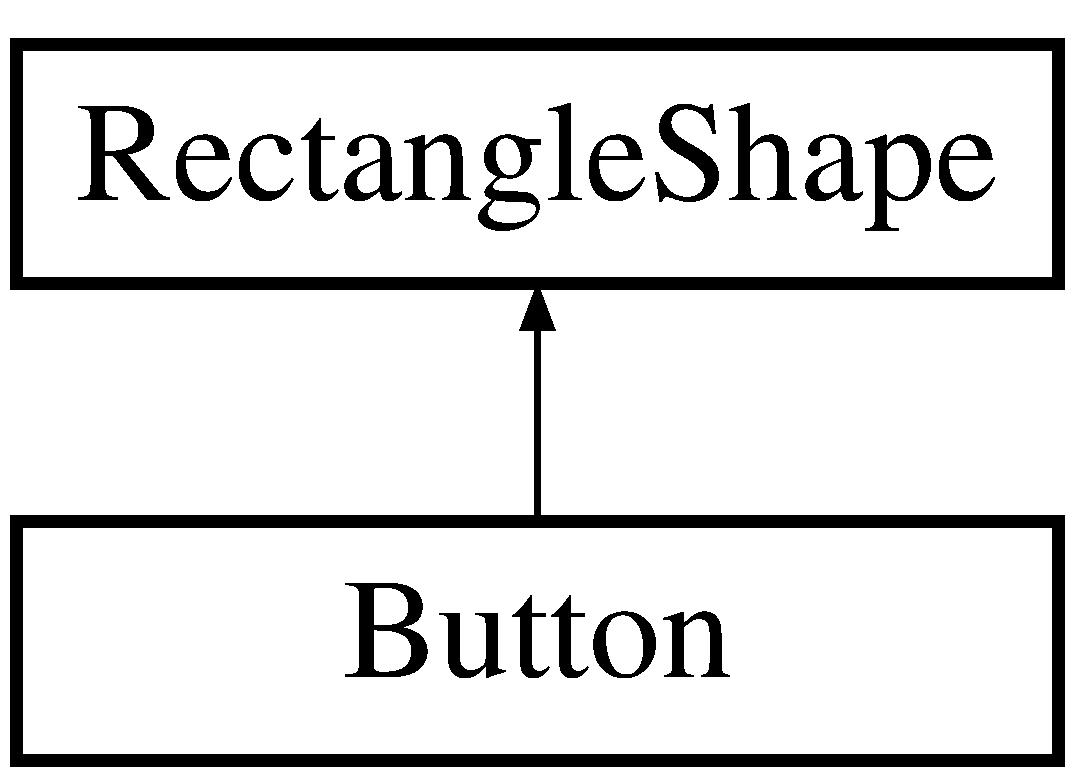
\includegraphics[height=2.000000cm]{class_button}
\end{center}
\end{figure}
\subsection*{Public Member Functions}
\begin{DoxyCompactItemize}
\item 
\mbox{\Hypertarget{class_button_ab1efa067f59ac17af501ba523527cee6}\label{class_button_ab1efa067f59ac17af501ba523527cee6}} 
\hyperlink{class_button_ab1efa067f59ac17af501ba523527cee6}{Button} (std\+::string p\+\_\+\+Signal\+Name, std\+::string p\+\_\+\+Icon\+File\+Path, const sf\+::\+Vector2f \&p\+\_\+\+Pos, const sf\+::\+Vector2f \&p\+\_\+\+Size)
\begin{DoxyCompactList}\small\item\em Constructor. \end{DoxyCompactList}\item 
\mbox{\Hypertarget{class_button_acf51cb6628e0a1fd57d07201634ca859}\label{class_button_acf51cb6628e0a1fd57d07201634ca859}} 
void \hyperlink{class_button_acf51cb6628e0a1fd57d07201634ca859}{On\+Mouse\+Click} (bool p\+\_\+\+State)
\begin{DoxyCompactList}\small\item\em Callback for mouse click events. \end{DoxyCompactList}\item 
\mbox{\Hypertarget{class_button_a542274c2ff280252d8694e62d269da40}\label{class_button_a542274c2ff280252d8694e62d269da40}} 
void \hyperlink{class_button_a542274c2ff280252d8694e62d269da40}{On\+Mouse\+Move} (sf\+::\+Vector2i p\+\_\+\+Pos)
\begin{DoxyCompactList}\small\item\em Callback for mouse move events. \end{DoxyCompactList}\end{DoxyCompactItemize}
\subsection*{Public Attributes}
\begin{DoxyCompactItemize}
\item 
\mbox{\Hypertarget{class_button_afb6f1c9a85ffe02859e54b71c2bb372b}\label{class_button_afb6f1c9a85ffe02859e54b71c2bb372b}} 
\hyperlink{class_signal}{Signal} \hyperlink{class_button_afb6f1c9a85ffe02859e54b71c2bb372b}{on\+Clicked}
\begin{DoxyCompactList}\small\item\em \hyperlink{class_signal}{Signal} that the button has been clicked. \end{DoxyCompactList}\item 
\mbox{\Hypertarget{class_button_a9ba6e57a49de78557823cc4a775e7030}\label{class_button_a9ba6e57a49de78557823cc4a775e7030}} 
\hyperlink{class_signal}{Signal}$<$ bool $>$ \hyperlink{class_button_a9ba6e57a49de78557823cc4a775e7030}{on\+Any\+Button\+Over}
\begin{DoxyCompactList}\small\item\em Redundant signal. \end{DoxyCompactList}\end{DoxyCompactItemize}


\subsection{Detailed Description}
A class that creates an easy to use button. 

The documentation for this class was generated from the following file\+:\begin{DoxyCompactItemize}
\item 
D\+:/\+Sam/\+D\+M\+U/\+Year 3/\+I\+M\+A\+T3451 -\/ Final/\+Animation project repo/\+Animation Tool/\+Animation Project/include/Button.\+h\end{DoxyCompactItemize}

\hypertarget{class_camera}{}\section{Camera Class Reference}
\label{class_camera}\index{Camera@{Camera}}


A class that inherits from sf\+::view that handles translations and zooming.  




{\ttfamily \#include $<$Camera.\+h$>$}

Inheritance diagram for Camera\+:\begin{figure}[H]
\begin{center}
\leavevmode
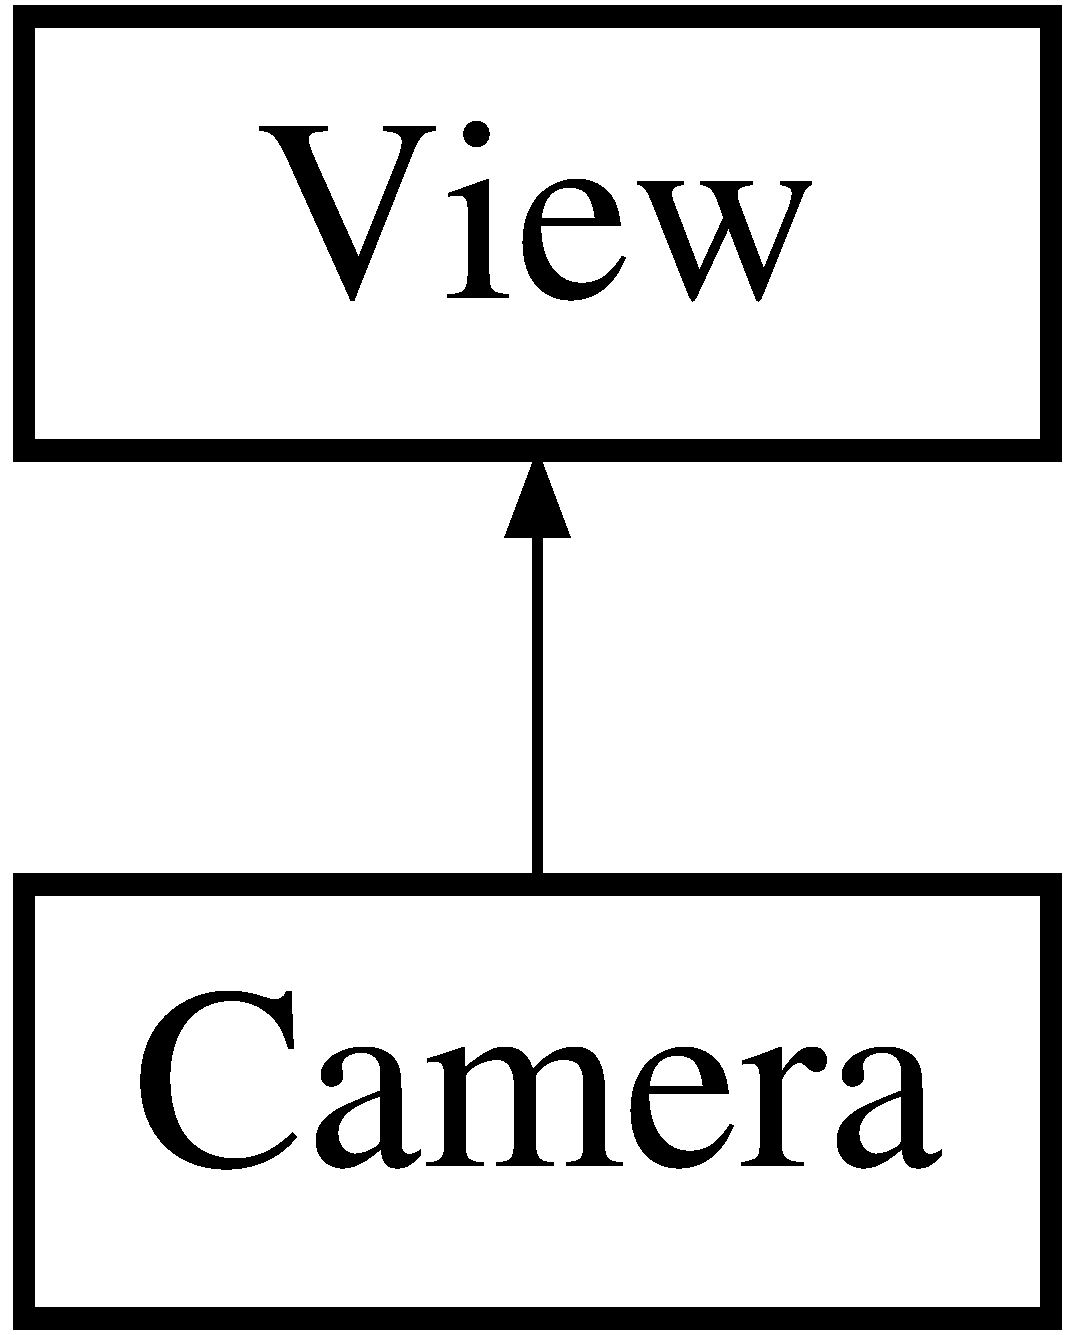
\includegraphics[height=2.000000cm]{class_camera}
\end{center}
\end{figure}
\subsection*{Public Member Functions}
\begin{DoxyCompactItemize}
\item 
\mbox{\Hypertarget{class_camera_a0c1efce0a93d56215af15a6bc88f360f}\label{class_camera_a0c1efce0a93d56215af15a6bc88f360f}} 
\hyperlink{class_camera_a0c1efce0a93d56215af15a6bc88f360f}{Camera} (sf\+::\+Vector2f p\+\_\+\+Center, sf\+::\+Vector2f p\+\_\+\+Size)
\begin{DoxyCompactList}\small\item\em constructor that takes a centre position and a size \end{DoxyCompactList}\item 
\mbox{\Hypertarget{class_camera_a58eedba9725c44625b3e983221aaf444}\label{class_camera_a58eedba9725c44625b3e983221aaf444}} 
void \hyperlink{class_camera_a58eedba9725c44625b3e983221aaf444}{On\+Mouse\+Click} (sf\+::\+Mouse\+::\+Button p\+\_\+\+Button, bool p\+\_\+b\+State)
\begin{DoxyCompactList}\small\item\em Callback for mouse click events. \end{DoxyCompactList}\item 
\mbox{\Hypertarget{class_camera_a43f67138a331c8fe5d5fc144b47c0a41}\label{class_camera_a43f67138a331c8fe5d5fc144b47c0a41}} 
void \hyperlink{class_camera_a43f67138a331c8fe5d5fc144b47c0a41}{On\+Mouse\+Wheel} (float p\+\_\+f\+Delta)
\begin{DoxyCompactList}\small\item\em Callback for mouse wheel events. \end{DoxyCompactList}\item 
\mbox{\Hypertarget{class_camera_adf59388a392cf0195b3b1076d9fd27dd}\label{class_camera_adf59388a392cf0195b3b1076d9fd27dd}} 
void \hyperlink{class_camera_adf59388a392cf0195b3b1076d9fd27dd}{On\+Mouse\+Move} (sf\+::\+Vector2i p\+\_\+\+Position)
\begin{DoxyCompactList}\small\item\em Callback for mouse move events. \end{DoxyCompactList}\item 
\mbox{\Hypertarget{class_camera_ab6170a0b0ed8ef476d658fc18cf1c96b}\label{class_camera_ab6170a0b0ed8ef476d658fc18cf1c96b}} 
sf\+::\+Vector2f \hyperlink{class_camera_ab6170a0b0ed8ef476d658fc18cf1c96b}{get\+Scale} ()
\begin{DoxyCompactList}\small\item\em Scale getter. \end{DoxyCompactList}\end{DoxyCompactItemize}


\subsection{Detailed Description}
A class that inherits from sf\+::view that handles translations and zooming. 

The documentation for this class was generated from the following file\+:\begin{DoxyCompactItemize}
\item 
D\+:/\+Sam/\+D\+M\+U/\+Year 3/\+I\+M\+A\+T3451 -\/ Final/\+Animation project repo/\+Animation Tool/\+Animation Project/include/Camera.\+h\end{DoxyCompactItemize}

\hypertarget{class_canvas}{}\section{Canvas Class Reference}
\label{class_canvas}\index{Canvas@{Canvas}}
Inheritance diagram for Canvas\+:\begin{figure}[H]
\begin{center}
\leavevmode
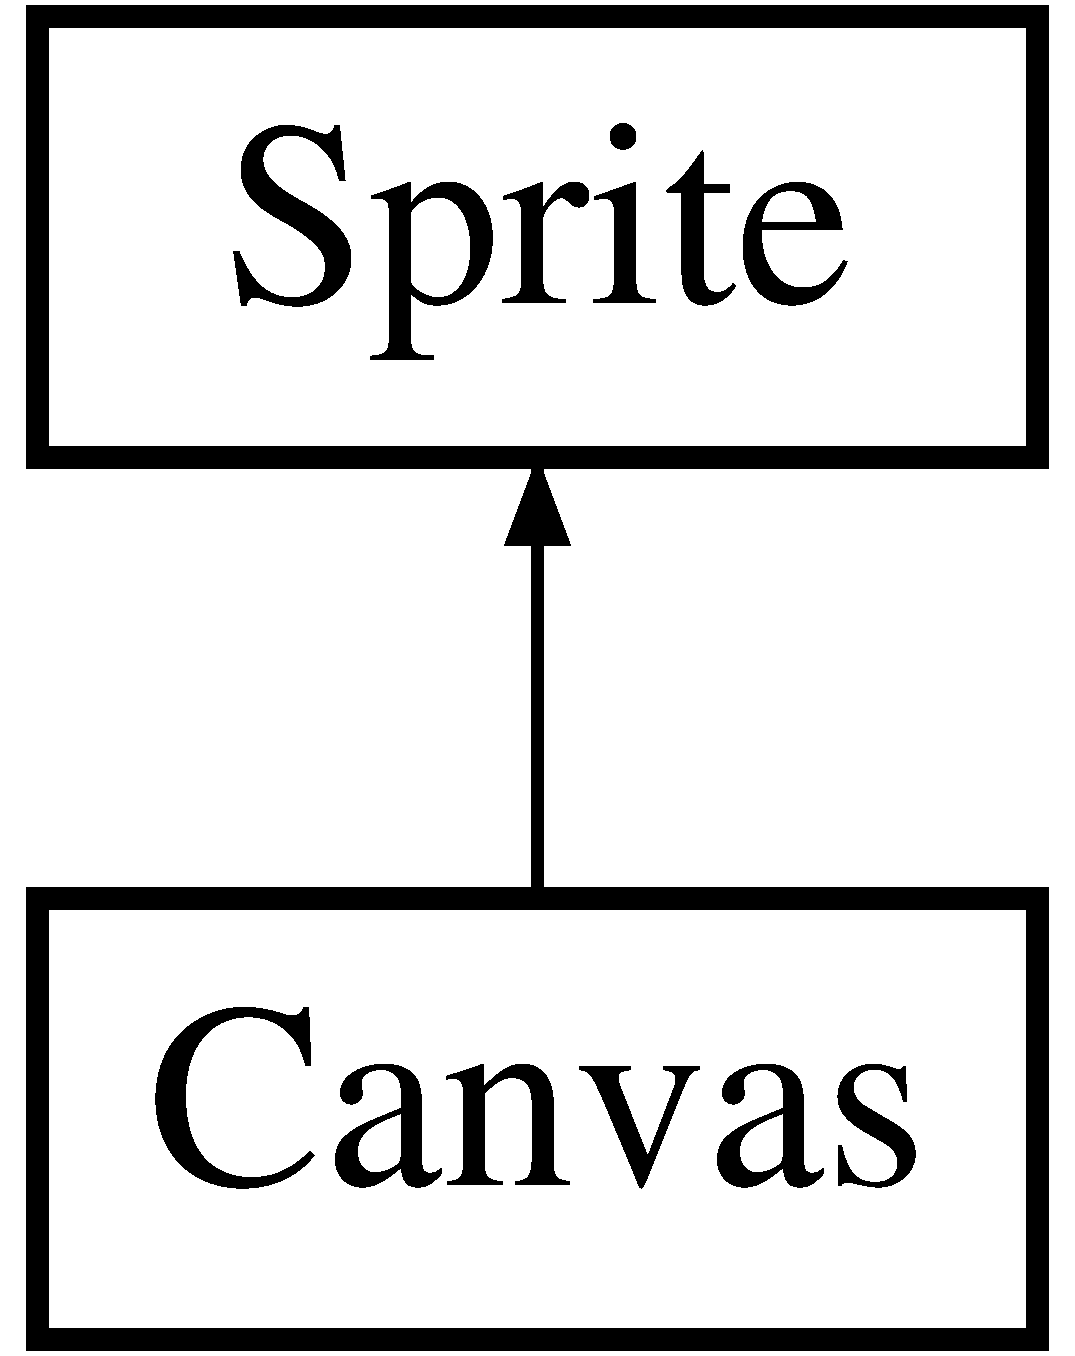
\includegraphics[height=2.000000cm]{class_canvas}
\end{center}
\end{figure}
\subsection*{Public Member Functions}
\begin{DoxyCompactItemize}
\item 
\mbox{\Hypertarget{class_canvas_a986afb603e6a8182bef8c45f06494221}\label{class_canvas_a986afb603e6a8182bef8c45f06494221}} 
{\bfseries Canvas} (sf\+::\+Render\+Window $\ast$p\+\_\+p\+Window)
\item 
\mbox{\Hypertarget{class_canvas_a201413f418eef9b0336772401ec009ee}\label{class_canvas_a201413f418eef9b0336772401ec009ee}} 
void {\bfseries Update} ()
\item 
\mbox{\Hypertarget{class_canvas_a19cd4eba59f4e18830d9ac1be53210ff}\label{class_canvas_a19cd4eba59f4e18830d9ac1be53210ff}} 
void {\bfseries Draw} (const sf\+::\+Drawable \&p\+\_\+\+Drawable)
\item 
\mbox{\Hypertarget{class_canvas_a6fa937d64a95ad0b4510c3227e3bed3d}\label{class_canvas_a6fa937d64a95ad0b4510c3227e3bed3d}} 
void {\bfseries Clear} (const sf\+::\+Color \&color)
\item 
\mbox{\Hypertarget{class_canvas_afc0c7c0669202f0c41fa17ecd81abb1f}\label{class_canvas_afc0c7c0669202f0c41fa17ecd81abb1f}} 
void {\bfseries Display} ()
\item 
\mbox{\Hypertarget{class_canvas_a2c0019f93d948b0b0cd69d01862192b8}\label{class_canvas_a2c0019f93d948b0b0cd69d01862192b8}} 
void {\bfseries Handle\+Mouse\+Input} (sf\+::\+Mouse\+::\+Button p\+\_\+\+Button, bool p\+\_\+b\+State)
\item 
\mbox{\Hypertarget{class_canvas_ab5e67ca2616e2ac672082a0628dc1c36}\label{class_canvas_ab5e67ca2616e2ac672082a0628dc1c36}} 
sf\+::\+Render\+Texture $\ast$ {\bfseries Rend\+Tex\+Ptr} ()
\end{DoxyCompactItemize}


The documentation for this class was generated from the following files\+:\begin{DoxyCompactItemize}
\item 
D\+:/\+Sam/\+D\+M\+U/\+Year 3/\+I\+M\+A\+T3451 -\/ Final/\+Animation project repo/\+Animation Tool/\+Animation Project/include/Canvas.\+h\item 
D\+:/\+Sam/\+D\+M\+U/\+Year 3/\+I\+M\+A\+T3451 -\/ Final/\+Animation project repo/\+Animation Tool/\+Animation Project/include/Canvas.\+cpp\end{DoxyCompactItemize}

\hypertarget{class_colour_panel}{}\section{Colour\+Panel Class Reference}
\label{class_colour_panel}\index{Colour\+Panel@{Colour\+Panel}}


Provides a very simple UI for selecting a colour.  




{\ttfamily \#include $<$Colour\+Panel.\+h$>$}

Inheritance diagram for Colour\+Panel\+:\begin{figure}[H]
\begin{center}
\leavevmode
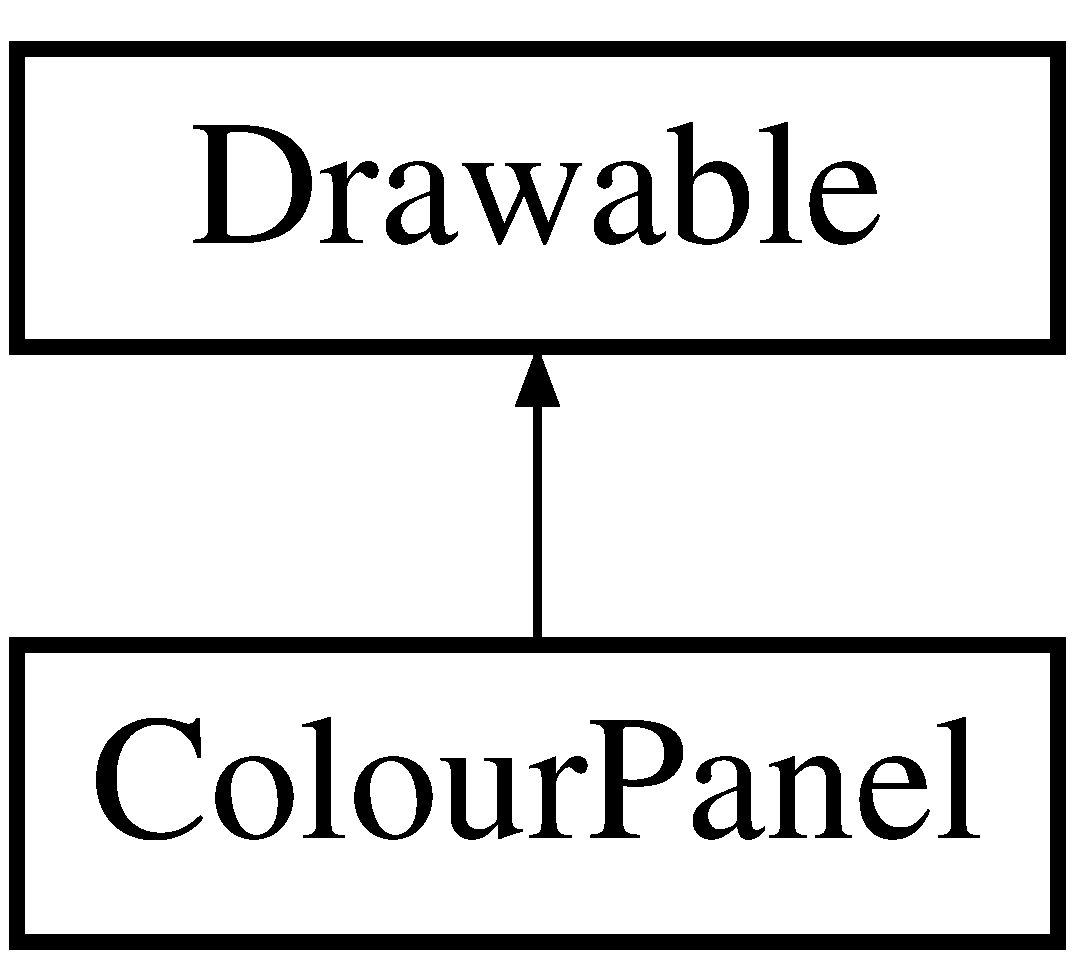
\includegraphics[height=2.000000cm]{class_colour_panel}
\end{center}
\end{figure}
\subsection*{Public Member Functions}
\begin{DoxyCompactItemize}
\item 
\mbox{\Hypertarget{class_colour_panel_a5dc33d83d0aafa0c936c3989e6f11e39}\label{class_colour_panel_a5dc33d83d0aafa0c936c3989e6f11e39}} 
\hyperlink{class_colour_panel_a5dc33d83d0aafa0c936c3989e6f11e39}{Colour\+Panel} (sf\+::\+Vector2f p\+\_\+\+Pos)
\begin{DoxyCompactList}\small\item\em Constructor that takes the position for the panel. \end{DoxyCompactList}\item 
\mbox{\Hypertarget{class_colour_panel_ad7a1677b7e21b6d1c3667358040f4719}\label{class_colour_panel_ad7a1677b7e21b6d1c3667358040f4719}} 
sf\+::\+Color \hyperlink{class_colour_panel_ad7a1677b7e21b6d1c3667358040f4719}{get\+Colour} ()
\begin{DoxyCompactList}\small\item\em Colour getter. \end{DoxyCompactList}\item 
\mbox{\Hypertarget{class_colour_panel_ac9299d66643be6579c3541724c88d2de}\label{class_colour_panel_ac9299d66643be6579c3541724c88d2de}} 
void \hyperlink{class_colour_panel_ac9299d66643be6579c3541724c88d2de}{Update} (float p\+\_\+\+Delta\+Time)
\begin{DoxyCompactList}\small\item\em Update method. \end{DoxyCompactList}\item 
\mbox{\Hypertarget{class_colour_panel_a6f76355771589d3c8240d69777f76530}\label{class_colour_panel_a6f76355771589d3c8240d69777f76530}} 
void \hyperlink{class_colour_panel_a6f76355771589d3c8240d69777f76530}{Handle\+Mouse\+Input} (sf\+::\+Mouse\+::\+Button p\+\_\+\+Button, bool p\+\_\+b\+State)
\begin{DoxyCompactList}\small\item\em Callback for handling mouse button events. \end{DoxyCompactList}\item 
\mbox{\Hypertarget{class_colour_panel_af8a216658cd97964e268626ef469dc15}\label{class_colour_panel_af8a216658cd97964e268626ef469dc15}} 
void \hyperlink{class_colour_panel_af8a216658cd97964e268626ef469dc15}{Handle\+Mouse\+Move} (sf\+::\+Vector2i p\+\_\+\+Position)
\begin{DoxyCompactList}\small\item\em Callback for handling mouse move events. \end{DoxyCompactList}\item 
\mbox{\Hypertarget{class_colour_panel_a9a763ee1e08cee05d93e95a7c0e87ca5}\label{class_colour_panel_a9a763ee1e08cee05d93e95a7c0e87ca5}} 
void \hyperlink{class_colour_panel_a9a763ee1e08cee05d93e95a7c0e87ca5}{draw} (sf\+::\+Render\+Target \&target, sf\+::\+Render\+States states) const
\begin{DoxyCompactList}\small\item\em Draw method for drawing the panel. \end{DoxyCompactList}\end{DoxyCompactItemize}


\subsection{Detailed Description}
Provides a very simple UI for selecting a colour. 

The documentation for this class was generated from the following file\+:\begin{DoxyCompactItemize}
\item 
D\+:/\+Sam/\+D\+M\+U/\+Year 3/\+I\+M\+A\+T3451 -\/ Final/\+Animation project repo/\+Animation Tool/\+Animation Project/include/Colour\+Panel.\+h\end{DoxyCompactItemize}

\hypertarget{class_colour_tool}{}\section{Colour\+Tool Class Reference}
\label{class_colour_tool}\index{Colour\+Tool@{Colour\+Tool}}


Used as a simple temporary means to recolour shapes.  




{\ttfamily \#include $<$Colour\+Tool.\+h$>$}

Inheritance diagram for Colour\+Tool\+:\begin{figure}[H]
\begin{center}
\leavevmode
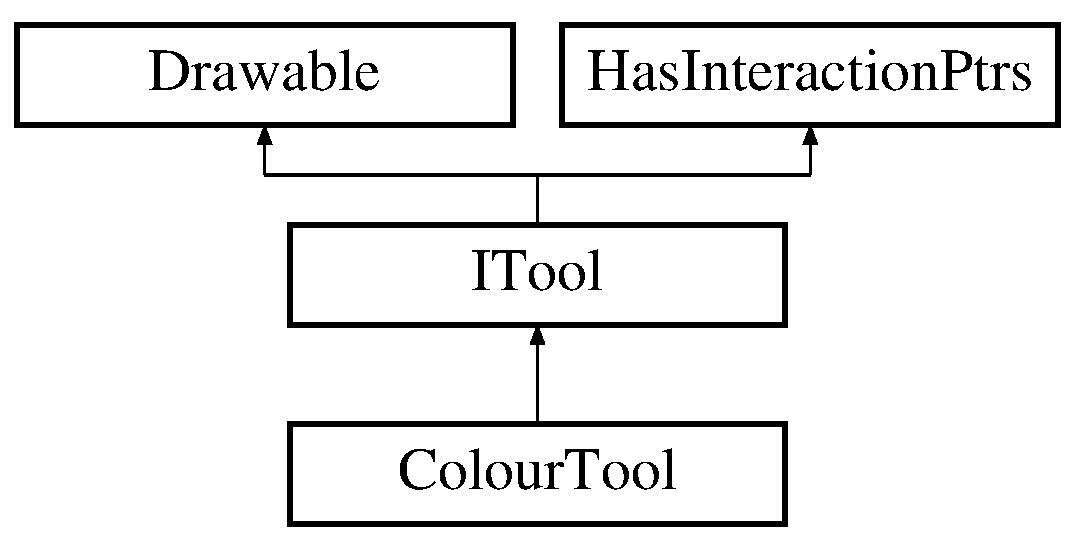
\includegraphics[height=3.000000cm]{class_colour_tool}
\end{center}
\end{figure}
\subsection*{Public Member Functions}
\begin{DoxyCompactItemize}
\item 
\mbox{\Hypertarget{class_colour_tool_aaedac79d91816998884ea165f1b58da0}\label{class_colour_tool_aaedac79d91816998884ea165f1b58da0}} 
\hyperlink{class_colour_tool_aaedac79d91816998884ea165f1b58da0}{Colour\+Tool} (\hyperlink{struct_interaction_ptrs}{Interaction\+Ptrs} $\ast$p\+\_\+p\+SP)
\begin{DoxyCompactList}\small\item\em constructor that takes interaction\+Ptrs that contains useful classes needed to recolour shapes \end{DoxyCompactList}\item 
\mbox{\Hypertarget{class_colour_tool_a8f6f08e54a1e074740aee812bbe54db0}\label{class_colour_tool_a8f6f08e54a1e074740aee812bbe54db0}} 
void \hyperlink{class_colour_tool_a8f6f08e54a1e074740aee812bbe54db0}{Update} (float p\+\_\+\+Delta\+Time) override
\begin{DoxyCompactList}\small\item\em Update method. \end{DoxyCompactList}\item 
\mbox{\Hypertarget{class_colour_tool_a2a499beddabdf11b1d982c68174df8ad}\label{class_colour_tool_a2a499beddabdf11b1d982c68174df8ad}} 
void \hyperlink{class_colour_tool_a2a499beddabdf11b1d982c68174df8ad}{On\+Mouse\+Click} (sf\+::\+Mouse\+::\+Button p\+\_\+\+Button, bool p\+\_\+b\+State) override
\begin{DoxyCompactList}\small\item\em Callback method that is notified on a mouse button event. \end{DoxyCompactList}\item 
\mbox{\Hypertarget{class_colour_tool_a02ad228f089cf99ba9f56b66f18de24b}\label{class_colour_tool_a02ad228f089cf99ba9f56b66f18de24b}} 
void \hyperlink{class_colour_tool_a02ad228f089cf99ba9f56b66f18de24b}{On\+Mouse\+Move} (sf\+::\+Vector2i p\+\_\+\+Mouse\+Window\+Pos, sf\+::\+Vector2f p\+\_\+\+Mouse\+World\+Pos) override
\begin{DoxyCompactList}\small\item\em Callback method that is notified on a mouse move extra event. \end{DoxyCompactList}\item 
\mbox{\Hypertarget{class_colour_tool_a60f7a883b45ab06a0461988fa48e38d5}\label{class_colour_tool_a60f7a883b45ab06a0461988fa48e38d5}} 
void \hyperlink{class_colour_tool_a60f7a883b45ab06a0461988fa48e38d5}{draw} (sf\+::\+Render\+Target \&target, sf\+::\+Render\+States states) const
\begin{DoxyCompactList}\small\item\em draw method that draws the colour panel \end{DoxyCompactList}\end{DoxyCompactItemize}
\subsection*{Additional Inherited Members}


\subsection{Detailed Description}
Used as a simple temporary means to recolour shapes. 

The documentation for this class was generated from the following file\+:\begin{DoxyCompactItemize}
\item 
D\+:/\+Sam/\+D\+M\+U/\+Year 3/\+I\+M\+A\+T3451 -\/ Final/\+Animation project repo/\+Animation Tool/\+Animation Project/include/Colour\+Tool.\+h\end{DoxyCompactItemize}

\hypertarget{struct_compare_frame}{}\section{Compare\+Frame Struct Reference}
\label{struct_compare_frame}\index{Compare\+Frame@{Compare\+Frame}}


Comparator that orders frames via a the frame number.  




{\ttfamily \#include $<$Anim\+Structs.\+h$>$}

\subsection*{Public Types}
\begin{DoxyCompactItemize}
\item 
\mbox{\Hypertarget{struct_compare_frame_a9ee39ccc90c3a72c8f91e338e594f5b8}\label{struct_compare_frame_a9ee39ccc90c3a72c8f91e338e594f5b8}} 
using {\bfseries is\+\_\+transparent} = void
\end{DoxyCompactItemize}
\subsection*{Public Member Functions}
\begin{DoxyCompactItemize}
\item 
\mbox{\Hypertarget{struct_compare_frame_a4a1d27b71a2080650af0f20dac2b8d68}\label{struct_compare_frame_a4a1d27b71a2080650af0f20dac2b8d68}} 
bool {\bfseries operator()} (const \hyperlink{struct_key_frame}{Key\+Frame} \&p\+\_\+A, const \hyperlink{struct_key_frame}{Key\+Frame} \&p\+\_\+B) const
\item 
\mbox{\Hypertarget{struct_compare_frame_aad891f00abf4c72b158028b5728f259d}\label{struct_compare_frame_aad891f00abf4c72b158028b5728f259d}} 
bool {\bfseries operator()} (unsigned int p\+\_\+\+Frame, const \hyperlink{struct_key_frame}{Key\+Frame} \&p\+\_\+\+Shape\+Key\+Frames) const
\item 
\mbox{\Hypertarget{struct_compare_frame_ae8814c26673640406f5989e92afc6a33}\label{struct_compare_frame_ae8814c26673640406f5989e92afc6a33}} 
bool {\bfseries operator()} (const \hyperlink{struct_key_frame}{Key\+Frame} \&p\+\_\+\+Shape\+Key\+Frames, unsigned int p\+\_\+\+Frame) const
\end{DoxyCompactItemize}


\subsection{Detailed Description}
Comparator that orders frames via a the frame number. 

The documentation for this struct was generated from the following file\+:\begin{DoxyCompactItemize}
\item 
D\+:/\+Sam/\+D\+M\+U/\+Year 3/\+I\+M\+A\+T3451 -\/ Final/\+Animation project repo/\+Animation Tool/\+Animation Project/include/Anim\+Structs.\+h\end{DoxyCompactItemize}

\hypertarget{struct_compare_id}{}\section{Compare\+Id Struct Reference}
\label{struct_compare_id}\index{Compare\+Id@{Compare\+Id}}


Comparator that orders \hyperlink{struct_shape_key_frames}{Shape\+Key\+Frames} by their ID.  




{\ttfamily \#include $<$Anim\+Structs.\+h$>$}

\subsection*{Public Types}
\begin{DoxyCompactItemize}
\item 
\mbox{\Hypertarget{struct_compare_id_a7dd0fa1db14a369c56c98ec8339ecf07}\label{struct_compare_id_a7dd0fa1db14a369c56c98ec8339ecf07}} 
using {\bfseries is\+\_\+transparent} = void
\end{DoxyCompactItemize}
\subsection*{Public Member Functions}
\begin{DoxyCompactItemize}
\item 
\mbox{\Hypertarget{struct_compare_id_a0508f38a87a7e0e225bf9212eba2cd10}\label{struct_compare_id_a0508f38a87a7e0e225bf9212eba2cd10}} 
bool {\bfseries operator()} (const \hyperlink{struct_shape_key_frames}{Shape\+Key\+Frames} \&p\+\_\+A, const \hyperlink{struct_shape_key_frames}{Shape\+Key\+Frames} \&p\+\_\+B) const
\item 
\mbox{\Hypertarget{struct_compare_id_aec862adedfa044927c723dc90e9950ef}\label{struct_compare_id_aec862adedfa044927c723dc90e9950ef}} 
bool {\bfseries operator()} (unsigned int p\+\_\+\+ID, const \hyperlink{struct_shape_key_frames}{Shape\+Key\+Frames} \&p\+\_\+\+Shape\+Key\+Frames) const
\item 
\mbox{\Hypertarget{struct_compare_id_a8278695c08e3c32f83db065a124f74ea}\label{struct_compare_id_a8278695c08e3c32f83db065a124f74ea}} 
bool {\bfseries operator()} (const \hyperlink{struct_shape_key_frames}{Shape\+Key\+Frames} \&p\+\_\+\+Shape\+Key\+Frames, unsigned int p\+\_\+\+ID) const
\end{DoxyCompactItemize}


\subsection{Detailed Description}
Comparator that orders \hyperlink{struct_shape_key_frames}{Shape\+Key\+Frames} by their ID. 

The documentation for this struct was generated from the following file\+:\begin{DoxyCompactItemize}
\item 
D\+:/\+Sam/\+D\+M\+U/\+Year 3/\+I\+M\+A\+T3451 -\/ Final/\+Animation project repo/\+Animation Tool/\+Animation Project/include/Anim\+Structs.\+h\end{DoxyCompactItemize}

\hypertarget{class_ellipse_shape}{}\section{Ellipse\+Shape Class Reference}
\label{class_ellipse_shape}\index{Ellipse\+Shape@{Ellipse\+Shape}}


Custom S\+F\+ML shape class since sf\+::\+Circle cannont be scaled along the x and y axis individually.  




{\ttfamily \#include $<$Ellipse\+Shape.\+h$>$}

Inheritance diagram for Ellipse\+Shape\+:\begin{figure}[H]
\begin{center}
\leavevmode
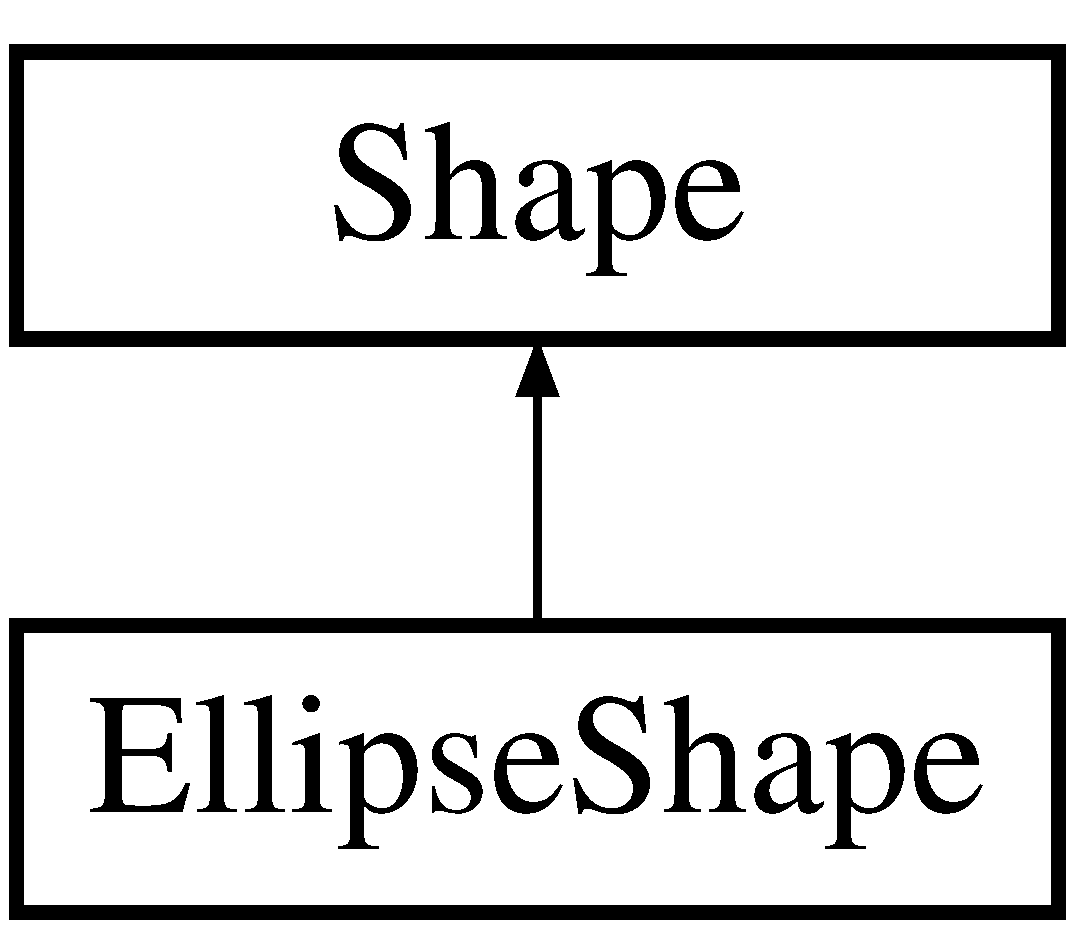
\includegraphics[height=2.000000cm]{class_ellipse_shape}
\end{center}
\end{figure}
\subsection*{Public Member Functions}
\begin{DoxyCompactItemize}
\item 
\mbox{\Hypertarget{class_ellipse_shape_a095a9119b9c505cfddd2d7a908aaa2fa}\label{class_ellipse_shape_a095a9119b9c505cfddd2d7a908aaa2fa}} 
\hyperlink{class_ellipse_shape_a095a9119b9c505cfddd2d7a908aaa2fa}{Ellipse\+Shape} (const sf\+::\+Vector2f \&radius=sf\+::\+Vector2f(0, 0), unsigned int p\+\_\+ui\+Point\+Count=50)
\begin{DoxyCompactList}\small\item\em constructor sets up the initial variables i.\+e. radius and point count \end{DoxyCompactList}\item 
\mbox{\Hypertarget{class_ellipse_shape_a7985921507ea04620ea7e2affb1871ec}\label{class_ellipse_shape_a7985921507ea04620ea7e2affb1871ec}} 
void \hyperlink{class_ellipse_shape_a7985921507ea04620ea7e2affb1871ec}{set\+Radius} (const sf\+::\+Vector2f \&radius)
\begin{DoxyCompactList}\small\item\em Radius setter. \end{DoxyCompactList}\item 
\mbox{\Hypertarget{class_ellipse_shape_a539f2728e967a2111e41e157467764c4}\label{class_ellipse_shape_a539f2728e967a2111e41e157467764c4}} 
const sf\+::\+Vector2f \& \hyperlink{class_ellipse_shape_a539f2728e967a2111e41e157467764c4}{get\+Radius} () const
\begin{DoxyCompactList}\small\item\em Radius getter. \end{DoxyCompactList}\item 
\mbox{\Hypertarget{class_ellipse_shape_ad9afe1dc2ce0e24a2af6bec2999aeb6b}\label{class_ellipse_shape_ad9afe1dc2ce0e24a2af6bec2999aeb6b}} 
virtual unsigned int \hyperlink{class_ellipse_shape_ad9afe1dc2ce0e24a2af6bec2999aeb6b}{get\+Point\+Count} () const
\begin{DoxyCompactList}\small\item\em Point count getter. \end{DoxyCompactList}\item 
\mbox{\Hypertarget{class_ellipse_shape_ab922b1ae42b7896b7d01d8d8d4759d65}\label{class_ellipse_shape_ab922b1ae42b7896b7d01d8d8d4759d65}} 
virtual sf\+::\+Vector2f \hyperlink{class_ellipse_shape_ab922b1ae42b7896b7d01d8d8d4759d65}{get\+Point} (unsigned int index) const
\begin{DoxyCompactList}\small\item\em Returns point with specified index. \end{DoxyCompactList}\end{DoxyCompactItemize}


\subsection{Detailed Description}
Custom S\+F\+ML shape class since sf\+::\+Circle cannont be scaled along the x and y axis individually. 

The documentation for this class was generated from the following file\+:\begin{DoxyCompactItemize}
\item 
D\+:/\+Sam/\+D\+M\+U/\+Year 3/\+I\+M\+A\+T3451 -\/ Final/\+Animation project repo/\+Animation Tool/\+Animation Project/include/Ellipse\+Shape.\+h\end{DoxyCompactItemize}

\hypertarget{class_event_handler}{}\section{Event\+Handler Class Reference}
\label{class_event_handler}\index{Event\+Handler@{Event\+Handler}}


Handles the connecting and registering of signals.  




{\ttfamily \#include $<$Event\+Handler.\+h$>$}

\subsection*{Public Member Functions}
\begin{DoxyCompactItemize}
\item 
\mbox{\Hypertarget{class_event_handler_a5d7ff24c664f9d1c00a417e9716471cc}\label{class_event_handler_a5d7ff24c664f9d1c00a417e9716471cc}} 
\hyperlink{class_event_handler_a5d7ff24c664f9d1c00a417e9716471cc}{Event\+Handler} (\hyperlink{class_event_handler}{Event\+Handler} const \&)=delete
\begin{DoxyCompactList}\small\item\em Copy operator. \end{DoxyCompactList}\item 
\mbox{\Hypertarget{class_event_handler_acf2df364aed9018b3f1b6c30f2e37654}\label{class_event_handler_acf2df364aed9018b3f1b6c30f2e37654}} 
\hyperlink{class_event_handler}{Event\+Handler} \& \hyperlink{class_event_handler_acf2df364aed9018b3f1b6c30f2e37654}{operator=} (\hyperlink{class_event_handler}{Event\+Handler} const \&)=delete
\begin{DoxyCompactList}\small\item\em Assignment operator. \end{DoxyCompactList}\item 
\mbox{\Hypertarget{class_event_handler_a6835697a012c284ca8ca9c32f26b8463}\label{class_event_handler_a6835697a012c284ca8ca9c32f26b8463}} 
{\footnotesize template$<$typename... Args$>$ }\\void \hyperlink{class_event_handler_a6835697a012c284ca8ca9c32f26b8463}{Register2} (std\+::string p\+\_\+\+Signal\+Name, \hyperlink{class_signal}{Signal}$<$ Args... $>$ $\ast$p\+\_\+\+Signal)
\begin{DoxyCompactList}\small\item\em Template function that can take any type of signal pointer and inserts it in the map. \end{DoxyCompactList}\item 
\mbox{\Hypertarget{class_event_handler_a53fc1f2852e49aedb4cfe766bbc80b6f}\label{class_event_handler_a53fc1f2852e49aedb4cfe766bbc80b6f}} 
{\footnotesize template$<$typename... Args$>$ }\\int \hyperlink{class_event_handler_a53fc1f2852e49aedb4cfe766bbc80b6f}{Connect2} (std\+::string p\+\_\+\+Signal\+Name, std\+::function$<$ void(Args...)$>$ const \&p\+\_\+\+Listener)
\begin{DoxyCompactList}\small\item\em Template function that can take any type of function pointer and connects it to a signal with an associated name. \end{DoxyCompactList}\item 
\mbox{\Hypertarget{class_event_handler_a76ee03c87cfebc9f2bdb4d15a1d3d3b6}\label{class_event_handler_a76ee03c87cfebc9f2bdb4d15a1d3d3b6}} 
void \hyperlink{class_event_handler_a76ee03c87cfebc9f2bdb4d15a1d3d3b6}{Disconnect} (std\+::string p\+\_\+\+Signal\+Name, unsigned int p\+\_\+\+ID)
\begin{DoxyCompactList}\small\item\em Disconnect function that disconnects a callback function with ID, p\+\_\+\+ID, from a specified signal. \end{DoxyCompactList}\end{DoxyCompactItemize}
\subsection*{Static Public Member Functions}
\begin{DoxyCompactItemize}
\item 
\mbox{\Hypertarget{class_event_handler_ace8f196c90d62a0c22a07845fc6e8ff0}\label{class_event_handler_ace8f196c90d62a0c22a07845fc6e8ff0}} 
static \hyperlink{class_event_handler}{Event\+Handler} \& {\bfseries Instance} ()
\end{DoxyCompactItemize}


\subsection{Detailed Description}
Handles the connecting and registering of signals. 

The documentation for this class was generated from the following file\+:\begin{DoxyCompactItemize}
\item 
D\+:/\+Sam/\+D\+M\+U/\+Year 3/\+I\+M\+A\+T3451 -\/ Final/\+Animation project repo/\+Animation Tool/\+Animation Project/include/Event\+Handler.\+h\end{DoxyCompactItemize}

\hypertarget{struct_frame_slot}{}\section{Frame\+Slot Struct Reference}
\label{struct_frame_slot}\index{Frame\+Slot@{Frame\+Slot}}


Struct that holds data for frame slots.  




{\ttfamily \#include $<$Time\+Line.\+h$>$}

\subsection*{Public Attributes}
\begin{DoxyCompactItemize}
\item 
\mbox{\Hypertarget{struct_frame_slot_a875d2212f5563c740c4b62877b1b3202}\label{struct_frame_slot_a875d2212f5563c740c4b62877b1b3202}} 
bool {\bfseries m\+\_\+\+Active} = false
\item 
\mbox{\Hypertarget{struct_frame_slot_a82ba39808f3cfc7a0b81d15369fc1c5e}\label{struct_frame_slot_a82ba39808f3cfc7a0b81d15369fc1c5e}} 
sf\+::\+Rectangle\+Shape {\bfseries m\+\_\+\+Rect}
\item 
\mbox{\Hypertarget{struct_frame_slot_a1d57d7133707bafbdd9293fe7019d19b}\label{struct_frame_slot_a1d57d7133707bafbdd9293fe7019d19b}} 
unsigned int {\bfseries m\+\_\+\+Key\+Frame}
\end{DoxyCompactItemize}


\subsection{Detailed Description}
Struct that holds data for frame slots. 

The documentation for this struct was generated from the following file\+:\begin{DoxyCompactItemize}
\item 
D\+:/\+Sam/\+D\+M\+U/\+Year 3/\+I\+M\+A\+T3451 -\/ Final/\+Animation project repo/\+Animation Tool/\+Animation Project/include/Time\+Line.\+h\end{DoxyCompactItemize}

\hypertarget{class_has_interaction_ptrs}{}\section{Has\+Interaction\+Ptrs Class Reference}
\label{class_has_interaction_ptrs}\index{Has\+Interaction\+Ptrs@{Has\+Interaction\+Ptrs}}


inherited by classes that need to used the interaction pointers  




{\ttfamily \#include $<$Interaction\+Ptrs.\+h$>$}

Inheritance diagram for Has\+Interaction\+Ptrs\+:\begin{figure}[H]
\begin{center}
\leavevmode
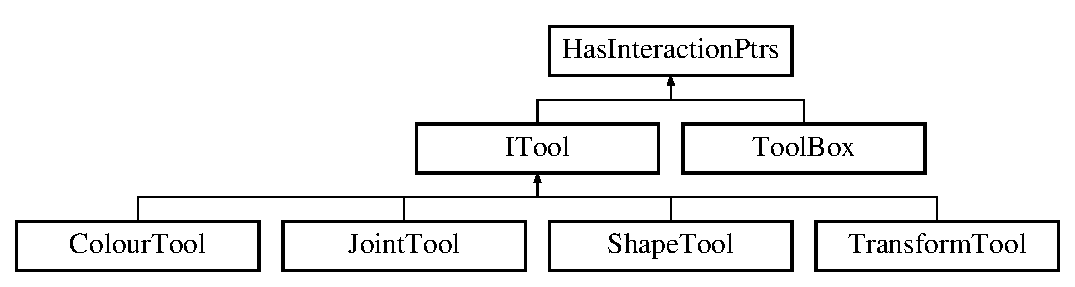
\includegraphics[height=3.000000cm]{class_has_interaction_ptrs}
\end{center}
\end{figure}
\subsection*{Public Member Functions}
\begin{DoxyCompactItemize}
\item 
\mbox{\Hypertarget{class_has_interaction_ptrs_a899e437486cacab5fbaa3cde6af80356}\label{class_has_interaction_ptrs_a899e437486cacab5fbaa3cde6af80356}} 
void \hyperlink{class_has_interaction_ptrs_a899e437486cacab5fbaa3cde6af80356}{set\+Subsystem\+Pointers} (\hyperlink{struct_interaction_ptrs}{Interaction\+Ptrs} $\ast$p\+\_\+p\+SP)
\begin{DoxyCompactList}\small\item\em Setter for m\+\_\+p\+IP. \end{DoxyCompactList}\item 
\mbox{\Hypertarget{class_has_interaction_ptrs_a2bc6b1bc6112768fbcc5c6b83c2857a3}\label{class_has_interaction_ptrs_a2bc6b1bc6112768fbcc5c6b83c2857a3}} 
\hyperlink{struct_interaction_ptrs}{Interaction\+Ptrs} $\ast$ \hyperlink{class_has_interaction_ptrs_a2bc6b1bc6112768fbcc5c6b83c2857a3}{get\+Subsystem\+Pointers} ()
\begin{DoxyCompactList}\small\item\em Returns the interaction pointer. \end{DoxyCompactList}\item 
\mbox{\Hypertarget{class_has_interaction_ptrs_ad7bb97d4ee16b015374108b6514fd02b}\label{class_has_interaction_ptrs_ad7bb97d4ee16b015374108b6514fd02b}} 
std\+::vector$<$ \hyperlink{class_object}{Object} $\ast$ $>$ $\ast$ {\bfseries get\+Objects} ()
\item 
\mbox{\Hypertarget{class_has_interaction_ptrs_a5efae28f7a0dbbaaea8e728ef5e44fcd}\label{class_has_interaction_ptrs_a5efae28f7a0dbbaaea8e728ef5e44fcd}} 
\hyperlink{class_shapes}{Shapes} $\ast$ \hyperlink{class_has_interaction_ptrs_a5efae28f7a0dbbaaea8e728ef5e44fcd}{get\+Shapes} ()
\begin{DoxyCompactList}\small\item\em Returns a pointer to the shapes container. \end{DoxyCompactList}\item 
\mbox{\Hypertarget{class_has_interaction_ptrs_ab78f0b1500beb0da994b8895831ea366}\label{class_has_interaction_ptrs_ab78f0b1500beb0da994b8895831ea366}} 
sf\+::\+Render\+Window $\ast$ \hyperlink{class_has_interaction_ptrs_ab78f0b1500beb0da994b8895831ea366}{get\+Window} ()
\begin{DoxyCompactList}\small\item\em Returns a pointer to the window. \end{DoxyCompactList}\item 
\mbox{\Hypertarget{class_has_interaction_ptrs_aacd3f410a05c5e6a15cfb18a901eac5c}\label{class_has_interaction_ptrs_aacd3f410a05c5e6a15cfb18a901eac5c}} 
\hyperlink{class_camera}{Camera} $\ast$ \hyperlink{class_has_interaction_ptrs_aacd3f410a05c5e6a15cfb18a901eac5c}{get\+Camera} ()
\begin{DoxyCompactList}\small\item\em Returns a pointer to the camera. \end{DoxyCompactList}\end{DoxyCompactItemize}
\subsection*{Protected Member Functions}
\begin{DoxyCompactItemize}
\item 
\mbox{\Hypertarget{class_has_interaction_ptrs_a44e282717a0bf39994df55b5153874a4}\label{class_has_interaction_ptrs_a44e282717a0bf39994df55b5153874a4}} 
\hyperlink{class_has_interaction_ptrs_a44e282717a0bf39994df55b5153874a4}{Has\+Interaction\+Ptrs} (\hyperlink{struct_interaction_ptrs}{Interaction\+Ptrs} $\ast$p\+\_\+p\+SP)
\begin{DoxyCompactList}\small\item\em constructor \end{DoxyCompactList}\end{DoxyCompactItemize}


\subsection{Detailed Description}
inherited by classes that need to used the interaction pointers 

The documentation for this class was generated from the following file\+:\begin{DoxyCompactItemize}
\item 
D\+:/\+Sam/\+D\+M\+U/\+Year 3/\+I\+M\+A\+T3451 -\/ Final/\+Animation project repo/\+Animation Tool/\+Animation Project/include/Interaction\+Ptrs.\+h\end{DoxyCompactItemize}

\hypertarget{struct_interaction_ptrs}{}\section{Interaction\+Ptrs Struct Reference}
\label{struct_interaction_ptrs}\index{Interaction\+Ptrs@{Interaction\+Ptrs}}


Interaction pointers struct.  




{\ttfamily \#include $<$Interaction\+Ptrs.\+h$>$}

\subsection*{Public Member Functions}
\begin{DoxyCompactItemize}
\item 
\mbox{\Hypertarget{struct_interaction_ptrs_a508c3b51f098bdf4aee1379ecf4d0c6f}\label{struct_interaction_ptrs_a508c3b51f098bdf4aee1379ecf4d0c6f}} 
\hyperlink{struct_interaction_ptrs_a508c3b51f098bdf4aee1379ecf4d0c6f}{Interaction\+Ptrs} (std\+::vector$<$ \hyperlink{class_object}{Object} $\ast$$>$ $\ast$p\+\_\+p\+Objects, \hyperlink{class_shapes}{Shapes} $\ast$p\+\_\+\+Shapes, sf\+::\+Render\+Window $\ast$p\+\_\+p\+Window, \hyperlink{class_camera}{Camera} $\ast$p\+\_\+p\+Camera)
\begin{DoxyCompactList}\small\item\em interaction pointers constructor \end{DoxyCompactList}\end{DoxyCompactItemize}
\subsection*{Public Attributes}
\begin{DoxyCompactItemize}
\item 
\mbox{\Hypertarget{struct_interaction_ptrs_af227218d0e28a40c406f8406b77d6486}\label{struct_interaction_ptrs_af227218d0e28a40c406f8406b77d6486}} 
std\+::vector$<$ \hyperlink{class_object}{Object} $\ast$ $>$ $\ast$ {\bfseries m\+\_\+p\+Objects}
\item 
\mbox{\Hypertarget{struct_interaction_ptrs_ae55ba8e8bd18a67eae5740b76c6b3791}\label{struct_interaction_ptrs_ae55ba8e8bd18a67eae5740b76c6b3791}} 
\hyperlink{class_shapes}{Shapes} $\ast$ \hyperlink{struct_interaction_ptrs_ae55ba8e8bd18a67eae5740b76c6b3791}{m\+\_\+\+Shapes}
\begin{DoxyCompactList}\small\item\em shapes container used to create and interact with shapes \end{DoxyCompactList}\item 
\mbox{\Hypertarget{struct_interaction_ptrs_a9ef141a4721b7420290ed85011eb4e29}\label{struct_interaction_ptrs_a9ef141a4721b7420290ed85011eb4e29}} 
sf\+::\+Render\+Window $\ast$ \hyperlink{struct_interaction_ptrs_a9ef141a4721b7420290ed85011eb4e29}{m\+\_\+p\+Window}
\begin{DoxyCompactList}\small\item\em pointer to the window \end{DoxyCompactList}\item 
\mbox{\Hypertarget{struct_interaction_ptrs_a1c0387f28c3d217ad2b7d30fef015b50}\label{struct_interaction_ptrs_a1c0387f28c3d217ad2b7d30fef015b50}} 
\hyperlink{class_camera}{Camera} $\ast$ \hyperlink{struct_interaction_ptrs_a1c0387f28c3d217ad2b7d30fef015b50}{m\+\_\+p\+Camera}
\begin{DoxyCompactList}\small\item\em pointer to the camera view \end{DoxyCompactList}\end{DoxyCompactItemize}


\subsection{Detailed Description}
Interaction pointers struct. 

The documentation for this struct was generated from the following file\+:\begin{DoxyCompactItemize}
\item 
D\+:/\+Sam/\+D\+M\+U/\+Year 3/\+I\+M\+A\+T3451 -\/ Final/\+Animation project repo/\+Animation Tool/\+Animation Project/include/Interaction\+Ptrs.\+h\end{DoxyCompactItemize}

\hypertarget{class_interpolation_helper}{}\section{Interpolation\+Helper Class Reference}
\label{class_interpolation_helper}\index{Interpolation\+Helper@{Interpolation\+Helper}}


Contains methods for interplating between two positions.  




{\ttfamily \#include $<$Interpolation\+Helper.\+h$>$}

\subsection*{Public Member Functions}
\begin{DoxyCompactItemize}
\item 
\mbox{\Hypertarget{class_interpolation_helper_aa2fba4f6c109fd6541e9fce8729d469f}\label{class_interpolation_helper_aa2fba4f6c109fd6541e9fce8729d469f}} 
sf\+::\+Vector2f \hyperlink{class_interpolation_helper_aa2fba4f6c109fd6541e9fce8729d469f}{Linear} (float p\+\_\+\+Progress, sf\+::\+Vector2f p\+\_\+\+Prev, sf\+::\+Vector2f)
\begin{DoxyCompactList}\small\item\em Linear interpolation solver. \end{DoxyCompactList}\end{DoxyCompactItemize}


\subsection{Detailed Description}
Contains methods for interplating between two positions. 

The documentation for this class was generated from the following files\+:\begin{DoxyCompactItemize}
\item 
D\+:/\+Sam/\+D\+M\+U/\+Year 3/\+I\+M\+A\+T3451 -\/ Final/\+Animation project repo/\+Animation Tool/\+Animation Project/include/Interpolation\+Helper.\+h\item 
D\+:/\+Sam/\+D\+M\+U/\+Year 3/\+I\+M\+A\+T3451 -\/ Final/\+Animation project repo/\+Animation Tool/\+Animation Project/include/Interpolation\+Helper.\+cpp\end{DoxyCompactItemize}

\hypertarget{class_i_tool}{}\section{I\+Tool Class Reference}
\label{class_i_tool}\index{I\+Tool@{I\+Tool}}


handles generic methods that tools might need to use  




{\ttfamily \#include $<$I\+Tool.\+h$>$}

Inheritance diagram for I\+Tool\+:\begin{figure}[H]
\begin{center}
\leavevmode
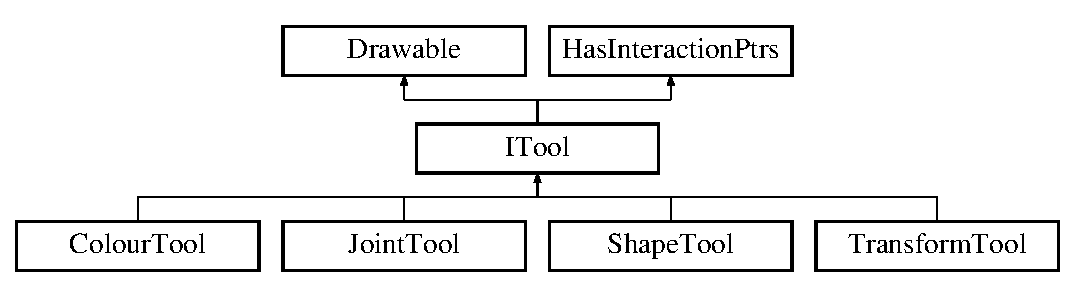
\includegraphics[height=3.000000cm]{class_i_tool}
\end{center}
\end{figure}
\subsection*{Public Member Functions}
\begin{DoxyCompactItemize}
\item 
\mbox{\Hypertarget{class_i_tool_aaee4d261cdadf0bab515ae3d0ad9fe86}\label{class_i_tool_aaee4d261cdadf0bab515ae3d0ad9fe86}} 
virtual void \hyperlink{class_i_tool_aaee4d261cdadf0bab515ae3d0ad9fe86}{Update} (float p\+\_\+\+Delta\+Time)=0
\begin{DoxyCompactList}\small\item\em Update method. \end{DoxyCompactList}\item 
\mbox{\Hypertarget{class_i_tool_a1af006baeba70bb9d2a77655e5f43827}\label{class_i_tool_a1af006baeba70bb9d2a77655e5f43827}} 
virtual void \hyperlink{class_i_tool_a1af006baeba70bb9d2a77655e5f43827}{On\+Mouse\+Click} (sf\+::\+Mouse\+::\+Button p\+\_\+\+Button, bool p\+\_\+b\+State)
\begin{DoxyCompactList}\small\item\em Callback for mouse click events. \end{DoxyCompactList}\item 
\mbox{\Hypertarget{class_i_tool_a650ec05672cd537ef7fd68f220fa9569}\label{class_i_tool_a650ec05672cd537ef7fd68f220fa9569}} 
virtual void \hyperlink{class_i_tool_a650ec05672cd537ef7fd68f220fa9569}{On\+Mouse\+Move} (sf\+::\+Vector2i p\+\_\+\+Mouse\+Window\+Pos, sf\+::\+Vector2f p\+\_\+\+Mouse\+Canvas\+Pos)
\begin{DoxyCompactList}\small\item\em callback for mouse move events \end{DoxyCompactList}\item 
\mbox{\Hypertarget{class_i_tool_aa48cc732ed27ccbbaf4731aee956e959}\label{class_i_tool_aa48cc732ed27ccbbaf4731aee956e959}} 
virtual void \hyperlink{class_i_tool_aa48cc732ed27ccbbaf4731aee956e959}{draw} (sf\+::\+Render\+Target \&target, sf\+::\+Render\+States states) const
\begin{DoxyCompactList}\small\item\em draw method \end{DoxyCompactList}\end{DoxyCompactItemize}
\subsection*{Public Attributes}
\begin{DoxyCompactItemize}
\item 
\mbox{\Hypertarget{class_i_tool_a899ebf4a35a3ba0d6933db8e07f075bc}\label{class_i_tool_a899ebf4a35a3ba0d6933db8e07f075bc}} 
bool \hyperlink{class_i_tool_a899ebf4a35a3ba0d6933db8e07f075bc}{m\+\_\+\+Active} = false
\begin{DoxyCompactList}\small\item\em Is the tool active. \end{DoxyCompactList}\end{DoxyCompactItemize}
\subsection*{Protected Member Functions}
\begin{DoxyCompactItemize}
\item 
\mbox{\Hypertarget{class_i_tool_a79901d47b06c21ac66ae4b5dea63a72d}\label{class_i_tool_a79901d47b06c21ac66ae4b5dea63a72d}} 
\hyperlink{class_i_tool_a79901d47b06c21ac66ae4b5dea63a72d}{I\+Tool} (\hyperlink{struct_interaction_ptrs}{Interaction\+Ptrs} $\ast$p\+\_\+p\+SP)
\begin{DoxyCompactList}\small\item\em Constructor handles the inraction pointer giving it to the constructor of \hyperlink{class_has_interaction_ptrs}{Has\+Interaction\+Ptrs}. \end{DoxyCompactList}\end{DoxyCompactItemize}
\subsection*{Protected Attributes}
\begin{DoxyCompactItemize}
\item 
\mbox{\Hypertarget{class_i_tool_af99caebe9dc3aa965571408f20be0749}\label{class_i_tool_af99caebe9dc3aa965571408f20be0749}} 
sf\+::\+Vector2f \hyperlink{class_i_tool_af99caebe9dc3aa965571408f20be0749}{m\+\_\+\+Mouse\+Canvas\+Pos}
\begin{DoxyCompactList}\small\item\em The mouse position on the canvas. \end{DoxyCompactList}\item 
\mbox{\Hypertarget{class_i_tool_a5231eb512a418f4e621f23d0c7fb4c6e}\label{class_i_tool_a5231eb512a418f4e621f23d0c7fb4c6e}} 
sf\+::\+Vector2i \hyperlink{class_i_tool_a5231eb512a418f4e621f23d0c7fb4c6e}{m\+\_\+\+Mouse\+Window\+Pos}
\begin{DoxyCompactList}\small\item\em The mouse position on the window. \end{DoxyCompactList}\end{DoxyCompactItemize}


\subsection{Detailed Description}
handles generic methods that tools might need to use 

The documentation for this class was generated from the following file\+:\begin{DoxyCompactItemize}
\item 
D\+:/\+Sam/\+D\+M\+U/\+Year 3/\+I\+M\+A\+T3451 -\/ Final/\+Animation project repo/\+Animation Tool/\+Animation Project/include/I\+Tool.\+h\end{DoxyCompactItemize}

\hypertarget{class_joint_tool}{}\section{Joint\+Tool Class Reference}
\label{class_joint_tool}\index{Joint\+Tool@{Joint\+Tool}}


Handles the linking joints between objest.  




{\ttfamily \#include $<$Joint\+Tool.\+h$>$}

Inheritance diagram for Joint\+Tool\+:\begin{figure}[H]
\begin{center}
\leavevmode
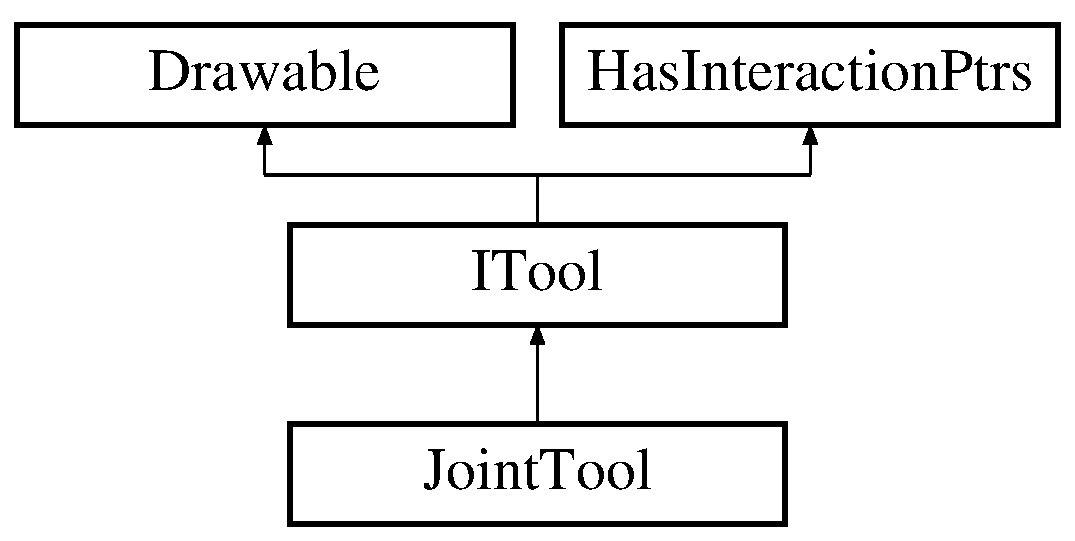
\includegraphics[height=3.000000cm]{class_joint_tool}
\end{center}
\end{figure}
\subsection*{Public Member Functions}
\begin{DoxyCompactItemize}
\item 
\mbox{\Hypertarget{class_joint_tool_a023c782f823a670bc230a437eff95a6d}\label{class_joint_tool_a023c782f823a670bc230a437eff95a6d}} 
\hyperlink{class_joint_tool_a023c782f823a670bc230a437eff95a6d}{Joint\+Tool} (\hyperlink{struct_interaction_ptrs}{Interaction\+Ptrs} $\ast$p\+\_\+p\+SP)
\begin{DoxyCompactList}\small\item\em Constructor. \end{DoxyCompactList}\item 
\mbox{\Hypertarget{class_joint_tool_ac00895518431be66662033b126ae6427}\label{class_joint_tool_ac00895518431be66662033b126ae6427}} 
void \hyperlink{class_joint_tool_ac00895518431be66662033b126ae6427}{Update} (float p\+\_\+\+Delta\+Time) override
\begin{DoxyCompactList}\small\item\em Updates the joint line during a selection. \end{DoxyCompactList}\item 
\mbox{\Hypertarget{class_joint_tool_a1d67646dea85f21555baa3dffc884876}\label{class_joint_tool_a1d67646dea85f21555baa3dffc884876}} 
void \hyperlink{class_joint_tool_a1d67646dea85f21555baa3dffc884876}{On\+Mouse\+Click} (sf\+::\+Mouse\+::\+Button p\+\_\+\+Button, bool p\+\_\+b\+State) override
\begin{DoxyCompactList}\small\item\em callback for mouse click events used to determine the parent and child of a joint \end{DoxyCompactList}\item 
\mbox{\Hypertarget{class_joint_tool_afc73a29a1c72a5e58da7d8f2cc6d43b4}\label{class_joint_tool_afc73a29a1c72a5e58da7d8f2cc6d43b4}} 
void \hyperlink{class_joint_tool_afc73a29a1c72a5e58da7d8f2cc6d43b4}{draw} (sf\+::\+Render\+Target \&target, sf\+::\+Render\+States states) const
\begin{DoxyCompactList}\small\item\em Draw the joint line. \end{DoxyCompactList}\end{DoxyCompactItemize}
\subsection*{Additional Inherited Members}


\subsection{Detailed Description}
Handles the linking joints between objest. 

The documentation for this class was generated from the following file\+:\begin{DoxyCompactItemize}
\item 
D\+:/\+Sam/\+D\+M\+U/\+Year 3/\+I\+M\+A\+T3451 -\/ Final/\+Animation project repo/\+Animation Tool/\+Animation Project/include/Joint\+Tool.\+h\end{DoxyCompactItemize}

\hypertarget{struct_key_frame}{}\section{Key\+Frame Struct Reference}
\label{struct_key_frame}\index{Key\+Frame@{Key\+Frame}}


Struct that holds frame number and its corresponding object data.  




{\ttfamily \#include $<$Anim\+Structs.\+h$>$}

\subsection*{Public Attributes}
\begin{DoxyCompactItemize}
\item 
\mbox{\Hypertarget{struct_key_frame_accd5dd8cf11311d70e84138329fb0e9e}\label{struct_key_frame_accd5dd8cf11311d70e84138329fb0e9e}} 
unsigned int {\bfseries m\+\_\+\+Frame}
\item 
\mbox{\Hypertarget{struct_key_frame_a221a8068b554fdfba1df906d1204f019}\label{struct_key_frame_a221a8068b554fdfba1df906d1204f019}} 
\hyperlink{class_object_data}{Object\+Data} {\bfseries m\+\_\+\+Object\+Data}
\end{DoxyCompactItemize}


\subsection{Detailed Description}
Struct that holds frame number and its corresponding object data. 

The documentation for this struct was generated from the following file\+:\begin{DoxyCompactItemize}
\item 
D\+:/\+Sam/\+D\+M\+U/\+Year 3/\+I\+M\+A\+T3451 -\/ Final/\+Animation project repo/\+Animation Tool/\+Animation Project/include/Anim\+Structs.\+h\end{DoxyCompactItemize}

\hypertarget{class_keyframe_manager}{}\section{Keyframe\+Manager Class Reference}
\label{class_keyframe_manager}\index{Keyframe\+Manager@{Keyframe\+Manager}}


Manages keyframe data for objects Provides functionality to save, load, iterate and interpolate between keyframes.  




{\ttfamily \#include $<$Keyframe\+Manager.\+h$>$}

\subsection*{Public Member Functions}
\begin{DoxyCompactItemize}
\item 
\mbox{\Hypertarget{class_keyframe_manager_aeb89db344dcdca1c212b8e9f8d75a024}\label{class_keyframe_manager_aeb89db344dcdca1c212b8e9f8d75a024}} 
\hyperlink{class_keyframe_manager_aeb89db344dcdca1c212b8e9f8d75a024}{Keyframe\+Manager} (unsigned int p\+\_\+\+Frame\+Rate, double p\+\_\+\+Animation\+Time, \hyperlink{class_shapes}{Shapes} $\ast$p\+\_\+\+Shapes)
\begin{DoxyCompactList}\small\item\em Constructor that takes framerate, runtime and a pointer to the shapes manager. \end{DoxyCompactList}\item 
\mbox{\Hypertarget{class_keyframe_manager_a53c98866dce1a595c6e289e028234e99}\label{class_keyframe_manager_a53c98866dce1a595c6e289e028234e99}} 
void \hyperlink{class_keyframe_manager_a53c98866dce1a595c6e289e028234e99}{Record\+Keyframe} (unsigned int p\+\_\+\+ID)
\begin{DoxyCompactList}\small\item\em Record a keyframe at the current frame number for shape with given ID. \end{DoxyCompactList}\item 
\mbox{\Hypertarget{class_keyframe_manager_acfa120e0e5ea6df1724c4191bf32c503}\label{class_keyframe_manager_acfa120e0e5ea6df1724c4191bf32c503}} 
void \hyperlink{class_keyframe_manager_acfa120e0e5ea6df1724c4191bf32c503}{Delete\+Keyframe} (unsigned int p\+\_\+\+ID, unsigned int p\+\_\+\+Frame\+Number)
\begin{DoxyCompactList}\small\item\em Delete the keyframe of shape with ID at frame p\+\_\+\+Frame\+Number. \end{DoxyCompactList}\item 
\mbox{\Hypertarget{class_keyframe_manager_a6dd869e79b4e4be340abf62db07c21ae}\label{class_keyframe_manager_a6dd869e79b4e4be340abf62db07c21ae}} 
void \hyperlink{class_keyframe_manager_a6dd869e79b4e4be340abf62db07c21ae}{Set\+Current\+Frame} (unsigned int p\+\_\+\+Frame\+Number)
\begin{DoxyCompactList}\small\item\em Sets the current frame to p\+\_\+\+Frame\+Number and places shapes at their interpolated positions. \end{DoxyCompactList}\item 
\mbox{\Hypertarget{class_keyframe_manager_a38d18fb54e65492a3682b865c3cf6b53}\label{class_keyframe_manager_a38d18fb54e65492a3682b865c3cf6b53}} 
void \hyperlink{class_keyframe_manager_a38d18fb54e65492a3682b865c3cf6b53}{Play} ()
\begin{DoxyCompactList}\small\item\em Sets the animation state to playing. \end{DoxyCompactList}\item 
\mbox{\Hypertarget{class_keyframe_manager_a2ca51f9d58c2c346b5cda13ab13f3675}\label{class_keyframe_manager_a2ca51f9d58c2c346b5cda13ab13f3675}} 
void \hyperlink{class_keyframe_manager_a2ca51f9d58c2c346b5cda13ab13f3675}{Stop} ()
\begin{DoxyCompactList}\small\item\em Sets the animation state to stopped. \end{DoxyCompactList}\item 
\mbox{\Hypertarget{class_keyframe_manager_affb43ea87dcd581a8938238e275cf1bf}\label{class_keyframe_manager_affb43ea87dcd581a8938238e275cf1bf}} 
void \hyperlink{class_keyframe_manager_affb43ea87dcd581a8938238e275cf1bf}{Update} ()
\begin{DoxyCompactList}\small\item\em Updates the animation by calling \char`\"{}\+Set\+Current\+Frame\char`\"{} every update frame if the animation state is set to \char`\"{}\+Playing\char`\"{}. \end{DoxyCompactList}\item 
\mbox{\Hypertarget{class_keyframe_manager_ac94f8f3d7a9c65ee226df806e81d0a90}\label{class_keyframe_manager_ac94f8f3d7a9c65ee226df806e81d0a90}} 
unsigned int \hyperlink{class_keyframe_manager_ac94f8f3d7a9c65ee226df806e81d0a90}{Get\+Total\+Frames} ()
\begin{DoxyCompactList}\small\item\em Returns the total frame number. \end{DoxyCompactList}\item 
\mbox{\Hypertarget{class_keyframe_manager_a5aa8a4aba82178223ab869ff3bad0dd3}\label{class_keyframe_manager_a5aa8a4aba82178223ab869ff3bad0dd3}} 
unsigned int \hyperlink{class_keyframe_manager_a5aa8a4aba82178223ab869ff3bad0dd3}{Get\+Current\+Frame} ()
\begin{DoxyCompactList}\small\item\em Returns the current frame number. \end{DoxyCompactList}\end{DoxyCompactItemize}
\subsection*{Public Attributes}
\begin{DoxyCompactItemize}
\item 
\mbox{\Hypertarget{class_keyframe_manager_a63db1d456f6f73bfc756583ac9ff6b2b}\label{class_keyframe_manager_a63db1d456f6f73bfc756583ac9ff6b2b}} 
\hyperlink{class_signal}{Signal}$<$ const flat\+\_\+set$<$ \hyperlink{struct_shape_key_frames}{Shape\+Key\+Frames}, \hyperlink{struct_compare_id}{Compare\+Id} $>$ \&, Frame\+State $>$ \hyperlink{class_keyframe_manager_a63db1d456f6f73bfc756583ac9ff6b2b}{On\+Update}
\begin{DoxyCompactList}\small\item\em \hyperlink{class_signal}{Signal} that gives out the animation data to anything that needs it. \end{DoxyCompactList}\end{DoxyCompactItemize}


\subsection{Detailed Description}
Manages keyframe data for objects Provides functionality to save, load, iterate and interpolate between keyframes. 

The documentation for this class was generated from the following file\+:\begin{DoxyCompactItemize}
\item 
D\+:/\+Sam/\+D\+M\+U/\+Year 3/\+I\+M\+A\+T3451 -\/ Final/\+Animation project repo/\+Animation Tool/\+Animation Project/include/Keyframe\+Manager.\+h\end{DoxyCompactItemize}

\hypertarget{class_object}{}\section{Object Class Reference}
\label{class_object}\index{Object@{Object}}


Handles a quadpart and polyshape to make up a more transformable object that just using an S\+F\+ML shape.  




{\ttfamily \#include $<$Object.\+h$>$}

Inheritance diagram for Object\+:\begin{figure}[H]
\begin{center}
\leavevmode
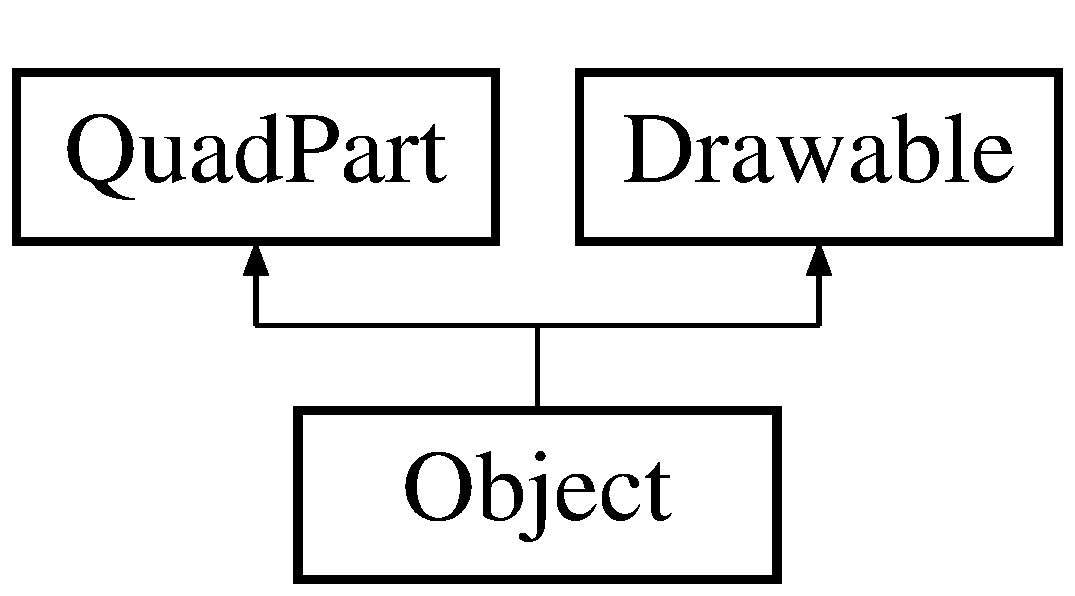
\includegraphics[height=2.000000cm]{class_object}
\end{center}
\end{figure}
\subsection*{Public Member Functions}
\begin{DoxyCompactItemize}
\item 
\mbox{\Hypertarget{class_object_ae240ad6fec4239f2d631cefacd7fd8dd}\label{class_object_ae240ad6fec4239f2d631cefacd7fd8dd}} 
\hyperlink{class_object_ae240ad6fec4239f2d631cefacd7fd8dd}{Object} (Shape\+Type p\+\_\+e\+Shape\+Type)
\begin{DoxyCompactList}\small\item\em Constructor that takes just a shape type enum. \end{DoxyCompactList}\item 
\mbox{\Hypertarget{class_object_ae525cdbb73d2ca88dd5c9422405744d4}\label{class_object_ae525cdbb73d2ca88dd5c9422405744d4}} 
\hyperlink{class_object_ae525cdbb73d2ca88dd5c9422405744d4}{Object} (Shape\+Type p\+\_\+e\+Shape\+Type, sf\+::\+Vector2f p\+\_\+\+Pos, sf\+::\+Vector2f p\+\_\+\+Size)
\begin{DoxyCompactList}\small\item\em Constructor that thake shape type, position and size. \end{DoxyCompactList}\item 
\mbox{\Hypertarget{class_object_a50cf60a49f4c109a63b8ba2a802d24c3}\label{class_object_a50cf60a49f4c109a63b8ba2a802d24c3}} 
\hyperlink{class_object_a50cf60a49f4c109a63b8ba2a802d24c3}{Object} (Shape\+Type p\+\_\+e\+Shape\+Type, sf\+::\+Vector2f p\+\_\+\+Pos, sf\+::\+Vector2f p\+\_\+\+Size, unsigned int p\+\_\+ui\+Point\+Count)
\begin{DoxyCompactList}\small\item\em Constructor that takes shape type, position, size and point count. \end{DoxyCompactList}\item 
\mbox{\Hypertarget{class_object_adec6108282a005f78653c7b53931167f}\label{class_object_adec6108282a005f78653c7b53931167f}} 
\hyperlink{class_object_adec6108282a005f78653c7b53931167f}{Object} (const \hyperlink{class_object}{Object} \&p\+\_\+\+Other)
\begin{DoxyCompactList}\small\item\em \hyperlink{class_object}{Object} copy constructor overload. \end{DoxyCompactList}\item 
\mbox{\Hypertarget{class_object_aa904f948ec72f2cbec99a9eee5ed387e}\label{class_object_aa904f948ec72f2cbec99a9eee5ed387e}} 
void \hyperlink{class_object_aa904f948ec72f2cbec99a9eee5ed387e}{operator=} (const \hyperlink{class_object}{Object} \&p\+\_\+\+Other)
\begin{DoxyCompactList}\small\item\em \hyperlink{class_object}{Object} assignment operator overload that prevents polyshape becoming invalid. \end{DoxyCompactList}\item 
\mbox{\Hypertarget{class_object_a94582e86bced7fdfebc0d419a2012272}\label{class_object_a94582e86bced7fdfebc0d419a2012272}} 
void \hyperlink{class_object_a94582e86bced7fdfebc0d419a2012272}{Update\+Shape} ()
\begin{DoxyCompactList}\small\item\em Update the polyshape to match the quadpart shape. \end{DoxyCompactList}\item 
\mbox{\Hypertarget{class_object_a6c3dc18899c7d428b35b88b1474778d0}\label{class_object_a6c3dc18899c7d428b35b88b1474778d0}} 
void \hyperlink{class_object_a6c3dc18899c7d428b35b88b1474778d0}{draw} (sf\+::\+Render\+Target \&target, sf\+::\+Render\+States states) const
\begin{DoxyCompactList}\small\item\em Draw the polyshape. \end{DoxyCompactList}\end{DoxyCompactItemize}
\subsection*{Public Attributes}
\begin{DoxyCompactItemize}
\item 
\mbox{\Hypertarget{class_object_a6f8024417f011eba14377d64b39baad4}\label{class_object_a6f8024417f011eba14377d64b39baad4}} 
sf\+::\+Shape $\ast$ \hyperlink{class_object_a6f8024417f011eba14377d64b39baad4}{m\+\_\+p\+Poly\+Shape}
\begin{DoxyCompactList}\small\item\em The polymorphic sfml shape pointer. \end{DoxyCompactList}\item 
\mbox{\Hypertarget{class_object_a90cb6e9ab5acccc06a2fa2bbc9ccf793}\label{class_object_a90cb6e9ab5acccc06a2fa2bbc9ccf793}} 
std\+::string \hyperlink{class_object_a90cb6e9ab5acccc06a2fa2bbc9ccf793}{m\+\_\+\+Name}
\begin{DoxyCompactList}\small\item\em Name associated with this object (not yet used) \end{DoxyCompactList}\end{DoxyCompactItemize}
\subsection*{Additional Inherited Members}


\subsection{Detailed Description}
Handles a quadpart and polyshape to make up a more transformable object that just using an S\+F\+ML shape. 

The documentation for this class was generated from the following file\+:\begin{DoxyCompactItemize}
\item 
D\+:/\+Sam/\+D\+M\+U/\+Year 3/\+I\+M\+A\+T3451 -\/ Final/\+Animation project repo/\+Animation Tool/\+Animation Project/include/Object.\+h\end{DoxyCompactItemize}

\hypertarget{class_object_data}{}\section{Object\+Data Class Reference}
\label{class_object_data}\index{Object\+Data@{Object\+Data}}


Struct that holds object data i.\+e. position, rotation and vertices.  




{\ttfamily \#include $<$Object\+Data.\+h$>$}

\subsection*{Public Attributes}
\begin{DoxyCompactItemize}
\item 
\mbox{\Hypertarget{class_object_data_a3c0fcd774b50938d0b4c693f08437c29}\label{class_object_data_a3c0fcd774b50938d0b4c693f08437c29}} 
float {\bfseries m\+\_\+\+Rotation}
\item 
\mbox{\Hypertarget{class_object_data_aaf6c38e34f3ebfab203c06e44b870011}\label{class_object_data_aaf6c38e34f3ebfab203c06e44b870011}} 
sf\+::\+Vector2f {\bfseries m\+\_\+\+Position}
\item 
\mbox{\Hypertarget{class_object_data_aaec2ade9eff5eea0c57c6b2165f42a0e}\label{class_object_data_aaec2ade9eff5eea0c57c6b2165f42a0e}} 
std\+::vector$<$ sf\+::\+Vector2f $>$ {\bfseries m\+\_\+\+Vertices}
\end{DoxyCompactItemize}


\subsection{Detailed Description}
Struct that holds object data i.\+e. position, rotation and vertices. 

The documentation for this class was generated from the following file\+:\begin{DoxyCompactItemize}
\item 
D\+:/\+Sam/\+D\+M\+U/\+Year 3/\+I\+M\+A\+T3451 -\/ Final/\+Animation project repo/\+Animation Tool/\+Animation Project/include/Object\+Data.\+h\end{DoxyCompactItemize}

\hypertarget{class_quad_part}{}\section{Quad\+Part Class Reference}
\label{class_quad_part}\index{Quad\+Part@{Quad\+Part}}


A class that can handle more complex transformations and store joint data Made from a basic vertex array to allow for more precise transformations than that of an S\+F\+ML shape.  




{\ttfamily \#include $<$Quad\+Part.\+h$>$}

Inheritance diagram for Quad\+Part\+:\begin{figure}[H]
\begin{center}
\leavevmode
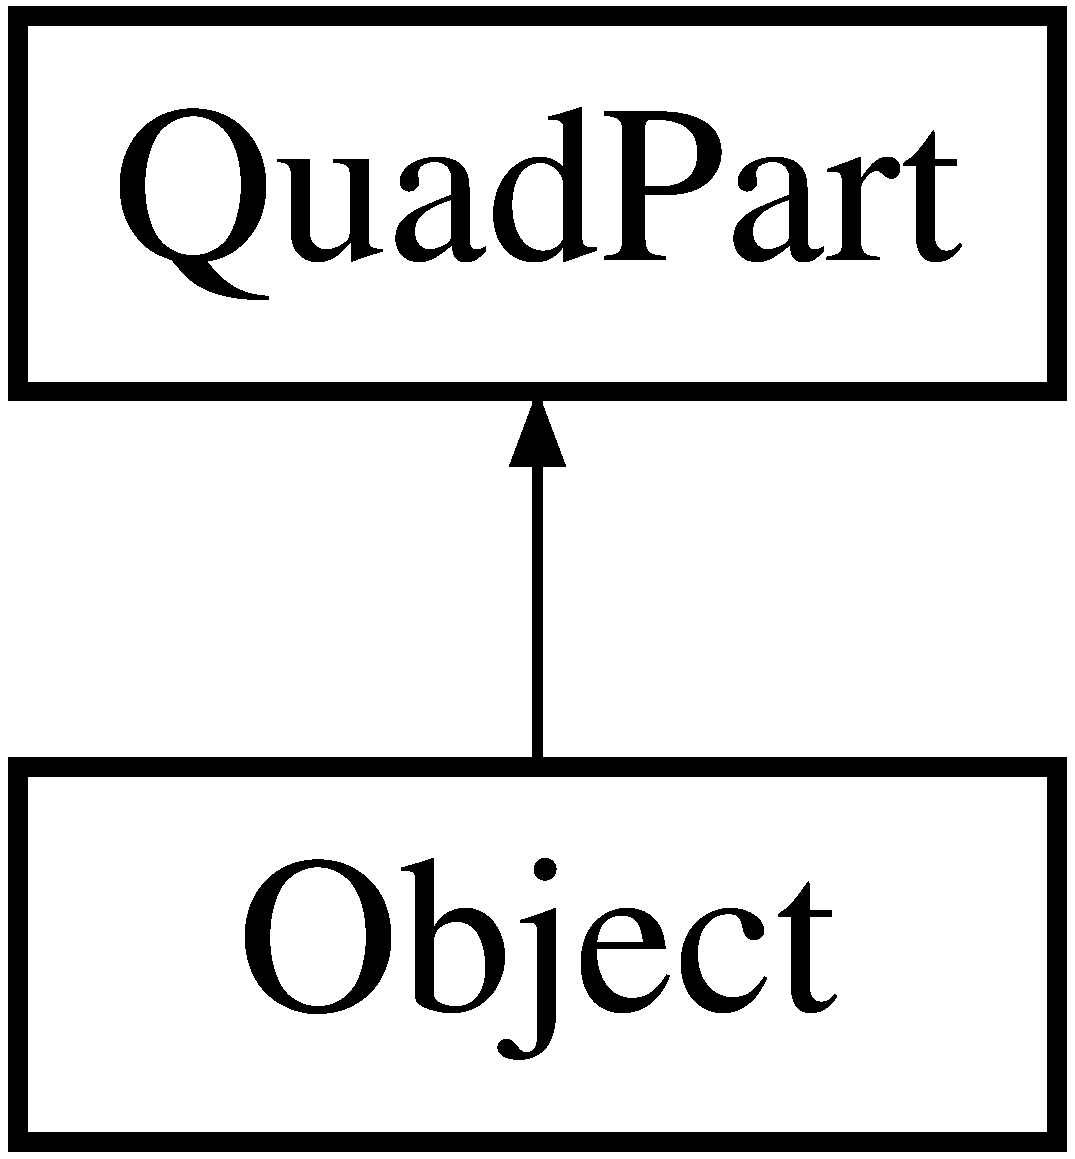
\includegraphics[height=2.000000cm]{class_quad_part}
\end{center}
\end{figure}
\subsection*{Public Member Functions}
\begin{DoxyCompactItemize}
\item 
\mbox{\Hypertarget{class_quad_part_a953ac1358c8bdd586bb477a02d42434f}\label{class_quad_part_a953ac1358c8bdd586bb477a02d42434f}} 
\hyperlink{class_quad_part_a953ac1358c8bdd586bb477a02d42434f}{Quad\+Part} ()
\begin{DoxyCompactList}\small\item\em Defualt constructor. \end{DoxyCompactList}\item 
\mbox{\Hypertarget{class_quad_part_a20fce309e6b74fc24d04f6cee536600a}\label{class_quad_part_a20fce309e6b74fc24d04f6cee536600a}} 
\hyperlink{class_quad_part_a20fce309e6b74fc24d04f6cee536600a}{Quad\+Part} (sf\+::\+Vector2f p\+\_\+\+Pos, sf\+::\+Vector2f p\+\_\+\+Size)
\begin{DoxyCompactList}\small\item\em Constructor the sets the position and size. \end{DoxyCompactList}\item 
\mbox{\Hypertarget{class_quad_part_ac4f581071de7de0dff0a757a958f67d8}\label{class_quad_part_ac4f581071de7de0dff0a757a958f67d8}} 
void \hyperlink{class_quad_part_ac4f581071de7de0dff0a757a958f67d8}{Set\+Origin} (sf\+::\+Vector2f p\+\_\+\+Pos)
\begin{DoxyCompactList}\small\item\em Method for setting the origin (only moves the position vector2f) \end{DoxyCompactList}\item 
void \hyperlink{class_quad_part_abd2f83c6c31cb1a05c97bc5711a22564}{Re\+Size} (sf\+::\+Vector2f p\+\_\+\+Offset, unsigned int p\+\_\+i\+Handle)
\item 
\mbox{\Hypertarget{class_quad_part_a7bd2f2bdb282afb965cc54847c6edfec}\label{class_quad_part_a7bd2f2bdb282afb965cc54847c6edfec}} 
void \hyperlink{class_quad_part_a7bd2f2bdb282afb965cc54847c6edfec}{Move} (sf\+::\+Vector2f p\+\_\+\+Offset)
\begin{DoxyCompactList}\small\item\em Moves the position and the vertices by an offset. \end{DoxyCompactList}\item 
\mbox{\Hypertarget{class_quad_part_ae93071d8999ff84fb5a428c21ba0056b}\label{class_quad_part_ae93071d8999ff84fb5a428c21ba0056b}} 
void \hyperlink{class_quad_part_ae93071d8999ff84fb5a428c21ba0056b}{Rotate} (float p\+\_\+\+Offset)
\begin{DoxyCompactList}\small\item\em Method that rotates the shape by an offset. \end{DoxyCompactList}\item 
\mbox{\Hypertarget{class_quad_part_a21cd672702cbe804d4d836100aa3364f}\label{class_quad_part_a21cd672702cbe804d4d836100aa3364f}} 
void \hyperlink{class_quad_part_a21cd672702cbe804d4d836100aa3364f}{Set\+Position} (sf\+::\+Vector2f p\+\_\+\+Pos)
\begin{DoxyCompactList}\small\item\em Method for setting the position of the quadpart, this includes the vertices. \end{DoxyCompactList}\item 
\mbox{\Hypertarget{class_quad_part_a81263369e0fef805b7bf9f2f0358ef16}\label{class_quad_part_a81263369e0fef805b7bf9f2f0358ef16}} 
void \hyperlink{class_quad_part_a81263369e0fef805b7bf9f2f0358ef16}{Set\+Rotation} (float p\+\_\+\+Angle)
\begin{DoxyCompactList}\small\item\em Method for setting the rotation at a given angle. \end{DoxyCompactList}\item 
\mbox{\Hypertarget{class_quad_part_a5fdd5de2794207b95d573744de8f1837}\label{class_quad_part_a5fdd5de2794207b95d573744de8f1837}} 
sf\+::\+Vector2f \hyperlink{class_quad_part_a5fdd5de2794207b95d573744de8f1837}{Get\+Position} ()
\begin{DoxyCompactList}\small\item\em Returns the positon. \end{DoxyCompactList}\item 
\mbox{\Hypertarget{class_quad_part_ad6b073d0b128af590944337a2a01d2b3}\label{class_quad_part_ad6b073d0b128af590944337a2a01d2b3}} 
float \hyperlink{class_quad_part_ad6b073d0b128af590944337a2a01d2b3}{Get\+Rotation} ()
\begin{DoxyCompactList}\small\item\em Returns the rotation. \end{DoxyCompactList}\item 
\mbox{\Hypertarget{class_quad_part_acd1a5f5d8d9a780208be5b75b1900d3c}\label{class_quad_part_acd1a5f5d8d9a780208be5b75b1900d3c}} 
sf\+::\+Vector2f \hyperlink{class_quad_part_acd1a5f5d8d9a780208be5b75b1900d3c}{Get\+Vertex} (unsigned int p\+\_\+\+Vertex)
\begin{DoxyCompactList}\small\item\em Returns one of the four vertices. \end{DoxyCompactList}\item 
\mbox{\Hypertarget{class_quad_part_a978cb59cb2c4e3407421cef33f8f02d3}\label{class_quad_part_a978cb59cb2c4e3407421cef33f8f02d3}} 
sf\+::\+Vector2f \hyperlink{class_quad_part_a978cb59cb2c4e3407421cef33f8f02d3}{Get\+Vertex8} (unsigned int p\+\_\+\+Vertex)
\begin{DoxyCompactList}\small\item\em Returns one of the four vertices or four middle points of each side. \end{DoxyCompactList}\item 
\mbox{\Hypertarget{class_quad_part_af2fa5ea599fa1f615594ff7de7914b2f}\label{class_quad_part_af2fa5ea599fa1f615594ff7de7914b2f}} 
sf\+::\+Vector2f \hyperlink{class_quad_part_af2fa5ea599fa1f615594ff7de7914b2f}{Get\+Size} ()
\begin{DoxyCompactList}\small\item\em Returns the size of the shape determined by the axis aligned vertices. \end{DoxyCompactList}\item 
\mbox{\Hypertarget{class_quad_part_a385dadc4c3fc18850ce4767cf9b6d4d1}\label{class_quad_part_a385dadc4c3fc18850ce4767cf9b6d4d1}} 
\hyperlink{class_object_data}{Object\+Data} \hyperlink{class_quad_part_a385dadc4c3fc18850ce4767cf9b6d4d1}{Get\+Object\+Data} ()
\begin{DoxyCompactList}\small\item\em Returns the objects data i.\+e. position, rotation and vertices. \end{DoxyCompactList}\item 
\mbox{\Hypertarget{class_quad_part_a535018d0d56f62b8b81b0ba20e5df85e}\label{class_quad_part_a535018d0d56f62b8b81b0ba20e5df85e}} 
void \hyperlink{class_quad_part_a535018d0d56f62b8b81b0ba20e5df85e}{Load\+Object\+Data} (\hyperlink{class_object_data}{Object\+Data} p\+\_\+\+Object\+Data)
\begin{DoxyCompactList}\small\item\em Transforms the shape based on given object data. \end{DoxyCompactList}\item 
\mbox{\Hypertarget{class_quad_part_af7c03b4820eb97c2041d858c3887bb32}\label{class_quad_part_af7c03b4820eb97c2041d858c3887bb32}} 
bool \hyperlink{class_quad_part_af7c03b4820eb97c2041d858c3887bb32}{Contains} (sf\+::\+Vector2f p\+\_\+\+Pos)
\begin{DoxyCompactList}\small\item\em Checks if a positon is inside the quadpart. \end{DoxyCompactList}\item 
\mbox{\Hypertarget{class_quad_part_a9dcdf03c207526585f6a7ab360c3b95d}\label{class_quad_part_a9dcdf03c207526585f6a7ab360c3b95d}} 
void \hyperlink{class_quad_part_a9dcdf03c207526585f6a7ab360c3b95d}{Set\+Parent} (\hyperlink{class_quad_part}{Quad\+Part} $\ast$p\+\_\+\+Joint\+Parent)
\begin{DoxyCompactList}\small\item\em Sets the joint parent quadpart pointer. \end{DoxyCompactList}\item 
\mbox{\Hypertarget{class_quad_part_aa530277bca8174dc90ef2e3f322860ae}\label{class_quad_part_aa530277bca8174dc90ef2e3f322860ae}} 
void \hyperlink{class_quad_part_aa530277bca8174dc90ef2e3f322860ae}{Add\+Child} (\hyperlink{class_quad_part}{Quad\+Part} $\ast$p\+\_\+\+Joint\+Child)
\begin{DoxyCompactList}\small\item\em Adds a joint child quadpart pointer. \end{DoxyCompactList}\item 
\mbox{\Hypertarget{class_quad_part_a9095c027b5a6794b34187fa7f228cf17}\label{class_quad_part_a9095c027b5a6794b34187fa7f228cf17}} 
\hyperlink{class_quad_part}{Quad\+Part} $\ast$ \hyperlink{class_quad_part_a9095c027b5a6794b34187fa7f228cf17}{get\+Parent} ()
\begin{DoxyCompactList}\small\item\em Returns a pointer of the joint parent quadpart. \end{DoxyCompactList}\item 
\mbox{\Hypertarget{class_quad_part_a477fcd6f9c62b8b1522cc9f5bbd1c1c8}\label{class_quad_part_a477fcd6f9c62b8b1522cc9f5bbd1c1c8}} 
\hyperlink{class_quad_part}{Quad\+Part} $\ast$ \hyperlink{class_quad_part_a477fcd6f9c62b8b1522cc9f5bbd1c1c8}{get\+Child} (unsigned int p\+\_\+I)
\begin{DoxyCompactList}\small\item\em Returms a pointer of a joint child quadpart using an index p\+\_\+I. \end{DoxyCompactList}\item 
\mbox{\Hypertarget{class_quad_part_a6fd8400fe0915bd1029f7c2ef1b17096}\label{class_quad_part_a6fd8400fe0915bd1029f7c2ef1b17096}} 
void \hyperlink{class_quad_part_a6fd8400fe0915bd1029f7c2ef1b17096}{draw} (sf\+::\+Render\+Target \&target, sf\+::\+Render\+States states) const
\begin{DoxyCompactList}\small\item\em Draw method for drawing debug shapes. \end{DoxyCompactList}\end{DoxyCompactItemize}
\subsection*{Protected Attributes}
\begin{DoxyCompactItemize}
\item 
\mbox{\Hypertarget{class_quad_part_a7d255fb66984146f4053216fb2d1b232}\label{class_quad_part_a7d255fb66984146f4053216fb2d1b232}} 
sf\+::\+Vector2f \hyperlink{class_quad_part_a7d255fb66984146f4053216fb2d1b232}{m\+\_\+\+Position} = sf\+::\+Vector2f(0.\+0f, 0.\+0f)
\begin{DoxyCompactList}\small\item\em The Position of the quadpart (treat it like a point that can be defined as being anywhere and not as something like centre point) \end{DoxyCompactList}\item 
\mbox{\Hypertarget{class_quad_part_a22ba5ba93e3a4a42715f077a6a4d3fe5}\label{class_quad_part_a22ba5ba93e3a4a42715f077a6a4d3fe5}} 
float \hyperlink{class_quad_part_a22ba5ba93e3a4a42715f077a6a4d3fe5}{m\+\_\+\+Rotation} = 0.\+0f
\begin{DoxyCompactList}\small\item\em The rotation of the quadpart. \end{DoxyCompactList}\item 
\mbox{\Hypertarget{class_quad_part_aba000e724202a95e712e134486d2bfad}\label{class_quad_part_aba000e724202a95e712e134486d2bfad}} 
sf\+::\+Vertex\+Array \hyperlink{class_quad_part_aba000e724202a95e712e134486d2bfad}{m\+\_\+\+Quad} = sf\+::\+Vertex\+Array(sf\+::\+Quads, 4)
\begin{DoxyCompactList}\small\item\em The quadrilateral vertex array. \end{DoxyCompactList}\item 
\mbox{\Hypertarget{class_quad_part_afa3122aba86cf6789e3227cb17eead8e}\label{class_quad_part_afa3122aba86cf6789e3227cb17eead8e}} 
bool \hyperlink{class_quad_part_afa3122aba86cf6789e3227cb17eead8e}{m\+\_\+\+Visible} = false
\begin{DoxyCompactList}\small\item\em Is the vertex array visible. \end{DoxyCompactList}\item 
\mbox{\Hypertarget{class_quad_part_a0a10eb1fd79685ce1e45da9cc135eeea}\label{class_quad_part_a0a10eb1fd79685ce1e45da9cc135eeea}} 
std\+::vector$<$ sf\+::\+Vector2f $>$ \hyperlink{class_quad_part_a0a10eb1fd79685ce1e45da9cc135eeea}{m\+\_\+\+A\+A\+Vertices}
\begin{DoxyCompactList}\small\item\em The axis aligned set of vertices. \end{DoxyCompactList}\item 
\mbox{\Hypertarget{class_quad_part_a8e70593060fcfcceff9ee0b1114a32ec}\label{class_quad_part_a8e70593060fcfcceff9ee0b1114a32ec}} 
std\+::vector$<$ \hyperlink{class_quad_part}{Quad\+Part} $\ast$ $>$ \hyperlink{class_quad_part_a8e70593060fcfcceff9ee0b1114a32ec}{m\+\_\+\+Joint\+Childs}
\begin{DoxyCompactList}\small\item\em A vector of quadpart pointers that are considered child joints. \end{DoxyCompactList}\item 
\mbox{\Hypertarget{class_quad_part_ab9aaf10324b5fb53b97bb78d5dce50f6}\label{class_quad_part_ab9aaf10324b5fb53b97bb78d5dce50f6}} 
\hyperlink{class_quad_part}{Quad\+Part} $\ast$ \hyperlink{class_quad_part_ab9aaf10324b5fb53b97bb78d5dce50f6}{m\+\_\+\+Joint\+Parent} = nullptr
\begin{DoxyCompactList}\small\item\em the parent joint quadpart \end{DoxyCompactList}\item 
\mbox{\Hypertarget{class_quad_part_a6efe36f01066bd02043fd5c347bde469}\label{class_quad_part_a6efe36f01066bd02043fd5c347bde469}} 
sf\+::\+Circle\+Shape \hyperlink{class_quad_part_a6efe36f01066bd02043fd5c347bde469}{m\+\_\+\+Debug\+Pos}
\begin{DoxyCompactList}\small\item\em Circle shape used to visually debug the position point. \end{DoxyCompactList}\item 
\mbox{\Hypertarget{class_quad_part_a88f47663d08376676056b0e1cb76ae5f}\label{class_quad_part_a88f47663d08376676056b0e1cb76ae5f}} 
sf\+::\+Vertex\+Array \hyperlink{class_quad_part_a88f47663d08376676056b0e1cb76ae5f}{m\+\_\+\+Line}
\begin{DoxyCompactList}\small\item\em Line shape used to visually debug the joints. \end{DoxyCompactList}\end{DoxyCompactItemize}


\subsection{Detailed Description}
A class that can handle more complex transformations and store joint data Made from a basic vertex array to allow for more precise transformations than that of an S\+F\+ML shape. 

\subsection{Member Function Documentation}
\mbox{\Hypertarget{class_quad_part_abd2f83c6c31cb1a05c97bc5711a22564}\label{class_quad_part_abd2f83c6c31cb1a05c97bc5711a22564}} 
\index{Quad\+Part@{Quad\+Part}!Re\+Size@{Re\+Size}}
\index{Re\+Size@{Re\+Size}!Quad\+Part@{Quad\+Part}}
\subsubsection{\texorpdfstring{Re\+Size()}{ReSize()}}
{\footnotesize\ttfamily void Quad\+Part\+::\+Re\+Size (\begin{DoxyParamCaption}\item[{sf\+::\+Vector2f}]{p\+\_\+\+Offset,  }\item[{unsigned int}]{p\+\_\+i\+Handle }\end{DoxyParamCaption})}

Method for resizing the shape by a given offset and a handle that determines how to apply the offset Handle can 0 through 7 and will allow the translation of either one of the four vertices or one of the four sides sides being locked from translating in the direction along their line 

The documentation for this class was generated from the following file\+:\begin{DoxyCompactItemize}
\item 
D\+:/\+Sam/\+D\+M\+U/\+Year 3/\+I\+M\+A\+T3451 -\/ Final/\+Animation project repo/\+Animation Tool/\+Animation Project/include/Quad\+Part.\+h\end{DoxyCompactItemize}

\hypertarget{class_scroll_box}{}\section{Scroll\+Box Class Reference}
\label{class_scroll_box}\index{Scroll\+Box@{Scroll\+Box}}
Inheritance diagram for Scroll\+Box\+:\begin{figure}[H]
\begin{center}
\leavevmode
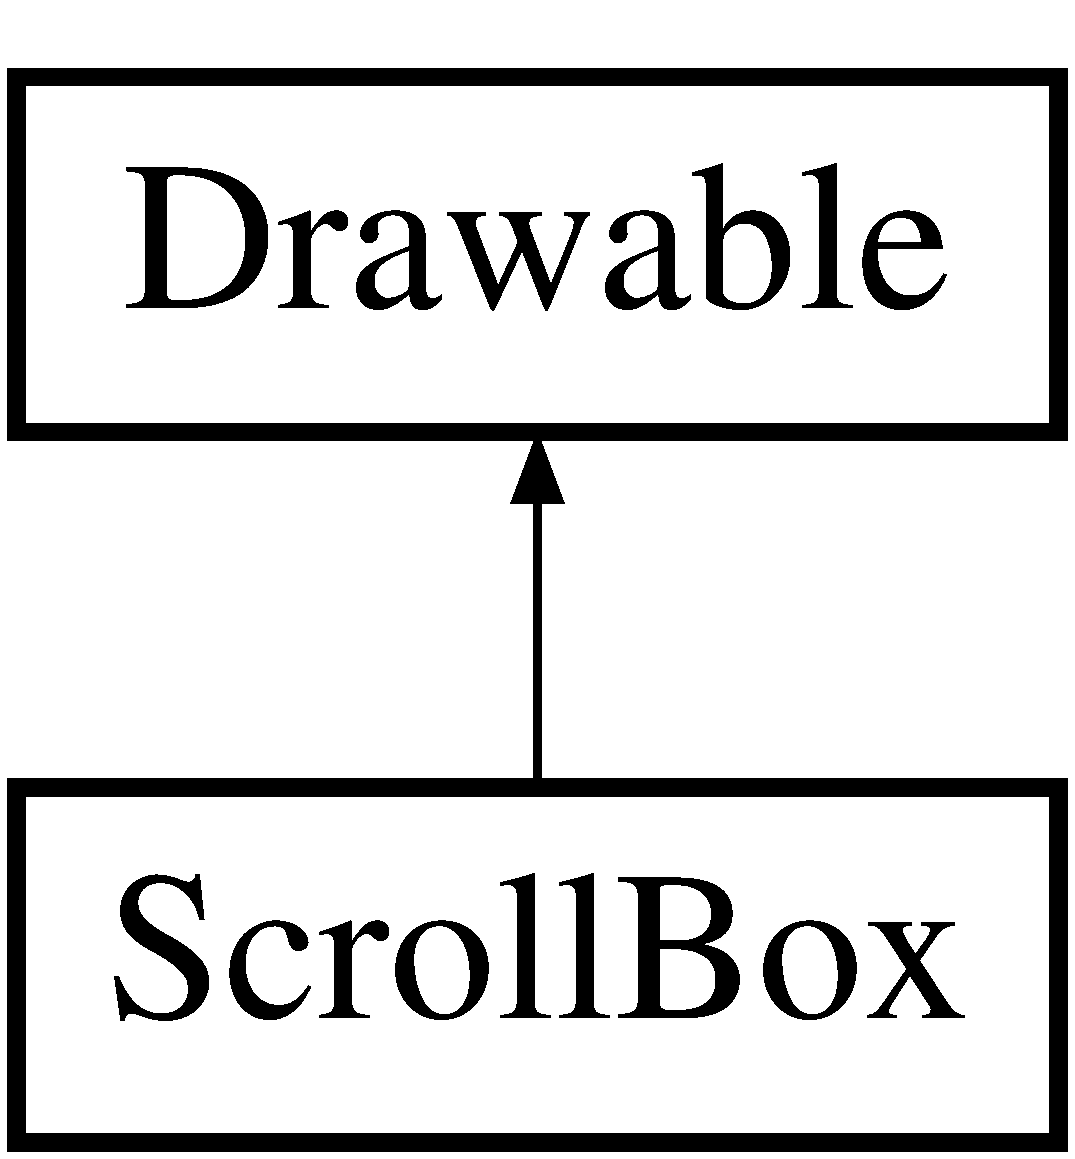
\includegraphics[height=2.000000cm]{class_scroll_box}
\end{center}
\end{figure}
\subsection*{Public Member Functions}
\begin{DoxyCompactItemize}
\item 
\mbox{\Hypertarget{class_scroll_box_a94c60fde856433108c6548f0892ef253}\label{class_scroll_box_a94c60fde856433108c6548f0892ef253}} 
{\bfseries Scroll\+Box} (sf\+::\+Vector2f p\+\_\+\+Pos, sf\+::\+Vector2f p\+\_\+\+Size, sf\+::\+Vector2f p\+\_\+\+Container\+Size, bool p\+\_\+\+Has\+Verti\+Bar, bool p\+\_\+\+Has\+Hori\+Bar)
\item 
\mbox{\Hypertarget{class_scroll_box_a9e2d78a8b045d678e67bb026888a1012}\label{class_scroll_box_a9e2d78a8b045d678e67bb026888a1012}} 
void {\bfseries draw} (sf\+::\+Render\+Target \&target, sf\+::\+Render\+States states) const
\end{DoxyCompactItemize}


The documentation for this class was generated from the following file\+:\begin{DoxyCompactItemize}
\item 
D\+:/\+Sam/\+D\+M\+U/\+Year 3/\+I\+M\+A\+T3451 -\/ Final/\+Animation project repo/\+Animation Tool/\+Animation Project/include/Scroll\+Box.\+h\end{DoxyCompactItemize}

\hypertarget{class_s_f_m_l_input_handler}{}\section{S\+F\+M\+L\+Input\+Handler Class Reference}
\label{class_s_f_m_l_input_handler}\index{S\+F\+M\+L\+Input\+Handler@{S\+F\+M\+L\+Input\+Handler}}


Class that manages S\+F\+ML\textquotesingle{}s input events and notifies thier corresponding signals.  




{\ttfamily \#include $<$Input\+Handler.\+h$>$}

\subsection*{Public Member Functions}
\begin{DoxyCompactItemize}
\item 
\mbox{\Hypertarget{class_s_f_m_l_input_handler_a9e66d308027154e6716957e35b5ec2eb}\label{class_s_f_m_l_input_handler_a9e66d308027154e6716957e35b5ec2eb}} 
\hyperlink{class_s_f_m_l_input_handler_a9e66d308027154e6716957e35b5ec2eb}{S\+F\+M\+L\+Input\+Handler} ()
\begin{DoxyCompactList}\small\item\em Constructor that registers all the signals with the event handler. \end{DoxyCompactList}\item 
\mbox{\Hypertarget{class_s_f_m_l_input_handler_ae57aa5ce6009abe49a0dd12f3b27e5fd}\label{class_s_f_m_l_input_handler_ae57aa5ce6009abe49a0dd12f3b27e5fd}} 
void \hyperlink{class_s_f_m_l_input_handler_ae57aa5ce6009abe49a0dd12f3b27e5fd}{Handle\+Inputs} (sf\+::\+Render\+Window \&p\+\_\+\+Window, sf\+::\+View \&p\+\_\+\+View)
\begin{DoxyCompactList}\small\item\em Handle inputs function (called in the main loop) \end{DoxyCompactList}\end{DoxyCompactItemize}


\subsection{Detailed Description}
Class that manages S\+F\+ML\textquotesingle{}s input events and notifies thier corresponding signals. 

The documentation for this class was generated from the following file\+:\begin{DoxyCompactItemize}
\item 
D\+:/\+Sam/\+D\+M\+U/\+Year 3/\+I\+M\+A\+T3451 -\/ Final/\+Animation project repo/\+Animation Tool/\+Animation Project/include/Input\+Handler.\+h\end{DoxyCompactItemize}

\hypertarget{struct_shape_key_frames}{}\section{Shape\+Key\+Frames Struct Reference}
\label{struct_shape_key_frames}\index{Shape\+Key\+Frames@{Shape\+Key\+Frames}}


Struct that holds the ID and corresponding keyframes.  




{\ttfamily \#include $<$Anim\+Structs.\+h$>$}

\subsection*{Public Attributes}
\begin{DoxyCompactItemize}
\item 
\mbox{\Hypertarget{struct_shape_key_frames_a8abd28a14574b2aa45bd2b291c2cadf9}\label{struct_shape_key_frames_a8abd28a14574b2aa45bd2b291c2cadf9}} 
unsigned int {\bfseries m\+\_\+\+ID}
\item 
\mbox{\Hypertarget{struct_shape_key_frames_a651f83d823261af06d50622f9a010b17}\label{struct_shape_key_frames_a651f83d823261af06d50622f9a010b17}} 
flat\+\_\+set$<$ \hyperlink{struct_key_frame}{Key\+Frame}, \hyperlink{struct_compare_frame}{Compare\+Frame} $>$ {\bfseries m\+\_\+\+Key\+Frames2}
\end{DoxyCompactItemize}


\subsection{Detailed Description}
Struct that holds the ID and corresponding keyframes. 

The documentation for this struct was generated from the following file\+:\begin{DoxyCompactItemize}
\item 
D\+:/\+Sam/\+D\+M\+U/\+Year 3/\+I\+M\+A\+T3451 -\/ Final/\+Animation project repo/\+Animation Tool/\+Animation Project/include/Anim\+Structs.\+h\end{DoxyCompactItemize}

\hypertarget{class_shapes}{}\section{Shapes Class Reference}
\label{class_shapes}\index{Shapes@{Shapes}}


container class that handles the creation and getting of objects via I\+Ds  




{\ttfamily \#include $<$Shapes.\+h$>$}

Inheritance diagram for Shapes\+:\begin{figure}[H]
\begin{center}
\leavevmode
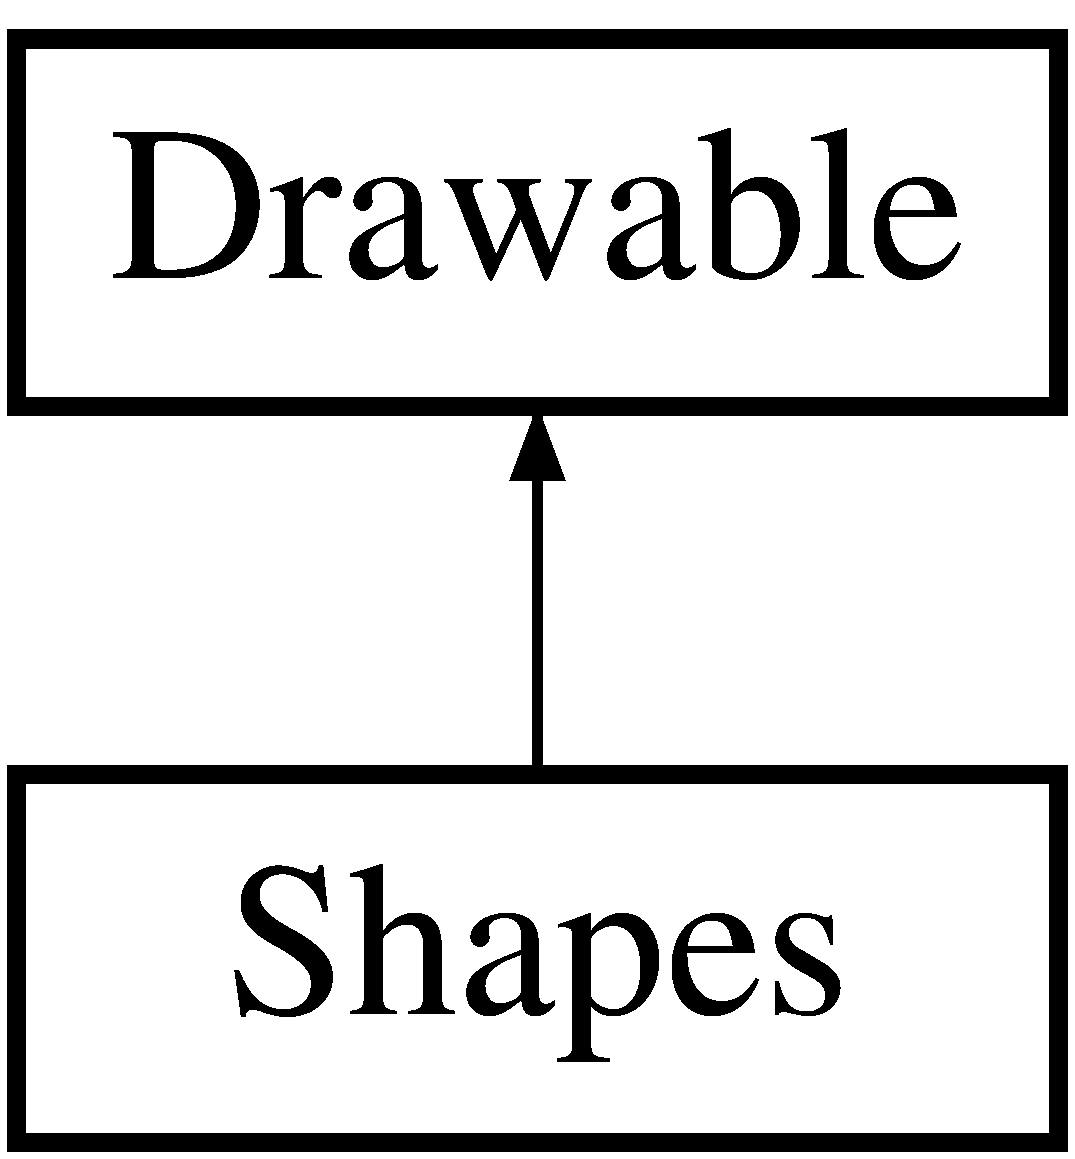
\includegraphics[height=2.000000cm]{class_shapes}
\end{center}
\end{figure}
\subsection*{Public Member Functions}
\begin{DoxyCompactItemize}
\item 
\mbox{\Hypertarget{class_shapes_a507aab492a4840275d9cc6dea090d880}\label{class_shapes_a507aab492a4840275d9cc6dea090d880}} 
std\+::pair$<$ unsigned int, \hyperlink{class_object}{Object} $\ast$ $>$ \hyperlink{class_shapes_a507aab492a4840275d9cc6dea090d880}{New\+Shape} (\hyperlink{class_object}{Object} p\+\_\+\+New\+Object)
\begin{DoxyCompactList}\small\item\em Adds a copy of a shape to the shape map and returns its ID and pointer. \end{DoxyCompactList}\item 
\mbox{\Hypertarget{class_shapes_a95aba282963cca12a01ee17066af9297}\label{class_shapes_a95aba282963cca12a01ee17066af9297}} 
\hyperlink{class_object}{Object} \& \hyperlink{class_shapes_a95aba282963cca12a01ee17066af9297}{Find\+Shape} (unsigned int p\+\_\+\+ID)
\begin{DoxyCompactList}\small\item\em Locates and returns a reference to a shape with ID. \end{DoxyCompactList}\item 
\mbox{\Hypertarget{class_shapes_a8651d6e746556b68623156dcce5202bc}\label{class_shapes_a8651d6e746556b68623156dcce5202bc}} 
std\+::vector$<$ \hyperlink{class_object}{Object} $\ast$ $>$ \hyperlink{class_shapes_a8651d6e746556b68623156dcce5202bc}{Get\+Objects} ()
\begin{DoxyCompactList}\small\item\em Returns a vector with pointers to all the current objects in the map. \end{DoxyCompactList}\item 
\mbox{\Hypertarget{class_shapes_ab1d661641f51d136fd840367562580ef}\label{class_shapes_ab1d661641f51d136fd840367562580ef}} 
std\+::map$<$ unsigned int, \hyperlink{class_object_data}{Object\+Data} $>$ \hyperlink{class_shapes_ab1d661641f51d136fd840367562580ef}{Get\+I\+D\+And\+Datas} ()
\begin{DoxyCompactList}\small\item\em Returns a map containing all the I\+Ds and object data of shapes currently in the shapes map. \end{DoxyCompactList}\item 
\mbox{\Hypertarget{class_shapes_a0de59bfbb215384f9027301817bcd4a1}\label{class_shapes_a0de59bfbb215384f9027301817bcd4a1}} 
std\+::map$<$ unsigned int, \hyperlink{class_object}{Object} $\ast$ $>$ \hyperlink{class_shapes_a0de59bfbb215384f9027301817bcd4a1}{Get\+I\+D\+And\+Objects} ()
\begin{DoxyCompactList}\small\item\em Returns a map of I\+Ds and object pointers. \end{DoxyCompactList}\item 
\mbox{\Hypertarget{class_shapes_a7dbae8132686e181679f4a543b0dc128}\label{class_shapes_a7dbae8132686e181679f4a543b0dc128}} 
void \hyperlink{class_shapes_a7dbae8132686e181679f4a543b0dc128}{Delete\+Shape} (unsigned int p\+\_\+\+ID)
\begin{DoxyCompactList}\small\item\em Deletes an object with associated ID. \end{DoxyCompactList}\item 
\mbox{\Hypertarget{class_shapes_a4cb9b0b2e974c63e3182103626b582a4}\label{class_shapes_a4cb9b0b2e974c63e3182103626b582a4}} 
unsigned int \hyperlink{class_shapes_a4cb9b0b2e974c63e3182103626b582a4}{Get\+Size} ()
\begin{DoxyCompactList}\small\item\em returns the size of the shapes\textquotesingle{} map \end{DoxyCompactList}\item 
\mbox{\Hypertarget{class_shapes_aab0b2aa58534e707e13f8651f5a6e55d}\label{class_shapes_aab0b2aa58534e707e13f8651f5a6e55d}} 
void \hyperlink{class_shapes_aab0b2aa58534e707e13f8651f5a6e55d}{Update\+Shapes} ()
\begin{DoxyCompactList}\small\item\em calls all the shapes update methods \end{DoxyCompactList}\item 
\mbox{\Hypertarget{class_shapes_a5d0ed4de4f10f3a81f2eff482550c448}\label{class_shapes_a5d0ed4de4f10f3a81f2eff482550c448}} 
void \hyperlink{class_shapes_a5d0ed4de4f10f3a81f2eff482550c448}{draw} (sf\+::\+Render\+Target \&target, sf\+::\+Render\+States states) const
\begin{DoxyCompactList}\small\item\em Draws the shapes. \end{DoxyCompactList}\end{DoxyCompactItemize}
\subsection*{Public Attributes}
\begin{DoxyCompactItemize}
\item 
\mbox{\Hypertarget{class_shapes_aa818577f33ff41432500e96cfb07d1f9}\label{class_shapes_aa818577f33ff41432500e96cfb07d1f9}} 
\hyperlink{class_signal}{Signal}$<$ unsigned int $>$ \hyperlink{class_shapes_aa818577f33ff41432500e96cfb07d1f9}{On\+Created}
\begin{DoxyCompactList}\small\item\em \hyperlink{class_signal}{Signal} for creation of shapes. \end{DoxyCompactList}\end{DoxyCompactItemize}


\subsection{Detailed Description}
container class that handles the creation and getting of objects via I\+Ds 

The documentation for this class was generated from the following files\+:\begin{DoxyCompactItemize}
\item 
D\+:/\+Sam/\+D\+M\+U/\+Year 3/\+I\+M\+A\+T3451 -\/ Final/\+Animation project repo/\+Animation Tool/\+Animation Project/include/Shapes.\+h\item 
D\+:/\+Sam/\+D\+M\+U/\+Year 3/\+I\+M\+A\+T3451 -\/ Final/\+Animation project repo/\+Animation Tool/\+Animation Project/include/Shapes.\+cpp\end{DoxyCompactItemize}

\hypertarget{struct_shape_slot}{}\section{Shape\+Slot Struct Reference}
\label{struct_shape_slot}\index{Shape\+Slot@{Shape\+Slot}}


Struct that holds data for shape slots and their corrisponding frame slots.  




{\ttfamily \#include $<$Time\+Line.\+h$>$}

\subsection*{Public Attributes}
\begin{DoxyCompactItemize}
\item 
\mbox{\Hypertarget{struct_shape_slot_a523bedf57f5eaae9a7fb5de2dd301949}\label{struct_shape_slot_a523bedf57f5eaae9a7fb5de2dd301949}} 
bool {\bfseries m\+\_\+\+Active} = false
\item 
\mbox{\Hypertarget{struct_shape_slot_a86672abb1093de577b94122c3727363d}\label{struct_shape_slot_a86672abb1093de577b94122c3727363d}} 
sf\+::\+Rectangle\+Shape {\bfseries m\+\_\+\+Rect}
\item 
\mbox{\Hypertarget{struct_shape_slot_ac44e81e4ec1486a4a559cc6260079f7c}\label{struct_shape_slot_ac44e81e4ec1486a4a559cc6260079f7c}} 
unsigned int {\bfseries m\+\_\+\+ID}
\item 
\mbox{\Hypertarget{struct_shape_slot_ad59dcd642205553eb786a5fd97e7fb98}\label{struct_shape_slot_ad59dcd642205553eb786a5fd97e7fb98}} 
std\+::vector$<$ \hyperlink{struct_frame_slot}{Frame\+Slot} $>$ {\bfseries m\+\_\+\+Frame\+Slots}
\item 
\mbox{\Hypertarget{struct_shape_slot_aad2e2b96f2145ac1fd16ea2582c060eb}\label{struct_shape_slot_aad2e2b96f2145ac1fd16ea2582c060eb}} 
sf\+::\+Text {\bfseries m\+\_\+\+Text}
\end{DoxyCompactItemize}


\subsection{Detailed Description}
Struct that holds data for shape slots and their corrisponding frame slots. 

The documentation for this struct was generated from the following file\+:\begin{DoxyCompactItemize}
\item 
D\+:/\+Sam/\+D\+M\+U/\+Year 3/\+I\+M\+A\+T3451 -\/ Final/\+Animation project repo/\+Animation Tool/\+Animation Project/include/Time\+Line.\+h\end{DoxyCompactItemize}

\hypertarget{class_shape_tool}{}\section{Shape\+Tool Class Reference}
\label{class_shape_tool}\index{Shape\+Tool@{Shape\+Tool}}


Handles the drawing and creation of a shape.  




{\ttfamily \#include $<$Shape\+Tool.\+h$>$}

Inheritance diagram for Shape\+Tool\+:\begin{figure}[H]
\begin{center}
\leavevmode
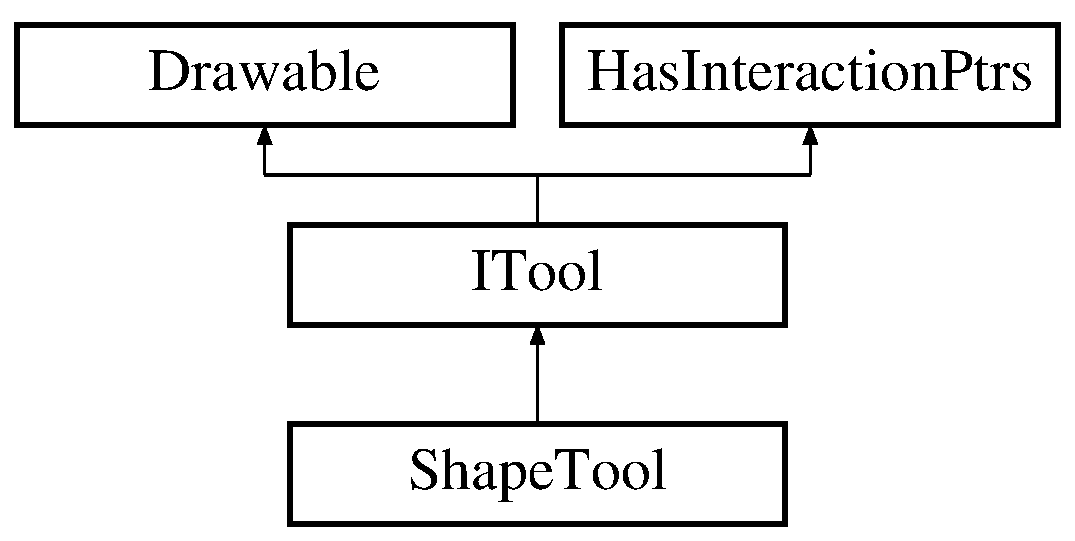
\includegraphics[height=3.000000cm]{class_shape_tool}
\end{center}
\end{figure}
\subsection*{Public Member Functions}
\begin{DoxyCompactItemize}
\item 
\mbox{\Hypertarget{class_shape_tool_a2d31f92499677b36c002b26af0bcd147}\label{class_shape_tool_a2d31f92499677b36c002b26af0bcd147}} 
\hyperlink{class_shape_tool_a2d31f92499677b36c002b26af0bcd147}{Shape\+Tool} (\hyperlink{struct_interaction_ptrs}{Interaction\+Ptrs} $\ast$p\+\_\+p\+SP)
\begin{DoxyCompactList}\small\item\em Constructor that takes the interaction\+Ptrs that contain useful classes for the creation of new shapes. \end{DoxyCompactList}\item 
\mbox{\Hypertarget{class_shape_tool_a098c92b3a500ab0626c73e078dbdbddc}\label{class_shape_tool_a098c92b3a500ab0626c73e078dbdbddc}} 
void \hyperlink{class_shape_tool_a098c92b3a500ab0626c73e078dbdbddc}{Update} (float p\+\_\+\+Delta\+Time) override
\begin{DoxyCompactList}\small\item\em update method used to visually update the shape benig drawn \end{DoxyCompactList}\item 
\mbox{\Hypertarget{class_shape_tool_a96dbd9eb07a88d3855d5f2fbd71f5474}\label{class_shape_tool_a96dbd9eb07a88d3855d5f2fbd71f5474}} 
void \hyperlink{class_shape_tool_a96dbd9eb07a88d3855d5f2fbd71f5474}{On\+Mouse\+Click} (sf\+::\+Mouse\+::\+Button p\+\_\+\+Button, bool p\+\_\+b\+State) override
\begin{DoxyCompactList}\small\item\em callback that is called on the mouse being clicked \end{DoxyCompactList}\end{DoxyCompactItemize}
\subsection*{Additional Inherited Members}


\subsection{Detailed Description}
Handles the drawing and creation of a shape. 

The documentation for this class was generated from the following file\+:\begin{DoxyCompactItemize}
\item 
D\+:/\+Sam/\+D\+M\+U/\+Year 3/\+I\+M\+A\+T3451 -\/ Final/\+Animation project repo/\+Animation Tool/\+Animation Project/include/Shape\+Tool.\+h\end{DoxyCompactItemize}

\hypertarget{class_signal}{}\section{Signal$<$ Args $>$ Class Template Reference}
\label{class_signal}\index{Signal$<$ Args $>$@{Signal$<$ Args $>$}}


Handles the connections of call back functions.  




{\ttfamily \#include $<$Signal.\+h$>$}

\subsection*{Public Member Functions}
\begin{DoxyCompactItemize}
\item 
\mbox{\Hypertarget{class_signal_a3437b8fd65f60a38d45d4d92349dd544}\label{class_signal_a3437b8fd65f60a38d45d4d92349dd544}} 
\hyperlink{class_signal_a3437b8fd65f60a38d45d4d92349dd544}{Signal} ()
\begin{DoxyCompactList}\small\item\em Constructor sets the ID to 0. \end{DoxyCompactList}\item 
\mbox{\Hypertarget{class_signal_a249b93a84b73e8bda0373f6595e6724f}\label{class_signal_a249b93a84b73e8bda0373f6595e6724f}} 
\hyperlink{class_signal_a249b93a84b73e8bda0373f6595e6724f}{Signal} (\hyperlink{class_signal}{Signal} const \&p\+\_\+\+Signal)
\begin{DoxyCompactList}\small\item\em Copy constructor makes sure the ID is still 0. \end{DoxyCompactList}\item 
\mbox{\Hypertarget{class_signal_a3ddf10ab607a60af919faa9494836e9e}\label{class_signal_a3ddf10ab607a60af919faa9494836e9e}} 
int \hyperlink{class_signal_a3ddf10ab607a60af919faa9494836e9e}{Connect} (F\+U\+N\+C\+\_\+\+P\+TR const \&p\+\_\+\+Listener) const
\begin{DoxyCompactList}\small\item\em Connection method takes a std\+::functional function pointer and emplaces it to the map. \end{DoxyCompactList}\item 
\mbox{\Hypertarget{class_signal_a7fe765fc1c513307fd7ae28f0f907f0d}\label{class_signal_a7fe765fc1c513307fd7ae28f0f907f0d}} 
void \hyperlink{class_signal_a7fe765fc1c513307fd7ae28f0f907f0d}{Disconnect} (int p\+\_\+\+ID) const
\begin{DoxyCompactList}\small\item\em Disconnect method erases a callback with ID p\+\_\+\+ID. \end{DoxyCompactList}\item 
\mbox{\Hypertarget{class_signal_a84a53c35c242b67e1e6fbb3d1545eed8}\label{class_signal_a84a53c35c242b67e1e6fbb3d1545eed8}} 
void \hyperlink{class_signal_a84a53c35c242b67e1e6fbb3d1545eed8}{Disconect\+All} () const
\begin{DoxyCompactList}\small\item\em Disconnect all callback functions. \end{DoxyCompactList}\item 
\mbox{\Hypertarget{class_signal_a3e5a119b3f1946bdd722518039d4f36d}\label{class_signal_a3e5a119b3f1946bdd722518039d4f36d}} 
void \hyperlink{class_signal_a3e5a119b3f1946bdd722518039d4f36d}{Notify} (Args... p\+\_\+\+Args)
\begin{DoxyCompactList}\small\item\em Calls and passes the given arguments to all callback functions. \end{DoxyCompactList}\item 
\mbox{\Hypertarget{class_signal_ae06f307f87638c3d59a8453bf9031fec}\label{class_signal_ae06f307f87638c3d59a8453bf9031fec}} 
\hyperlink{class_signal}{Signal} \& \hyperlink{class_signal_ae06f307f87638c3d59a8453bf9031fec}{operator=} (\hyperlink{class_signal}{Signal} const \&p\+\_\+\+Signal)
\begin{DoxyCompactList}\small\item\em Overloaded assignment operator disconnects all callbacks. \end{DoxyCompactList}\end{DoxyCompactItemize}


\subsection{Detailed Description}
\subsubsection*{template$<$typename... Args$>$\newline
class Signal$<$ Args $>$}

Handles the connections of call back functions. 

The documentation for this class was generated from the following file\+:\begin{DoxyCompactItemize}
\item 
D\+:/\+Sam/\+D\+M\+U/\+Year 3/\+I\+M\+A\+T3451 -\/ Final/\+Animation project repo/\+Animation Tool/\+Animation Project/include/Signal.\+h\end{DoxyCompactItemize}

\hypertarget{class_slider}{}\section{Slider Class Reference}
\label{class_slider}\index{Slider@{Slider}}


Used to create a very simple slider.  




{\ttfamily \#include $<$Slider.\+h$>$}

Inheritance diagram for Slider\+:\begin{figure}[H]
\begin{center}
\leavevmode
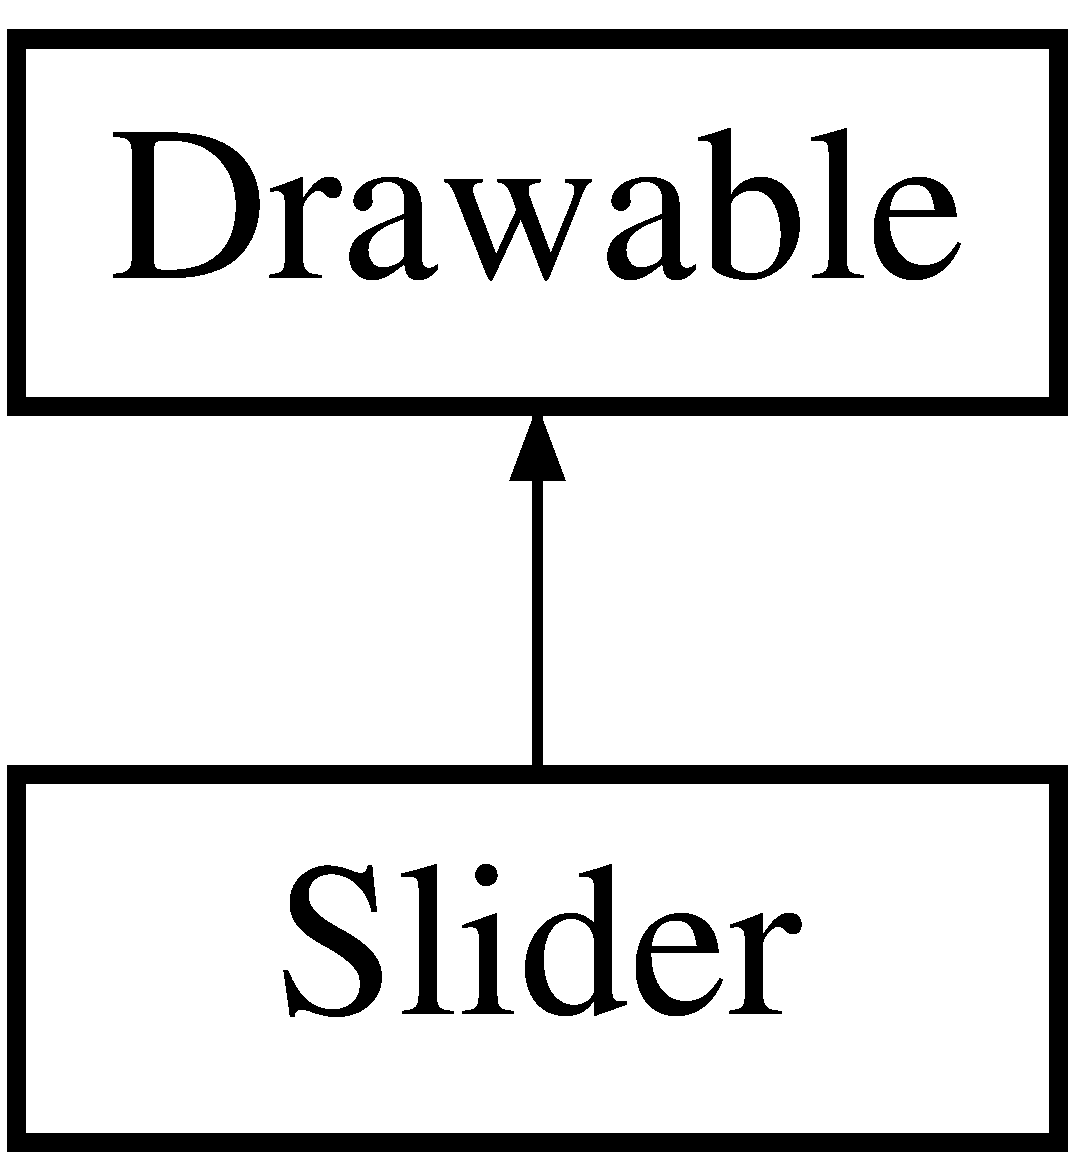
\includegraphics[height=2.000000cm]{class_slider}
\end{center}
\end{figure}
\subsection*{Public Member Functions}
\begin{DoxyCompactItemize}
\item 
\mbox{\Hypertarget{class_slider_a535033fada8e25ef7291d2a52e6e437b}\label{class_slider_a535033fada8e25ef7291d2a52e6e437b}} 
\hyperlink{class_slider_a535033fada8e25ef7291d2a52e6e437b}{Slider} ()
\begin{DoxyCompactList}\small\item\em constructor \end{DoxyCompactList}\item 
\mbox{\Hypertarget{class_slider_a94344aa7908201fb6caa76d39f8bde88}\label{class_slider_a94344aa7908201fb6caa76d39f8bde88}} 
\hyperlink{class_slider_a94344aa7908201fb6caa76d39f8bde88}{Slider} (sf\+::\+Vector2f p\+\_\+\+Pos, float p\+\_\+\+Length)
\begin{DoxyCompactList}\small\item\em constructor that takes position and length \end{DoxyCompactList}\item 
\mbox{\Hypertarget{class_slider_a0573daabd36577e4ed2364352e375c22}\label{class_slider_a0573daabd36577e4ed2364352e375c22}} 
void \hyperlink{class_slider_a0573daabd36577e4ed2364352e375c22}{Handle\+Mouse\+Input} (sf\+::\+Mouse\+::\+Button p\+\_\+\+Button, bool p\+\_\+\+State)
\begin{DoxyCompactList}\small\item\em Callback that handles the mouse button events. \end{DoxyCompactList}\item 
\mbox{\Hypertarget{class_slider_aeb1da2f98fcc1ccdd71703b7e23181c7}\label{class_slider_aeb1da2f98fcc1ccdd71703b7e23181c7}} 
void \hyperlink{class_slider_aeb1da2f98fcc1ccdd71703b7e23181c7}{Handle\+Mouse\+Move} (sf\+::\+Vector2i l\+\_\+\+Mouse\+Pos)
\begin{DoxyCompactList}\small\item\em Callback that handles the mouse move events. \end{DoxyCompactList}\item 
\mbox{\Hypertarget{class_slider_a1e57a096aedaaa37030a85aeb4e7302f}\label{class_slider_a1e57a096aedaaa37030a85aeb4e7302f}} 
void \hyperlink{class_slider_a1e57a096aedaaa37030a85aeb4e7302f}{Set\+Length} (float p\+\_\+\+Length)
\begin{DoxyCompactList}\small\item\em Length of the slider setter. \end{DoxyCompactList}\item 
\mbox{\Hypertarget{class_slider_a1d3ab32779278798ccb2410648282036}\label{class_slider_a1d3ab32779278798ccb2410648282036}} 
void \hyperlink{class_slider_a1d3ab32779278798ccb2410648282036}{set\+Position} (sf\+::\+Vector2f p\+\_\+\+Pos)
\begin{DoxyCompactList}\small\item\em Position setter. \end{DoxyCompactList}\item 
\mbox{\Hypertarget{class_slider_ab49809e3c428a3c3783efd49a148c6f7}\label{class_slider_ab49809e3c428a3c3783efd49a148c6f7}} 
float \hyperlink{class_slider_ab49809e3c428a3c3783efd49a148c6f7}{get\+Percent} ()
\begin{DoxyCompactList}\small\item\em Percentage that the bar has progress getter. \end{DoxyCompactList}\item 
\mbox{\Hypertarget{class_slider_aab959e9d386bd5e6f7953ad11cbd49f6}\label{class_slider_aab959e9d386bd5e6f7953ad11cbd49f6}} 
void \hyperlink{class_slider_aab959e9d386bd5e6f7953ad11cbd49f6}{draw} (sf\+::\+Render\+Target \&target, sf\+::\+Render\+States states) const
\begin{DoxyCompactList}\small\item\em Draw method draws the UI. \end{DoxyCompactList}\end{DoxyCompactItemize}


\subsection{Detailed Description}
Used to create a very simple slider. 

The documentation for this class was generated from the following file\+:\begin{DoxyCompactItemize}
\item 
D\+:/\+Sam/\+D\+M\+U/\+Year 3/\+I\+M\+A\+T3451 -\/ Final/\+Animation project repo/\+Animation Tool/\+Animation Project/include/Slider.\+h\end{DoxyCompactItemize}

\hypertarget{class_q_1_1_time}{}\section{Q\+:\+:Time Class Reference}
\label{class_q_1_1_time}\index{Q\+::\+Time@{Q\+::\+Time}}
Inheritance diagram for Q\+:\+:Time\+:\begin{figure}[H]
\begin{center}
\leavevmode
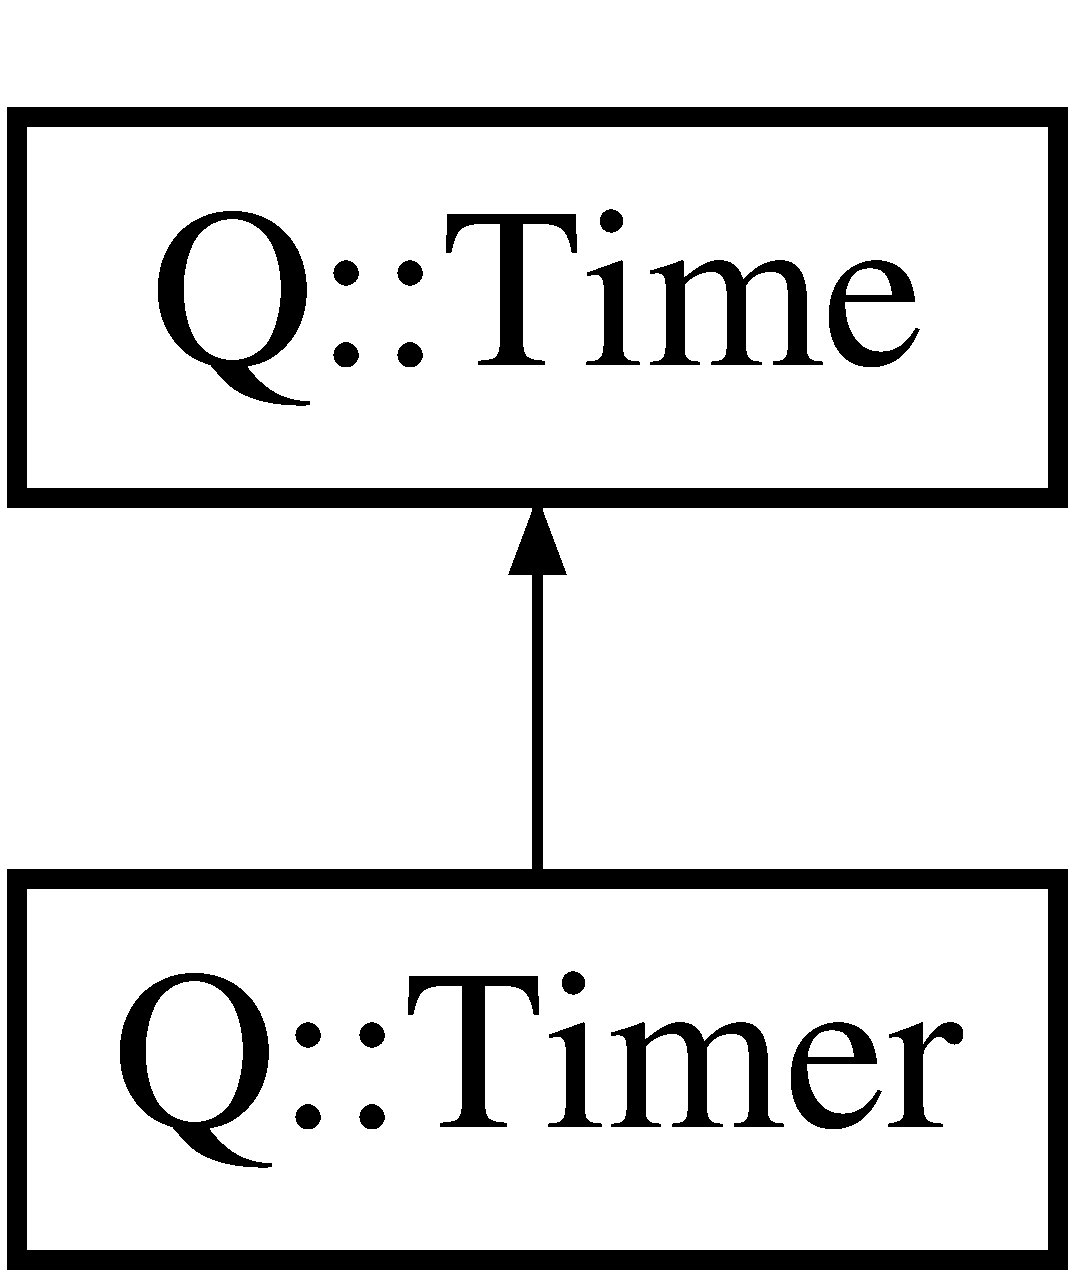
\includegraphics[height=2.000000cm]{class_q_1_1_time}
\end{center}
\end{figure}
\subsection*{Public Member Functions}
\begin{DoxyCompactItemize}
\item 
\mbox{\Hypertarget{class_q_1_1_time_ac72848b1ffb63c184cd312738b5cc2ed}\label{class_q_1_1_time_ac72848b1ffb63c184cd312738b5cc2ed}} 
{\bfseries Time} (unsigned int p\+\_\+\+Hours, unsigned int p\+\_\+\+Minutes, double p\+\_\+\+Seconds)
\item 
\mbox{\Hypertarget{class_q_1_1_time_a2bcb2fc8b2101517aa5b2409b86963a6}\label{class_q_1_1_time_a2bcb2fc8b2101517aa5b2409b86963a6}} 
double {\bfseries Get\+Seconds} ()
\item 
\mbox{\Hypertarget{class_q_1_1_time_adade232803ba1570d53182c997829d1c}\label{class_q_1_1_time_adade232803ba1570d53182c997829d1c}} 
int {\bfseries Get\+Minutes} ()
\item 
\mbox{\Hypertarget{class_q_1_1_time_a9000bbd6010a5c20f5c9d0f1bca7bbf8}\label{class_q_1_1_time_a9000bbd6010a5c20f5c9d0f1bca7bbf8}} 
int {\bfseries Get\+Hours} ()
\item 
\mbox{\Hypertarget{class_q_1_1_time_a075ce41503d52f7939616eca06cbcfbf}\label{class_q_1_1_time_a075ce41503d52f7939616eca06cbcfbf}} 
void {\bfseries Set\+Seconds} (double p\+\_\+\+Seconds)
\item 
\mbox{\Hypertarget{class_q_1_1_time_a5e95992d560c4dacbde1b97135e43104}\label{class_q_1_1_time_a5e95992d560c4dacbde1b97135e43104}} 
void {\bfseries Set\+Minutes} (unsigned int p\+\_\+\+Minutes)
\item 
\mbox{\Hypertarget{class_q_1_1_time_a70ef5e519c1ef050a4d1f37a192177c0}\label{class_q_1_1_time_a70ef5e519c1ef050a4d1f37a192177c0}} 
void {\bfseries Set\+Hours} (unsigned int p\+\_\+\+Hours)
\end{DoxyCompactItemize}
\subsection*{Protected Attributes}
\begin{DoxyCompactItemize}
\item 
\mbox{\Hypertarget{class_q_1_1_time_a5656ba36518d75edbfbedb5d8b8d68d7}\label{class_q_1_1_time_a5656ba36518d75edbfbedb5d8b8d68d7}} 
double {\bfseries m\+\_\+\+Seconds} = 0
\item 
\mbox{\Hypertarget{class_q_1_1_time_afe9a334e8fcd9970c34dd8c3ee119c89}\label{class_q_1_1_time_afe9a334e8fcd9970c34dd8c3ee119c89}} 
int {\bfseries m\+\_\+\+Minutes} = 0
\item 
\mbox{\Hypertarget{class_q_1_1_time_a9628290ab6284dc03258744faccabe9d}\label{class_q_1_1_time_a9628290ab6284dc03258744faccabe9d}} 
int {\bfseries m\+\_\+\+Hours} = 0
\end{DoxyCompactItemize}


The documentation for this class was generated from the following files\+:\begin{DoxyCompactItemize}
\item 
D\+:/\+Sam/\+D\+M\+U/\+Year 3/\+I\+M\+A\+T3451 -\/ Final/\+Animation project repo/\+Animation Tool/\+Animation Project/include/Timer.\+h\item 
D\+:/\+Sam/\+D\+M\+U/\+Year 3/\+I\+M\+A\+T3451 -\/ Final/\+Animation project repo/\+Animation Tool/\+Animation Project/include/Timer.\+cpp\end{DoxyCompactItemize}

\hypertarget{class_time_line}{}\section{Time\+Line Class Reference}
\label{class_time_line}\index{Time\+Line@{Time\+Line}}


Creates and manages a user interface to deal with \char`\"{}\+Shape\+Key\+Frame\char`\"{} data.  




{\ttfamily \#include $<$Time\+Line.\+h$>$}

Inheritance diagram for Time\+Line\+:\begin{figure}[H]
\begin{center}
\leavevmode
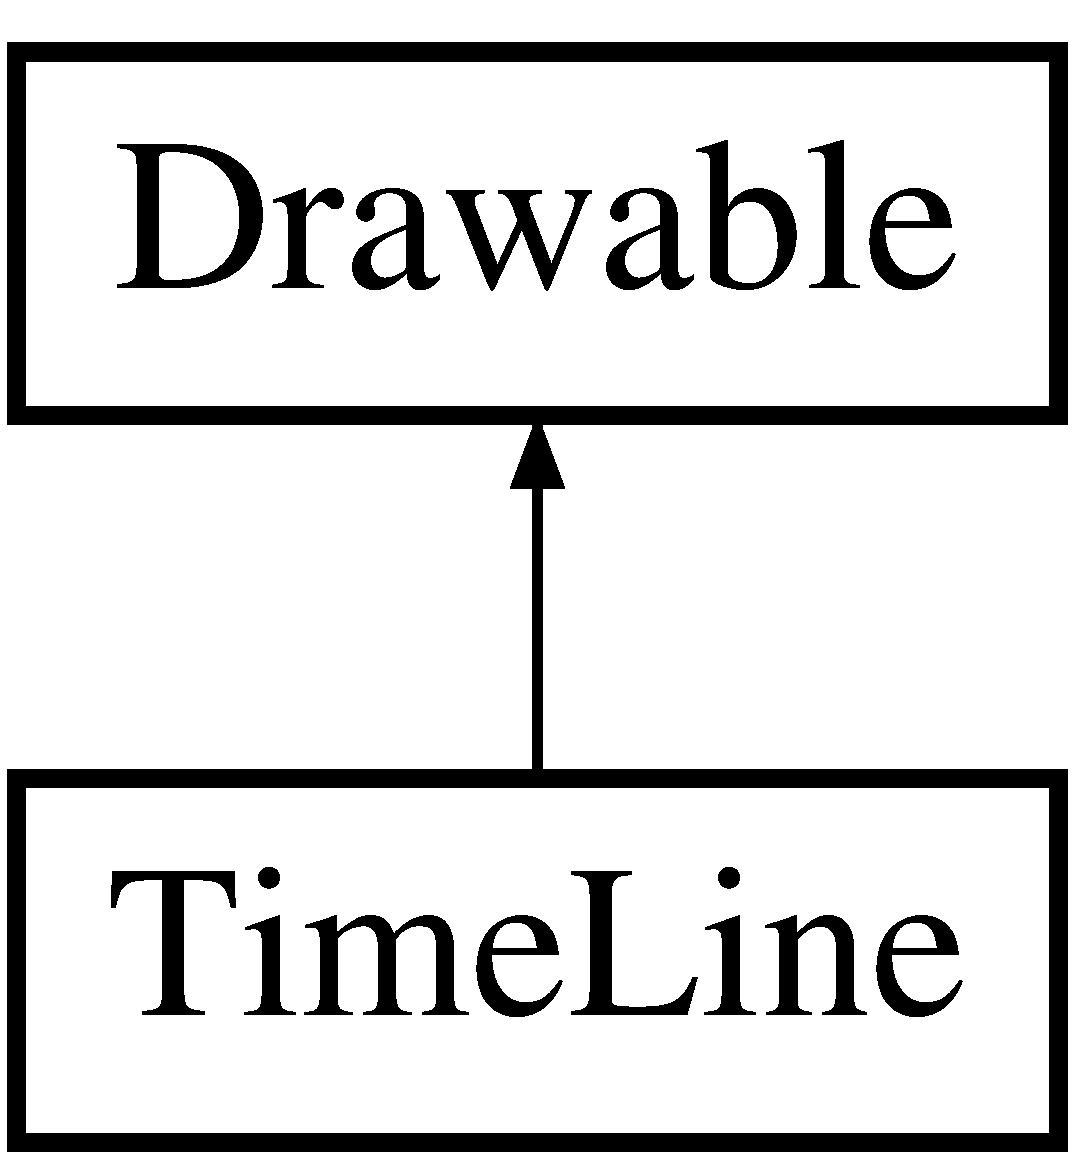
\includegraphics[height=2.000000cm]{class_time_line}
\end{center}
\end{figure}
\subsection*{Public Member Functions}
\begin{DoxyCompactItemize}
\item 
\mbox{\Hypertarget{class_time_line_a48cda2f285f06a06211724178d01383d}\label{class_time_line_a48cda2f285f06a06211724178d01383d}} 
\hyperlink{class_time_line_a48cda2f285f06a06211724178d01383d}{Time\+Line} (sf\+::\+Vector2f p\+\_\+\+Pos, sf\+::\+Vector2f p\+\_\+\+Size, unsigned int p\+\_\+\+Frame\+Rate, unsigned int p\+\_\+\+Total\+Frames)
\begin{DoxyCompactList}\small\item\em Constructor. \end{DoxyCompactList}\item 
\mbox{\Hypertarget{class_time_line_abd8b8a4340ad3dda404a7b48d5b1e0f9}\label{class_time_line_abd8b8a4340ad3dda404a7b48d5b1e0f9}} 
void \hyperlink{class_time_line_abd8b8a4340ad3dda404a7b48d5b1e0f9}{Update} (const flat\+\_\+set$<$ \hyperlink{struct_shape_key_frames}{Shape\+Key\+Frames}, \hyperlink{struct_compare_id}{Compare\+Id} $>$ \&p\+\_\+\+Shapes\+And\+Keys, Frame\+State p\+\_\+\+Frame\+State)
\begin{DoxyCompactList}\small\item\em Update the shape and frame slots with the keyframe data. \end{DoxyCompactList}\item 
\mbox{\Hypertarget{class_time_line_a5792226d36ccba7466e7f2986fd0702a}\label{class_time_line_a5792226d36ccba7466e7f2986fd0702a}} 
void \hyperlink{class_time_line_a5792226d36ccba7466e7f2986fd0702a}{draw} (sf\+::\+Render\+Target \&target, sf\+::\+Render\+States states) const
\begin{DoxyCompactList}\small\item\em draw the the UI \end{DoxyCompactList}\item 
\mbox{\Hypertarget{class_time_line_a280a51390bb34ebe26a434b871f81add}\label{class_time_line_a280a51390bb34ebe26a434b871f81add}} 
void \hyperlink{class_time_line_a280a51390bb34ebe26a434b871f81add}{On\+Mouse\+Click} (bool p\+\_\+\+State)
\begin{DoxyCompactList}\small\item\em callback for mouse click \end{DoxyCompactList}\item 
\mbox{\Hypertarget{class_time_line_a30ecec78f9815577bd56715ba697e7c6}\label{class_time_line_a30ecec78f9815577bd56715ba697e7c6}} 
void \hyperlink{class_time_line_a30ecec78f9815577bd56715ba697e7c6}{On\+Mouse\+Move} (sf\+::\+Vector2i p\+\_\+\+Pos)
\begin{DoxyCompactList}\small\item\em callback for mouse move \end{DoxyCompactList}\end{DoxyCompactItemize}
\subsection*{Public Attributes}
\begin{DoxyCompactItemize}
\item 
\mbox{\Hypertarget{class_time_line_a250b77331838512edd9656bf12169e9d}\label{class_time_line_a250b77331838512edd9656bf12169e9d}} 
\hyperlink{class_signal}{Signal}$<$ unsigned int $>$ \hyperlink{class_time_line_a250b77331838512edd9656bf12169e9d}{Set\+Key\+Frame}
\begin{DoxyCompactList}\small\item\em \hyperlink{class_signal}{Signal} for keyframe being set. \end{DoxyCompactList}\end{DoxyCompactItemize}


\subsection{Detailed Description}
Creates and manages a user interface to deal with \char`\"{}\+Shape\+Key\+Frame\char`\"{} data. 

The documentation for this class was generated from the following file\+:\begin{DoxyCompactItemize}
\item 
D\+:/\+Sam/\+D\+M\+U/\+Year 3/\+I\+M\+A\+T3451 -\/ Final/\+Animation project repo/\+Animation Tool/\+Animation Project/include/Time\+Line.\+h\end{DoxyCompactItemize}

\hypertarget{class_time_line_viewer}{}\section{Time\+Line\+Viewer Class Reference}
\label{class_time_line_viewer}\index{Time\+Line\+Viewer@{Time\+Line\+Viewer}}
Inheritance diagram for Time\+Line\+Viewer\+:\begin{figure}[H]
\begin{center}
\leavevmode
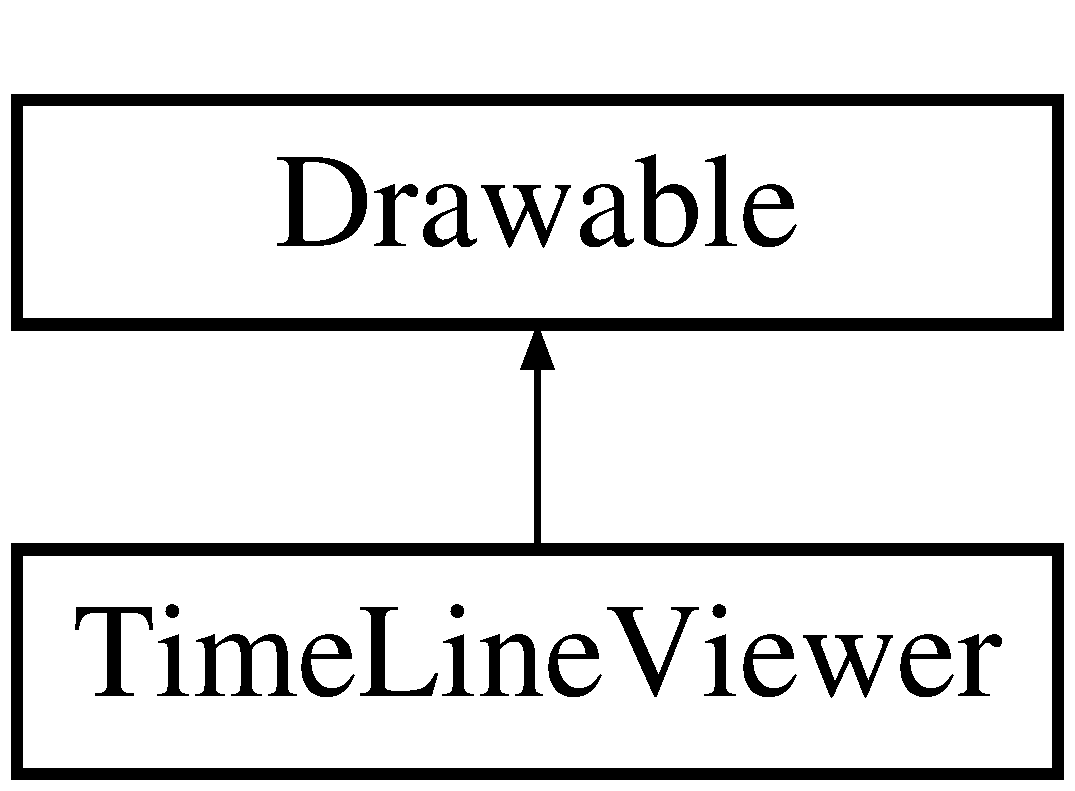
\includegraphics[height=2.000000cm]{class_time_line_viewer}
\end{center}
\end{figure}
\subsection*{Public Member Functions}
\begin{DoxyCompactItemize}
\item 
\mbox{\Hypertarget{class_time_line_viewer_a9a411e81c5399f73d383b9166e113f26}\label{class_time_line_viewer_a9a411e81c5399f73d383b9166e113f26}} 
{\bfseries Time\+Line\+Viewer} (sf\+::\+Vector2f p\+\_\+\+Pos, sf\+::\+Vector2f p\+\_\+\+Size)
\item 
\mbox{\Hypertarget{class_time_line_viewer_a408245f35ad6afe20ab06f0affe95c90}\label{class_time_line_viewer_a408245f35ad6afe20ab06f0affe95c90}} 
void {\bfseries Set\+Total\+Frames} (unsigned int p\+\_\+\+Number\+Of\+Frames)
\item 
\mbox{\Hypertarget{class_time_line_viewer_a99c49e442d49585fcec4f17361a54b02}\label{class_time_line_viewer_a99c49e442d49585fcec4f17361a54b02}} 
void {\bfseries On\+Mouse\+Click} (bool p\+\_\+\+State)
\item 
\mbox{\Hypertarget{class_time_line_viewer_a1dbe935d865141b276abf3202b77c4c2}\label{class_time_line_viewer_a1dbe935d865141b276abf3202b77c4c2}} 
void {\bfseries On\+Mouse\+Move} (sf\+::\+Vector2i p\+\_\+\+Pos)
\item 
\mbox{\Hypertarget{class_time_line_viewer_a3bcb578ec9bdddfe98d9bb367bcc11e8}\label{class_time_line_viewer_a3bcb578ec9bdddfe98d9bb367bcc11e8}} 
void {\bfseries Update} ()
\item 
\mbox{\Hypertarget{class_time_line_viewer_a9d9fbe5a0080fa3207a65cc58c0c5267}\label{class_time_line_viewer_a9d9fbe5a0080fa3207a65cc58c0c5267}} 
void {\bfseries draw} (sf\+::\+Render\+Target \&target, sf\+::\+Render\+States states) const
\end{DoxyCompactItemize}


The documentation for this class was generated from the following file\+:\begin{DoxyCompactItemize}
\item 
D\+:/\+Sam/\+D\+M\+U/\+Year 3/\+I\+M\+A\+T3451 -\/ Final/\+Animation project repo/\+Animation Tool/\+Animation Project/include/Time\+Line\+Viewer.\+h\end{DoxyCompactItemize}

\hypertarget{class_q_1_1_timer}{}\section{Q\+:\+:Timer Class Reference}
\label{class_q_1_1_timer}\index{Q\+::\+Timer@{Q\+::\+Timer}}
Inheritance diagram for Q\+:\+:Timer\+:\begin{figure}[H]
\begin{center}
\leavevmode
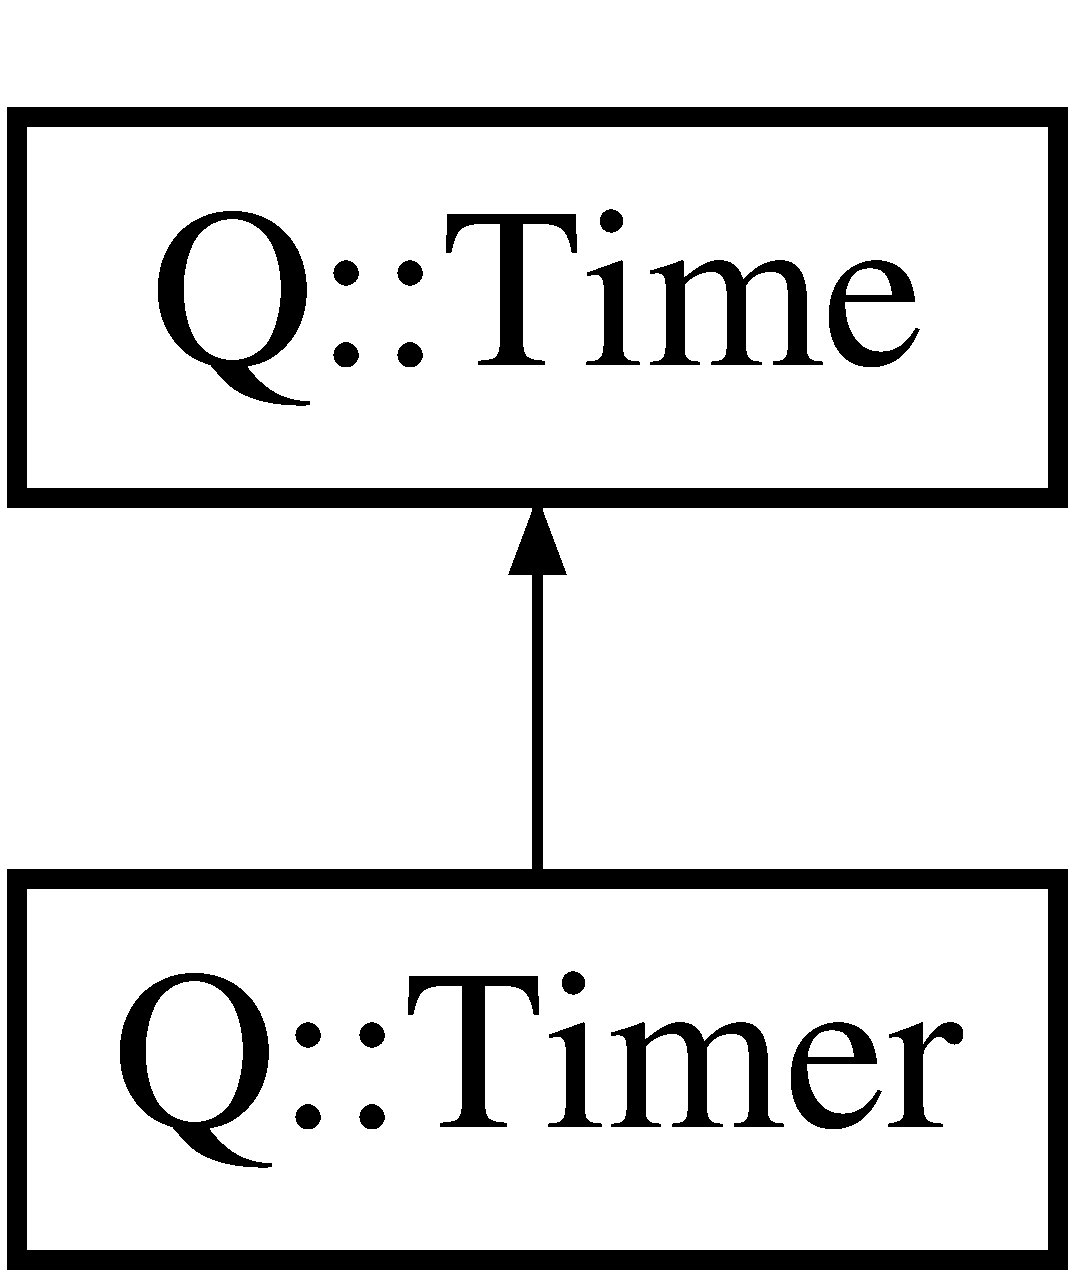
\includegraphics[height=2.000000cm]{class_q_1_1_timer}
\end{center}
\end{figure}
\subsection*{Public Member Functions}
\begin{DoxyCompactItemize}
\item 
\mbox{\Hypertarget{class_q_1_1_timer_acc5dc185878e189ef9de4b032dd4492b}\label{class_q_1_1_timer_acc5dc185878e189ef9de4b032dd4492b}} 
{\bfseries Timer} (unsigned int p\+\_\+\+Hours, unsigned int p\+\_\+\+Minutes, double p\+\_\+\+Seconds)
\item 
\mbox{\Hypertarget{class_q_1_1_timer_a75b48f4b053cac980f84bc6ed431ca40}\label{class_q_1_1_timer_a75b48f4b053cac980f84bc6ed431ca40}} 
void {\bfseries Update} (double p\+\_\+\+Delta\+Time)
\end{DoxyCompactItemize}
\subsection*{Additional Inherited Members}


The documentation for this class was generated from the following files\+:\begin{DoxyCompactItemize}
\item 
D\+:/\+Sam/\+D\+M\+U/\+Year 3/\+I\+M\+A\+T3451 -\/ Final/\+Animation project repo/\+Animation Tool/\+Animation Project/include/Timer.\+h\item 
D\+:/\+Sam/\+D\+M\+U/\+Year 3/\+I\+M\+A\+T3451 -\/ Final/\+Animation project repo/\+Animation Tool/\+Animation Project/include/Timer.\+cpp\end{DoxyCompactItemize}

\hypertarget{class_tool_box}{}\section{Tool\+Box Class Reference}
\label{class_tool_box}\index{Tool\+Box@{Tool\+Box}}


Handles the creation and switching of tools.  




{\ttfamily \#include $<$Tool\+Box.\+h$>$}

Inheritance diagram for Tool\+Box\+:\begin{figure}[H]
\begin{center}
\leavevmode
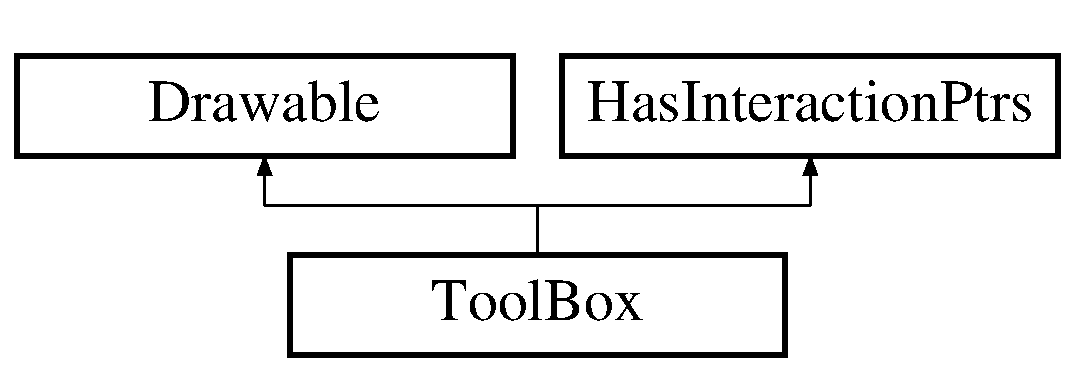
\includegraphics[height=2.000000cm]{class_tool_box}
\end{center}
\end{figure}
\subsection*{Public Member Functions}
\begin{DoxyCompactItemize}
\item 
\mbox{\Hypertarget{class_tool_box_a475f7f91136ff1b2bf6560d59ffe5030}\label{class_tool_box_a475f7f91136ff1b2bf6560d59ffe5030}} 
\hyperlink{class_tool_box_a475f7f91136ff1b2bf6560d59ffe5030}{Tool\+Box} (\hyperlink{struct_interaction_ptrs}{Interaction\+Ptrs} $\ast$p\+\_\+p\+SP)
\begin{DoxyCompactList}\small\item\em Constructor that takes \char`\"{}iteraction\+Ptrs\char`\"{} which contains most of the useful classes that tools need to interact with. \end{DoxyCompactList}\item 
\mbox{\Hypertarget{class_tool_box_ac2512eeee3fb8915bb20eaa07f30bca0}\label{class_tool_box_ac2512eeee3fb8915bb20eaa07f30bca0}} 
void \hyperlink{class_tool_box_ac2512eeee3fb8915bb20eaa07f30bca0}{Update} (float p\+\_\+\+Delta\+Time)
\begin{DoxyCompactList}\small\item\em Update function. \end{DoxyCompactList}\item 
\mbox{\Hypertarget{class_tool_box_ac3414410d0d14deb45099e75b17a9fe4}\label{class_tool_box_ac3414410d0d14deb45099e75b17a9fe4}} 
void \hyperlink{class_tool_box_ac3414410d0d14deb45099e75b17a9fe4}{On\+Mouse\+Click} (sf\+::\+Mouse\+::\+Button p\+\_\+\+Button, bool p\+\_\+\+State)
\begin{DoxyCompactList}\small\item\em On\+Mouse\+Click callback function, registered to the input handlers mouse click signal. \end{DoxyCompactList}\item 
\mbox{\Hypertarget{class_tool_box_a08a321df9ac5a75abbd1a300d28ff117}\label{class_tool_box_a08a321df9ac5a75abbd1a300d28ff117}} 
void \hyperlink{class_tool_box_a08a321df9ac5a75abbd1a300d28ff117}{On\+Mouse\+Move} (sf\+::\+Vector2i p\+\_\+\+Window\+Pos, sf\+::\+Vector2f p\+\_\+\+World\+Pos)
\begin{DoxyCompactList}\small\item\em On\+Mouse\+Move callback function, registered to the input handlers mouse move extra signal. \end{DoxyCompactList}\item 
\mbox{\Hypertarget{class_tool_box_a69078e5a71a14b9103f981762b5d7860}\label{class_tool_box_a69078e5a71a14b9103f981762b5d7860}} 
void \hyperlink{class_tool_box_a69078e5a71a14b9103f981762b5d7860}{Set\+Active} (bool p\+\_\+b\+Active)
\begin{DoxyCompactList}\small\item\em Set the active state of the current tool. \end{DoxyCompactList}\item 
\mbox{\Hypertarget{class_tool_box_a5d8f199ab6a81fd41e6f6052d87b170d}\label{class_tool_box_a5d8f199ab6a81fd41e6f6052d87b170d}} 
void \hyperlink{class_tool_box_a5d8f199ab6a81fd41e6f6052d87b170d}{Select\+Draw} ()
\begin{DoxyCompactList}\small\item\em Set the draw tool as the currently selected tool. \end{DoxyCompactList}\item 
\mbox{\Hypertarget{class_tool_box_a441285f2023171e76dec4241cdd51b0b}\label{class_tool_box_a441285f2023171e76dec4241cdd51b0b}} 
void \hyperlink{class_tool_box_a441285f2023171e76dec4241cdd51b0b}{Select\+Transform} ()
\begin{DoxyCompactList}\small\item\em Set the transform tool as the currently selected tool. \end{DoxyCompactList}\item 
\mbox{\Hypertarget{class_tool_box_a32473bb26bb4c4a7f98866cf8b435c4e}\label{class_tool_box_a32473bb26bb4c4a7f98866cf8b435c4e}} 
void \hyperlink{class_tool_box_a32473bb26bb4c4a7f98866cf8b435c4e}{Select\+Colour} ()
\begin{DoxyCompactList}\small\item\em Set the colour tool as the currently selected tool. \end{DoxyCompactList}\item 
\mbox{\Hypertarget{class_tool_box_a07c9c626ce1c9002084303a5b6cd3e27}\label{class_tool_box_a07c9c626ce1c9002084303a5b6cd3e27}} 
void \hyperlink{class_tool_box_a07c9c626ce1c9002084303a5b6cd3e27}{Select\+Joint} ()
\begin{DoxyCompactList}\small\item\em Set the joint tool as the currently selected tool. \end{DoxyCompactList}\item 
\mbox{\Hypertarget{class_tool_box_a95b5c8ae8056d48eec3ea16bac91af62}\label{class_tool_box_a95b5c8ae8056d48eec3ea16bac91af62}} 
void \hyperlink{class_tool_box_a95b5c8ae8056d48eec3ea16bac91af62}{draw} (sf\+::\+Render\+Target \&target, sf\+::\+Render\+States states) const
\begin{DoxyCompactList}\small\item\em Draw anything that the currently selected tool needs drawing. \end{DoxyCompactList}\end{DoxyCompactItemize}
\subsection*{Additional Inherited Members}


\subsection{Detailed Description}
Handles the creation and switching of tools. 

The documentation for this class was generated from the following file\+:\begin{DoxyCompactItemize}
\item 
D\+:/\+Sam/\+D\+M\+U/\+Year 3/\+I\+M\+A\+T3451 -\/ Final/\+Animation project repo/\+Animation Tool/\+Animation Project/include/Tool\+Box.\+h\end{DoxyCompactItemize}

\hypertarget{class_transform_tool}{}\section{Transform\+Tool Class Reference}
\label{class_transform_tool}\index{Transform\+Tool@{Transform\+Tool}}


Handles the interaction of transforming an object.  




{\ttfamily \#include $<$Transform\+Tool.\+h$>$}

Inheritance diagram for Transform\+Tool\+:\begin{figure}[H]
\begin{center}
\leavevmode
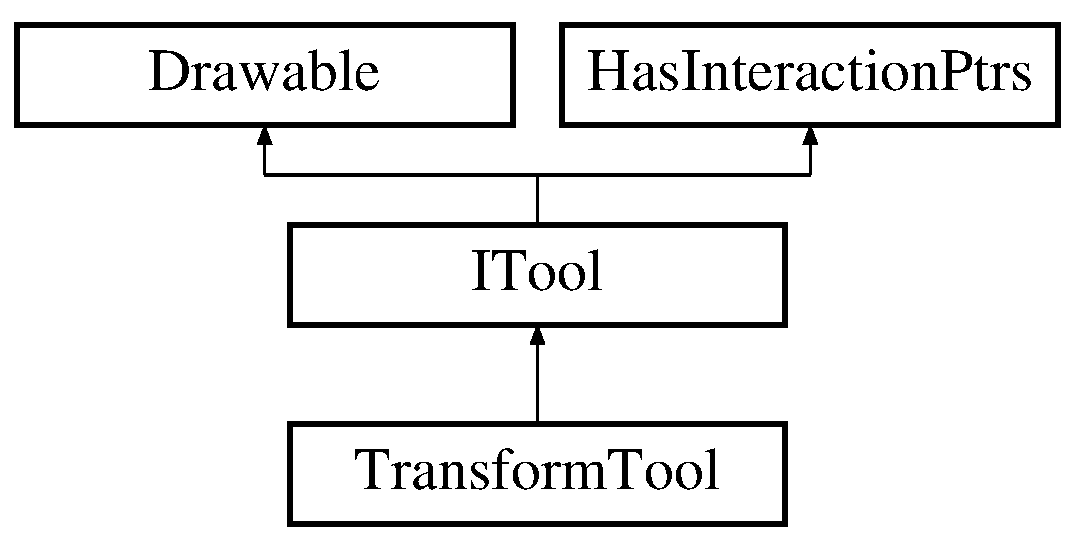
\includegraphics[height=3.000000cm]{class_transform_tool}
\end{center}
\end{figure}
\subsection*{Public Member Functions}
\begin{DoxyCompactItemize}
\item 
\mbox{\Hypertarget{class_transform_tool_a0c5f3caf97efce149d18df2711512358}\label{class_transform_tool_a0c5f3caf97efce149d18df2711512358}} 
\hyperlink{class_transform_tool_a0c5f3caf97efce149d18df2711512358}{Transform\+Tool} (\hyperlink{struct_interaction_ptrs}{Interaction\+Ptrs} $\ast$p\+\_\+p\+SP)
\begin{DoxyCompactList}\small\item\em Constructor that takes the interaction pointer. \end{DoxyCompactList}\item 
\mbox{\Hypertarget{class_transform_tool_aa830f478b61f8de80a6edc8ecb8f2f0d}\label{class_transform_tool_aa830f478b61f8de80a6edc8ecb8f2f0d}} 
void \hyperlink{class_transform_tool_aa830f478b61f8de80a6edc8ecb8f2f0d}{Update} (float p\+\_\+\+Delta\+Time) override
\begin{DoxyCompactList}\small\item\em Update method. \end{DoxyCompactList}\item 
\mbox{\Hypertarget{class_transform_tool_a4716a3bdf7c72190fa7a09f64a94d58f}\label{class_transform_tool_a4716a3bdf7c72190fa7a09f64a94d58f}} 
void \hyperlink{class_transform_tool_a4716a3bdf7c72190fa7a09f64a94d58f}{On\+Mouse\+Click} (sf\+::\+Mouse\+::\+Button p\+\_\+\+Button, bool p\+\_\+b\+State) override
\begin{DoxyCompactList}\small\item\em Callback for mouse click event. \end{DoxyCompactList}\item 
\mbox{\Hypertarget{class_transform_tool_a342c8e953914bf6c97d70eb5aa0accef}\label{class_transform_tool_a342c8e953914bf6c97d70eb5aa0accef}} 
void \hyperlink{class_transform_tool_a342c8e953914bf6c97d70eb5aa0accef}{draw} (sf\+::\+Render\+Target \&target, sf\+::\+Render\+States states) const
\begin{DoxyCompactList}\small\item\em Draw method for drawing all the handles. \end{DoxyCompactList}\end{DoxyCompactItemize}
\subsection*{Additional Inherited Members}


\subsection{Detailed Description}
Handles the interaction of transforming an object. 

The documentation for this class was generated from the following file\+:\begin{DoxyCompactItemize}
\item 
D\+:/\+Sam/\+D\+M\+U/\+Year 3/\+I\+M\+A\+T3451 -\/ Final/\+Animation project repo/\+Animation Tool/\+Animation Project/include/Transform\+Tool.\+h\end{DoxyCompactItemize}

%--- End generated contents ---

% Index
\backmatter
\newpage
\phantomsection
\clearemptydoublepage
\addcontentsline{toc}{chapter}{Index}
\printindex

\end{document}
